\documentclass[12pt,french,twoside]{report}
\usepackage[cyr]{aeguill}
\usepackage[french]{babel}
\usepackage[utf8]{inputenc}
\usepackage{amsthm}
\usepackage{amssymb}
\usepackage{graphicx}
\usepackage{chemist}
\usepackage[french]{algorithm2e}
\usepackage[margin=2.5cm]{geometry}


\setcounter{secnumdepth}{3}



% Title Page
\title{Algorithmique pour les peptides non ribosomiques}
\author{Yoann Dufresne}

\begin{document}
\maketitle
\tableofcontents

\chapter{Les peptides non ribosomiques}

\section{Synthèse non-ribosomique}

\subsection{Introduction}

\paragraph{}Afin de bien comprendre la voie de synthèse non ribosomique, commençons par quelques rappels rapides sur la synthèse des protéines classiques.
Les protéines sont assemblées dans la cellule par un organite appelé ribosome.
Les ARN messagers sont les vecteurs de l'information génétique.
Ils sont la réplication d'un morceau d'ADN qui sera traduit par triplets de nucléotides (appelés codons) en chaîne d'acides aminés.
Les 64 codons possibles ($4^3$ nucléotides) sont traduits en 20 acides aminés appelés acides aminés protéinogènes (justement car ils interviennent dans la synthèse classique de protéines).
Ces acides aminés sont tous composés d'un même squelette atomique autorisant deux liaisons et permettant ainsi la formation de chaînes peptidiques.
Sur le squelette est ancrée une chaîne latérale variant d'un acide aminé à l'autre, leur donnant leur spécificité (voir figure \ref{chaine_pep}).
Les deux liaisons qu'effectuent le squelette sont supportées par un groupement amine ($NH_2$) et un groupement carboxyle ($C(=O)OH$).
Ces deux groupements se lient entre eux en chaîne et créent ainsi la protéine.

\begin{figure}[h!]
  \begin{center}
    \includegraphics[width=350px]{Figures/bio/Intro/chaine_pep.jpg}
    \caption{\label{chaine_pep}Présentation d'une chaîne peptidique.
    Chaque trait pointillé vertical sépare un acide aminé d'un autre et le trait horizontal sépare le squelette de la chaîne latérale des acides aminés.}
  \end{center}
\end{figure}

\paragraph{}Une fois assemblée, une protéine se replie sur elle même et les caractéristiques structurelles et physico-chimiques qui en découlent lui donnent son activité.
Plus précisément, les propriétés des éléments en contact avec l'extérieur de la protéine (les atomes qui ne se retrouvent pas enfermés au milieu du repliement) déterminent l'activité de celle-ci.
Ces propriétés sont donc très dépendantes du repliement et des types des acides aminés exposés.



\subsection{Généralités sur les peptides non ribosomiques}
\paragraph{}Les peptides non ribosomiques (Non Ribosomal Peptide (NRP)) sont des petits polymères synthétisés par certaines bactéries et certains champignons unicellulaires.
Tout comme les protéines classiques, les NRP sont des molécules résultant d'assemblages de briques de base.
Cependant, comme le nom l'indique, la voie de synthèse d'un NRP est différente de celle des protéines.
Cette voie de synthèse comporte une étape supplémentaire (Voir figure \ref{global}).
Comme nous venons de le présenter, lors d'une création classique de protéine, l'ADN est transcrit en ARN qui lui même est traduit en protéine.
Ici, la protéine produite n'est pas le produit final mais une \textit{enzyme modulaire} agissant seule ou en complexe afin d'assembler les NRP.
Ces complexes sont appelés des synthétases (Non Ribosomal Peptide Synthetase (NRPS)).

\begin{figure}[h!]
  \begin{center}
    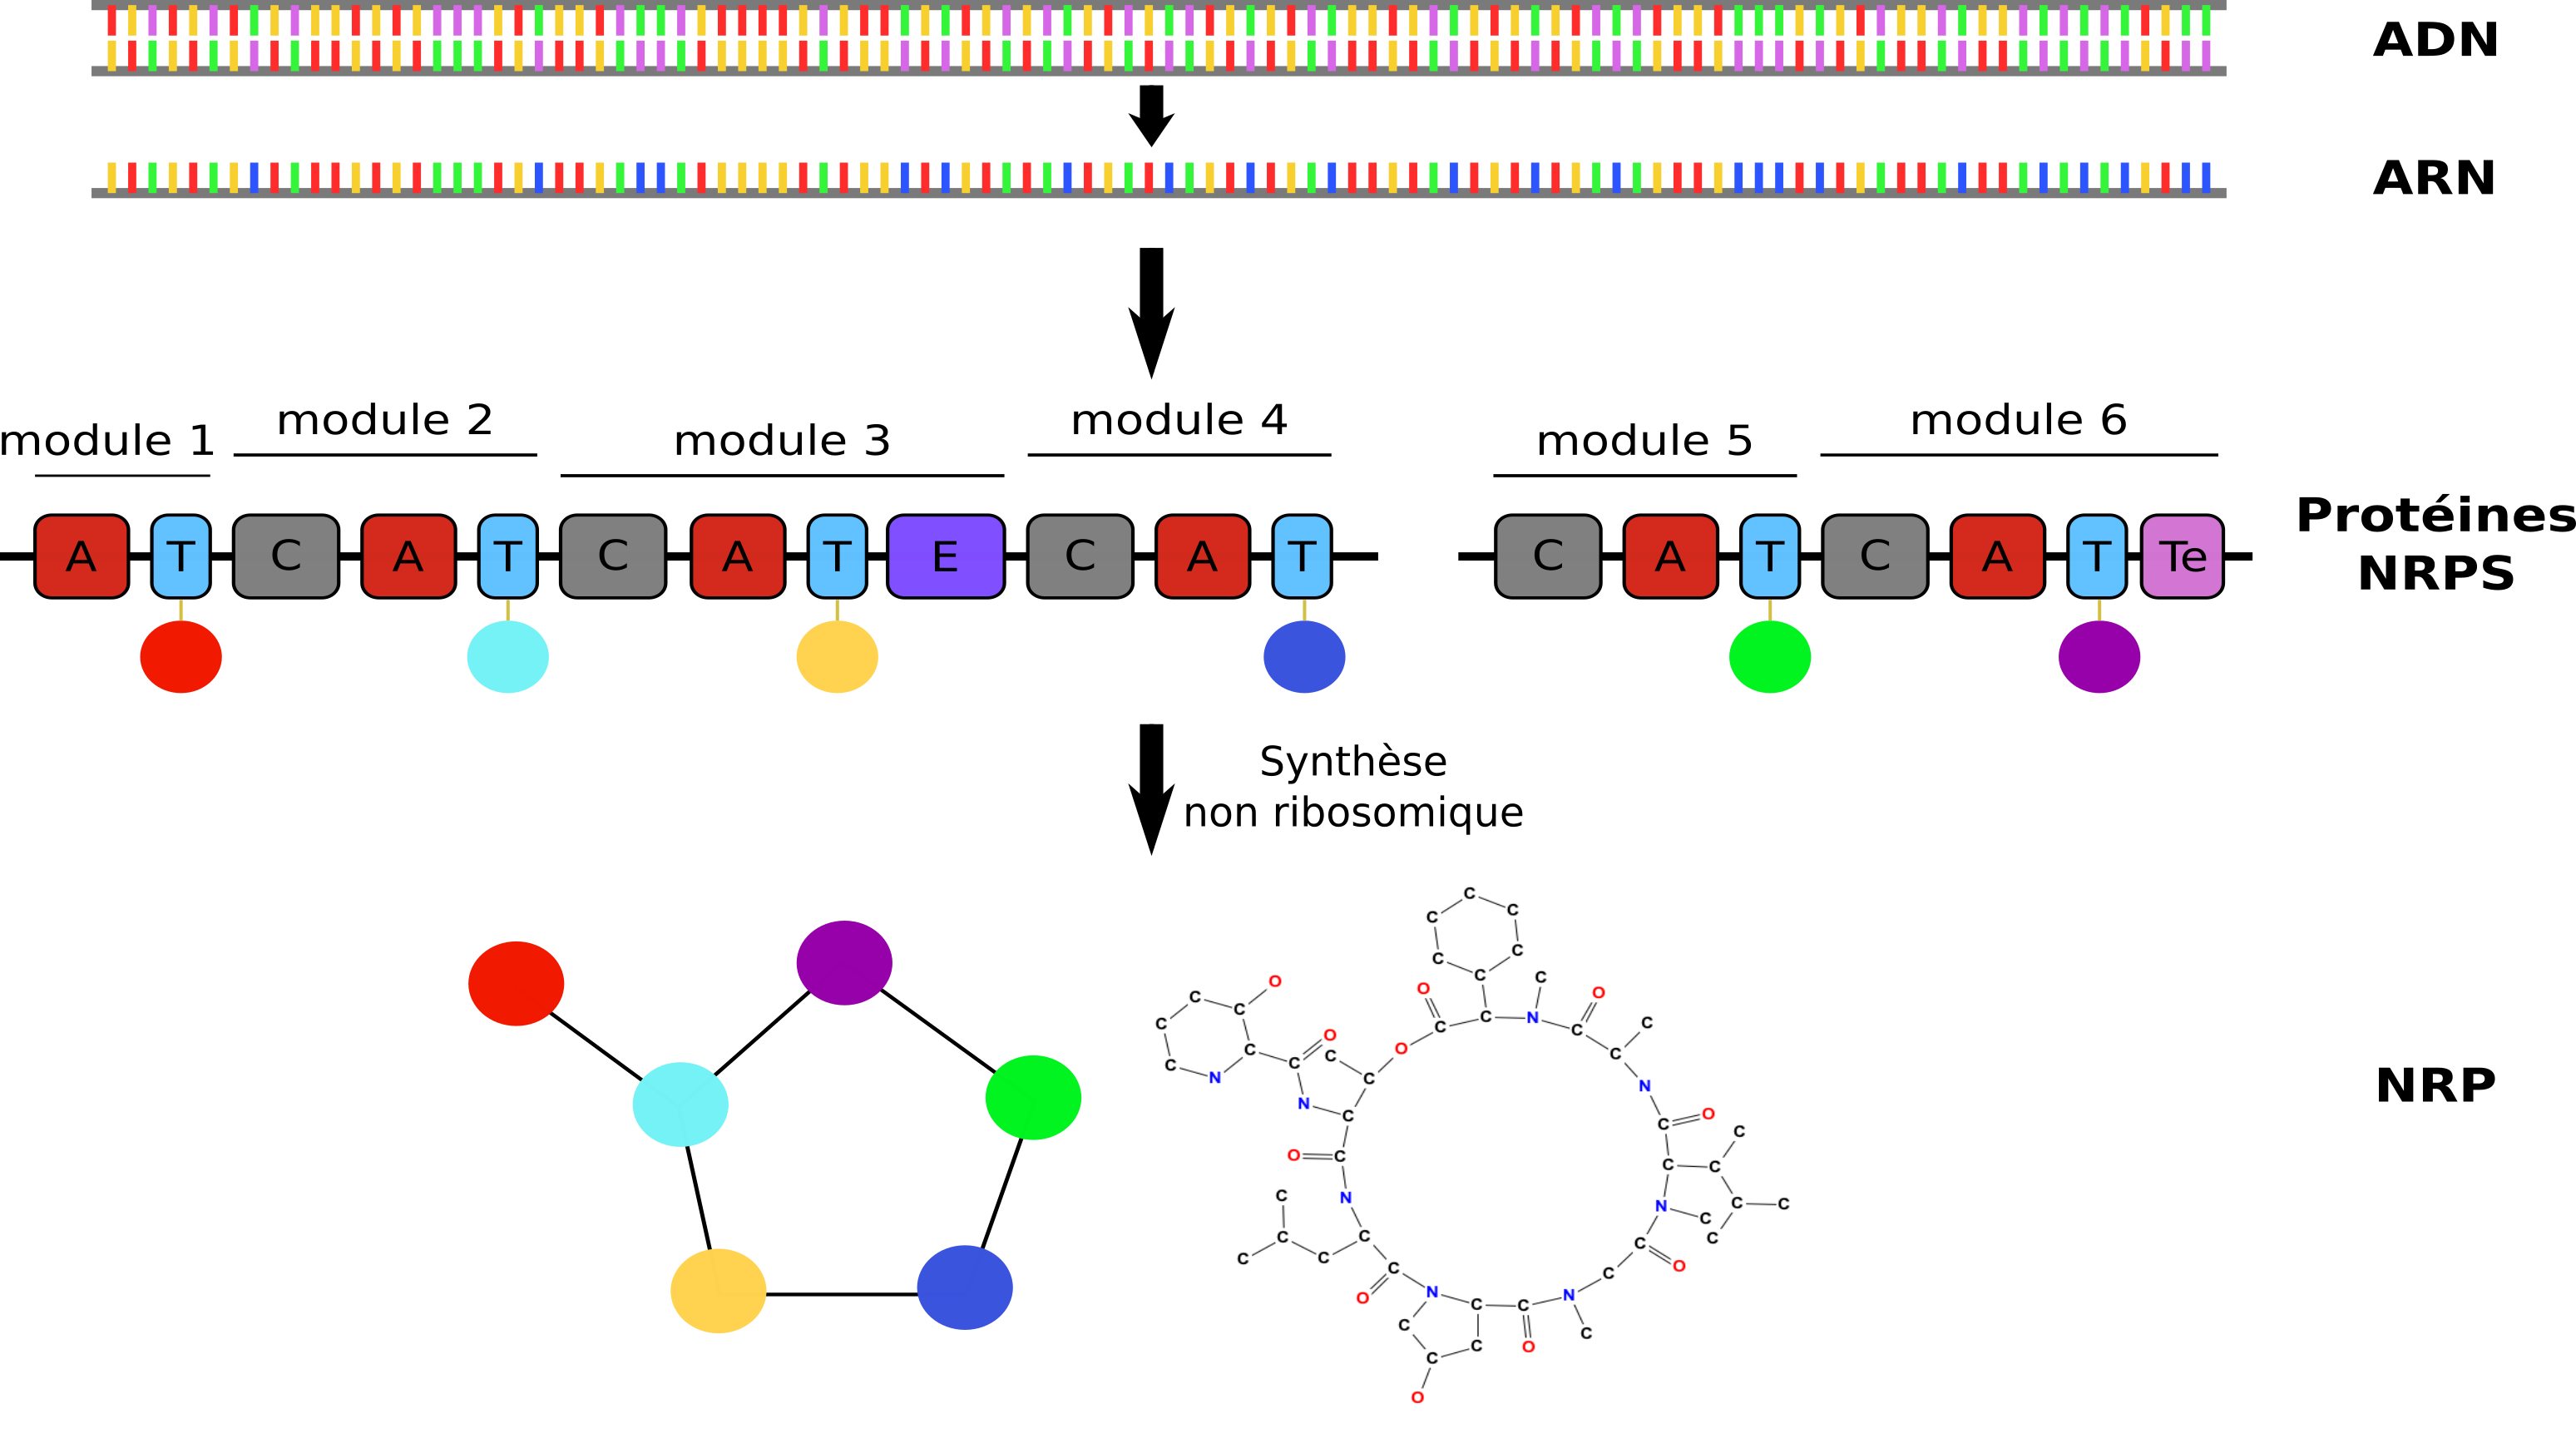
\includegraphics[width=450px]{Figures/bio/Intro/synthese.png}
    \caption{\label{global}Voie de synthèse non ribosomique~:
    Groupés en clusters, les gènes codant la protéine NRPS sont transcrits puis traduits par le ribosome.
    Les modules A de la NRPS capturent ensuite des monomères (billes de couleur ici) dans l'environnement afin des les assembler.
    Enfin, le NRP assemblé est relâché pour aller effectuer sa tâche.
    }
  \end{center}
\end{figure}

\subsubsection{Les monomères}

\begin{figure}[h!]
  \begin{center}
    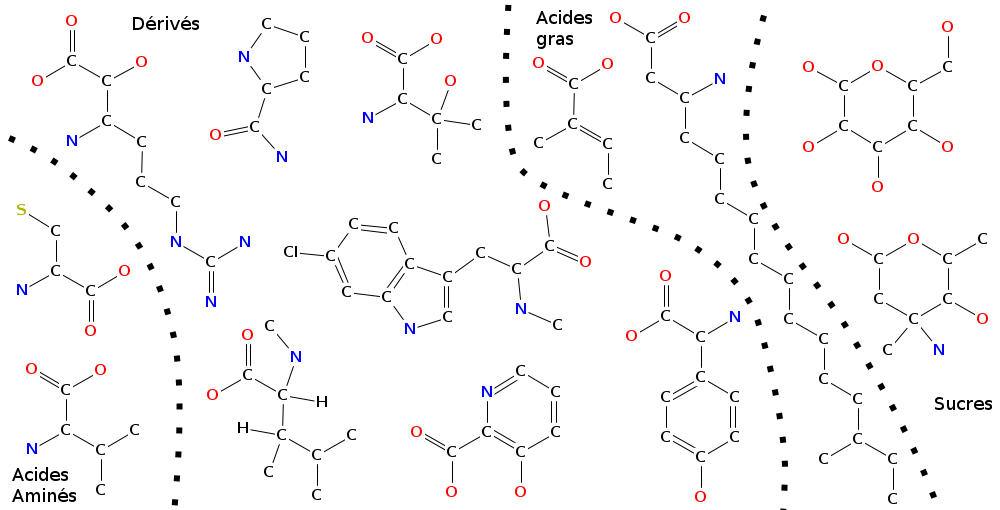
\includegraphics[width=450px]{Figures/bio/Intro/monos/monos.png}
    \caption{\label{monomers_example}Patchwork de monomères NRP.
    En bas à gauche se trouvent des acides aminés classiques.
    Le plus long monomère est un acide gras.
    Entre les deux se trouvent des variants d'acides aminés classiques.
    En haut à droite deux  sucres.}
  \end{center}
\end{figure}

\paragraph{}Là où les protéines classiques sont à majorité composées des 20 acides aminés standards, la synthèse non ribosomique incorpore plusieurs centaines de briques de base différentes.
Ces briques de base sont appelées des {\em monomères}.
La base de données de référence des NRP compte pour le moment 533 monomères différents.
Les monomères peuvent provenir de différents groupes.
Parmi ces monomères, on compte les 20 acides aminés standards ainsi qu'un grand nombre de dérivés proches.
Après plusieurs modifications que nous détaillerons plus tard, il est par exemple possible d'obtenir des monomères méthylés ou oxydés (voir figure \ref{monomers_example}).
On peut également citer les sucres et les acides gras comme faisant partie des monomères candidats à l'inclusion dans des NRP.


\subsubsection{Les structures peptidiques}

\begin{figure}[h!]
  \begin{center}
    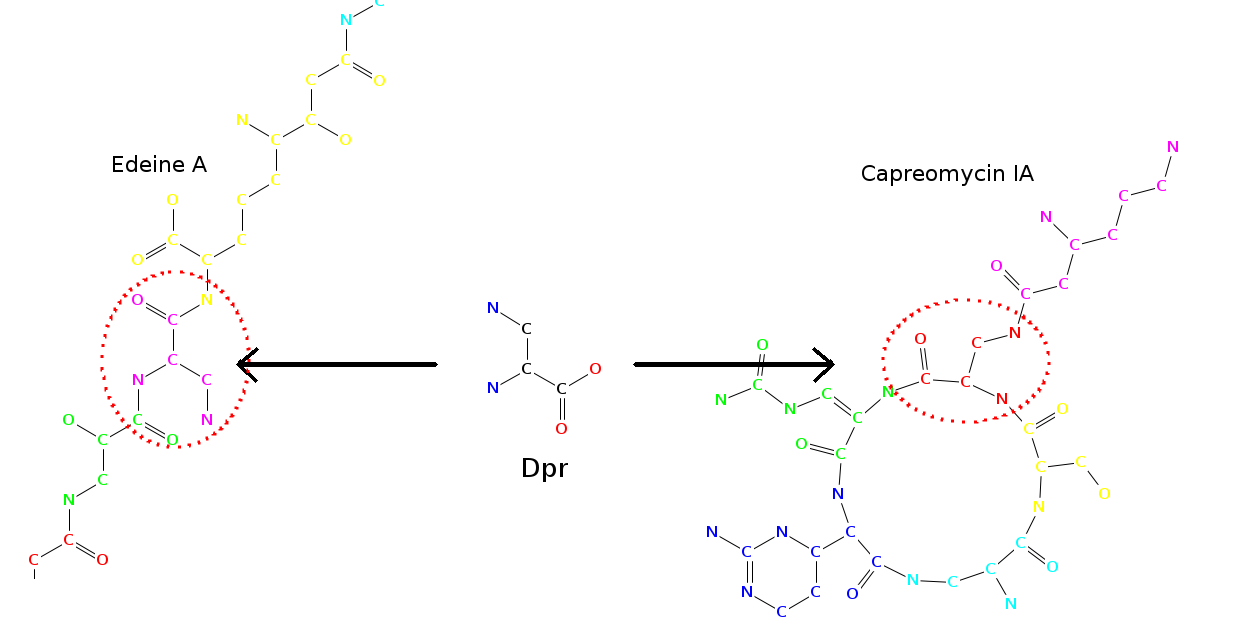
\includegraphics[width=400px]{Figures/bio/Intro/Dpr/2-3_liaisons.png}
    \caption{\label{DPR_incl}Deux exemples d'inclusion du monomère Dp~:
    Au sein de l'Edeine A, seules les deux liaisons classiques du squelette peptidique sont effectuées entre le Dpr (en rose) et les autres monomères.
    Au sein de la Capreomycin IA, une troisième liaison est effectuée par le Dpr (en rouge) depuis son groupement amine ($NH_2$) de la chaîne latérale.}
  \end{center}
\end{figure}

\paragraph{}Les NRPS peuvent arranger les monomères au sein des NRP avec une certaine souplesse.
Certains monomères possèdent plus de deux groupements capables de se lier.
Ainsi sur l'exemple de la figure \ref{DPR_incl}, on peut constater que le monomère nommé Dpr (acide 2,3-diamonopropionique) possède un groupement amine supplémentaire à celui déjà présent dans le squelette des acides aminés classiques.
Ce groupement en bout de chaîne latérale autorise le Dpr à se lier 3 fois et ainsi casser la linéarité de la molécule assemblée.
Ces monomères permettent ainsi d'obtenir des structures à embranchements.


\subsubsection{Les liaisons inter-monomères}

\paragraph{}Classiquement les liaisons au sein de peptides se font par le rapprochement d'un groupe carboxyle d'un monomère vers le groupe amine d'un autre.
Au sein des NRP plusieurs autres types viennent compléter les liaisons possibles et augmentent ainsi la diversité possible des structures.
La liaison peptidique classique reste tout de même la principale liaison effectuée entre monomères.
En dehors de celle-ci, nous pouvons lister trois différents types de liaisons NRP.

\paragraph{}Le premier type de liaison inclut un monomère contenant un atome de soufre.
Comme dans des protéines classiques les monomères soufrés peuvent effectuer des ponts disulfure (liaison entre deux atomes de soufre en perdant deux atomes d'hydrogène).
Cependant ce type de liaison n'est pas le seul impliquant un soufre.
Comme nous le verrons plus tard lors de la description des modules NRPS Cy, l'atome de soufre peut également intervenir dans une cyclisation entre deux monomères en perdant son atome d'hydrogène de la même manière que lorsqu'il réalise un pont disulfure (voir figure \ref{Cy_link}).

\begin{figure}[h!]
  \begin{center}
    \includegraphics[width=400px]{Figures/bio/Intro/reactions/Cy.jpg}
    \caption{\label{Cy_link}Exemple de liaison effectuée par un domaine Cy}
  \end{center}
\end{figure}

\paragraph{}Le second type de liaison implique au moins un monomère contenant un cycle aromatique (cycle imidazole ou benzène).
Dans les deux cas, c'est un atome d'hydrogène qui est arraché au cycle afin de pouvoir y lier un monomère.
Lors d'une liaison d'un cycle imidazole, c'est l'un des deux carbones voisins dans le cycle qui perdra un de ses hydrogènes au profit de la liaison avec l'autre monomère.
Dans le cas d'un benzène (Voir figure \ref{benzene}), c'est la présence d'un oxygène accroché au cycle qui permettra une affinité avec les carbones voisins.

\begin{figure}[h!]
  \begin{center}
    \includegraphics[width=400px]{Figures/bio/Intro/reactions/aro.jpg}
    \caption{\label{benzene}Exemple de liaison effectuée au sein d'un cycle benzène}
  \end{center}
\end{figure}

\paragraph{}Enfin, le dernier type de liaison que nous allons décrire implique au moins un monomère de la catégorie des sucres (Glucose ou Arabinose par exemple).
Les sucres inclus dans les NRP connus sont toujours cyclisés.
Ils se lient par perte d'un groupement OH présent sur un carbone voisin de l'oxygène du cycle.
Face à eux, le monomère complémentaire ne perdra lui qu'un hydrogène pour former ainsi une molécule d'eau expulsée.

\begin{figure}[h!]
  \begin{center}
    \includegraphics[width=400px]{Figures/bio/Intro/reactions/ose.jpg}
    \caption{\label{ose}Exemple de liaison effectuée avec un sucre}
  \end{center}
\end{figure}

\paragraph{}Cette diversité dans la façon de lier les monomères accompagnée du nombre de sites de liaisons candidats explique la diversité structurelle présente au sein des NRP.
Sur la figure \ref{peps_example}, vous pouvez voir cette diversité s'exprimer au travers du grand nombre de structures différentes.

\begin{figure}[h!]
  \begin{center}
    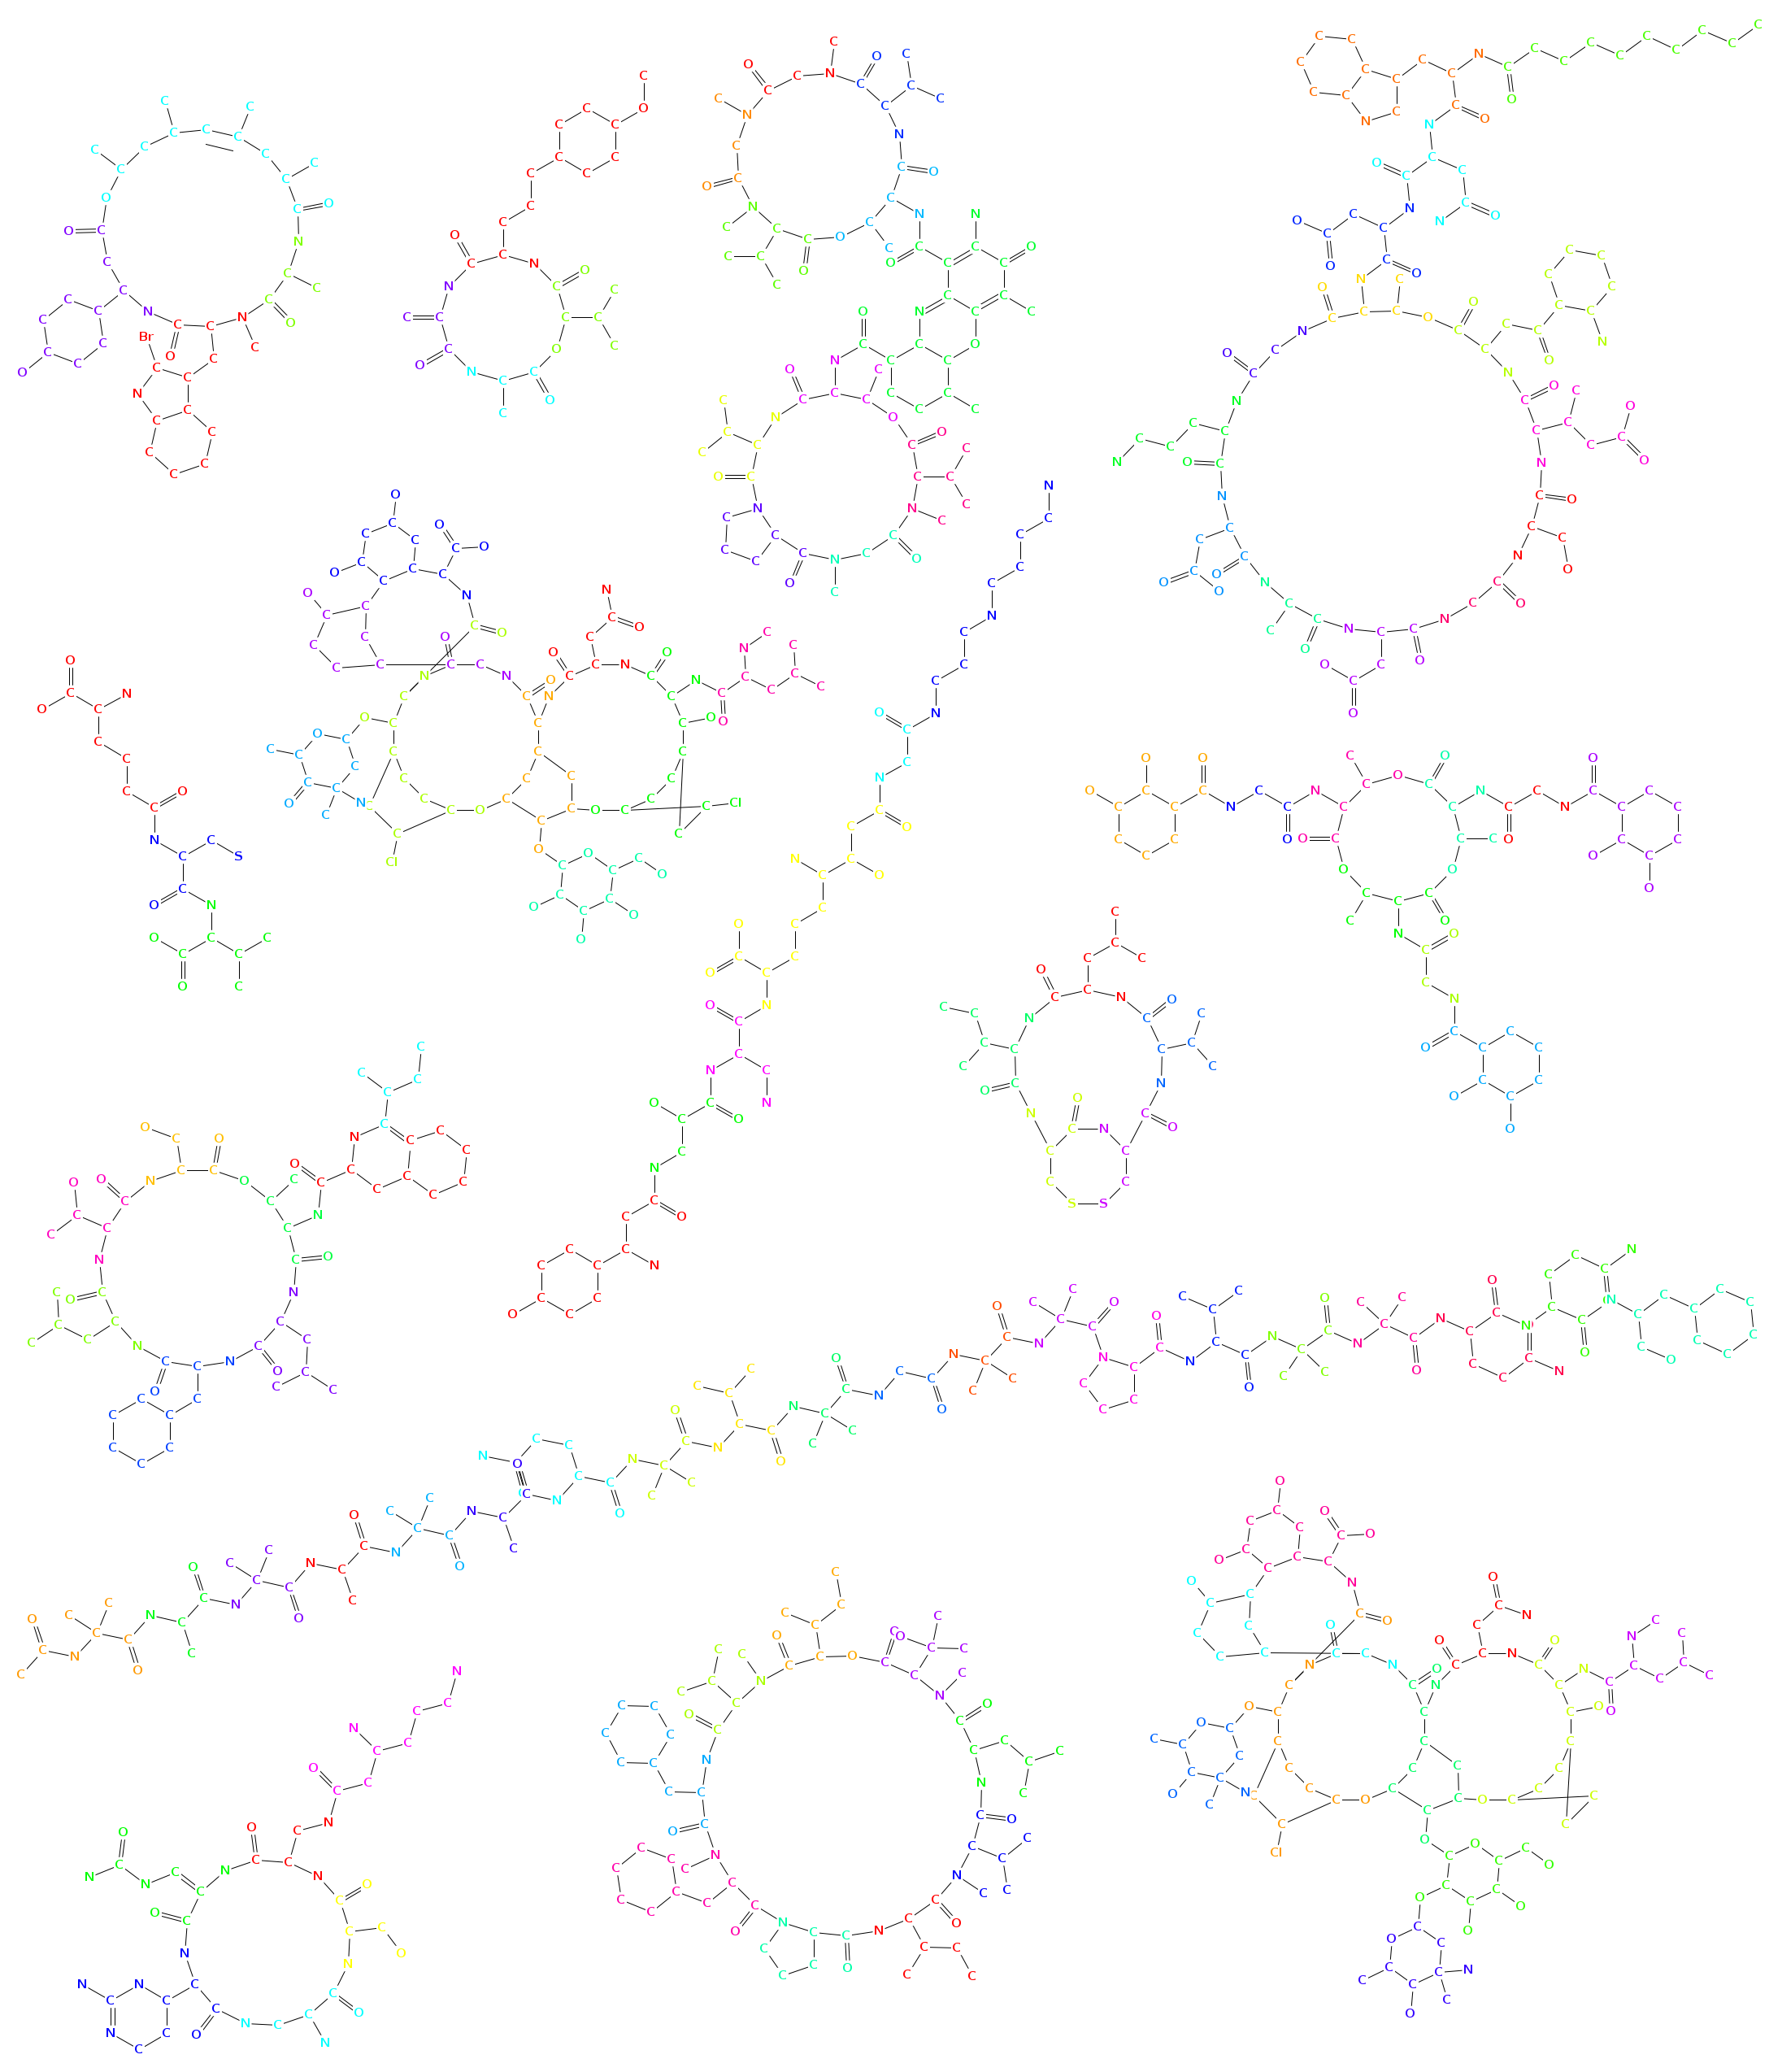
\includegraphics[width=450px]{Figures/bio/Intro/NRPs/peps.png}
    \caption{\label{peps_example}Patchwork de NRP}
  \end{center}
\end{figure}


\subsubsection{Les activités}

\paragraph{}Les NRP présentent une grande diversité d'activités, souvent cruciales pour leurs producteurs.
Beaucoup de NRP recensés sont par exemple des antibiotiques.
Par exemple, la célèbre molécule de pénicilline est synthétisée à partir d'un précurseur NRP appelé ACV~\cite{queener_molecular_1990}.
La diversité d'activités peut être expliquée par les grandes variations de structures et de compositions par rapport aux protéines.
Les différentes structures et divers monomères imposent aux NRP d'opter pour des repliements différents des protéines classiques.
Les contraintes structurelles permettent des repliements difficiles pour des molécules linéaires.
Les activités spécifiques aux NRP sont obtenues grâce à ces repliements.

\paragraph{}Effectuer un assemblage non ribosomique est très consommateur en énergie pour l'organisme producteur.
Les complexes enzymatiques à créer sont énormes et leurs gènes peuvent représenter plusieurs pourcents de l'ADN nucléaire.
De plus, contrairement au ribosome, une NRPS ne peut produire qu'un seul NRP (sauf quelques exceptions qui produisent des variants proches).
Cependant les avantages obtenus grâce aux activités des NRP ont préservé ces gènes au cours du temps.


\subsection{Généralité sur les synthétases}

\paragraph{}Comme nous l'avons vu dans la courte introduction précédente, les synthétases assemblant les NRP sont des protéines issues d'une synthèse classique.
Chaque NRPS est un complexe enzymatique extrêmement grand dont la taille est parfois à comparer à un ribosome (TODO : exemple taille en aa).
Cependant, contrairement à un ribosome, les NRPS sont spécialisés.
Une NRPS ne peut produire qu'un seul type de NRP.
Elles sont organisées en modules consécutifs qui capturent modifient et intègrent un monomère au NRP\cite{schwarzer_nonribosomal_2003,marahiel_modular_1997}.
Chacun de ces modules peut à son tour être découpé en domaines fonctionnels.
Généralement un module est constitué de 3 domaines principaux et éventuellement de domaines optionnels\cite{finking_biosynthesis_2004}.
Un module standard est d'abord composé d'un domaine de condensation (C) effectuant la liaison du peptide déjà formé au monomère en cours d'inclusion puis d'un module d'adénilation (A) permettant la capture du monomère à insérer et d'un module de thiolation (T) effectuant la fixation du monomère capturé et le transfert du NRP depuis le domaine C précédent au domaine C suivant.
Il se peut qu'un ou plusieurs domaines modifiant le monomère inclus, soient présents entre le domaine A et le domaine T.
Le premier module est également une exception à la règle du C-A-T car il ne possède normalement pas de domaine C (Car il n'y a rien à lier).

\begin{figure}[h!]
  \begin{center}
    \includegraphics[width=480px]{Figures/bio/Intro/hc-toxin.png}
    \caption{\label{mibig_hc}Modules NRPS pour la création du peptide HC-Toxin.
    Image issue du site web MiBIG.}
  \end{center}
\end{figure}

\paragraph{}Prenons pour exemple le NRP appelé hc-toxin~\cite{_mibig:_????}.
Le hc-toxin est un peptide non ribosomique composé de 4 monomères.
D'après la base de données MiBig couplée à celle du NCBI, la synthétase permettant sa création est composée de 5218 acides aminés.
Cette enzyme peut être séparée en 4 modules, incluant chacun un monomère.
Chacun des modules est également découpé en domaines.
Le découpage pour ce NRP est représenté sur la figure~\ref{mibig_hc}.
Aux 4 modules correspondent 4 domaines A, 4 domaines T et 3 domaines C.
On peut également voir un domaine d'épimérisation (modification de l'acide aminé inclus) présent en fin de premier domaine ainsi qu'un domaine C supplémentaire en fin d'enzyme effectuant la cyclisation du peptide.

\subsection{Les domaines principaux}

\subsubsection{Le domaine d'Adénilation (domaine A)}

\paragraph{}Ce domaine porte la spécificité du module dans lequel il se trouve.
Un domaine A donné ne peut capturer qu'un seul type de monomère (sauf quelques exceptions qui peuvent capturer des variants proches).
La séquence d'acides aminés de ce type de domaine varie fortement d'un domaine à l'autre.
Un grand nombre de domaines A différents (plusieurs centaines) sont obtenus grâce à ces variations.
De fait, plusieurs centaines de monomères sont inclus par ces domaines.
Une fois le repliement de la synthétase effectué, les domaines A possèdent une cavité interne effectuant la reconnaissance et l'accueil d'une molécule.
Les acides aminés de la synthétase en contact avec cette cavité vont ``choisir'' le monomère à capturer dans l'environnement.
La taille de la cavité ainsi que les propriétés physico-chimiques de ces acides aminés en contact permettent une affinité forte avec un unique monomère.
Il arrive parfois que le domaine ne soit pas spécifique à un seul monomère mais plutôt à un petit nombre de monomères très proches les uns des autres.
Cependant, ce cas reste rare et, dans la majorité des cas, une NRPS ne crée qu'un seul NRP.

\paragraph{}En 1999, Stachelhaus et al. publient un article analysant la structure de nombreux domaines A~\cite{stachelhaus_specificity-conferring_1999}.
Ils alignent un grand nombre de domaines A pour en extraire les parties conservées et les parties spécifiques au monomère à capturer.
Il apparait que très peu d'acides aminés sont conservés entre domaines A.
Ces quelques acides aminés peuvent cependant servir de marqueurs.
Ces points conservés (et donc a priori très importants), servent de repères vers des acides aminés proches faisant partie de la poche d'accueil du monomère.
Les auteurs extraient un codage déterminant le monomère inclus à partir de 10 acides aminés présents dans la séquence d'un domaine A.
Depuis cet article, ce codage de référence est appelé code de Stachelhaus.


\subsubsection{Le domaine de Thiolation (domaine T)}
%citations : 
%• Biochemical characterization of peptidyl carrier protein (PCP), the thiolation domain of multifunctional peptide synthetases.
%• Portability of the thiolation domain in recombinant pyoverdine non-ribosomal peptide synthetases

\paragraph{}Le but du domaine T est d'assurer la logistique au sein du module dans lequel il est contenu~\cite{stachelhaus_biochemical_1996,calcott_portability_2015}.
Ce domaine est également souvent appelé ``Peptidyl Carrier domain''.
Il est en charge de la récupération et du transfert du peptide en cours de formation.
Chaque domaine T possède un groupement \textit{4’-phosphopantetheine} incluant un ``bras flexible'' qui agrippe et déplace les monomères.
Dans un premier temps, ce bras se plie vers le domaine A voisin pour le lier de manière covalente au monomère.
Dans un second temps, le monomère est mené au site de condensation afin d'être inséré en bout du NRP.
Enfin, le bras se plie dans la direction du domaine de condensation suivant afin de lier le NRP au monomère suivant.
Durant cette étape, le peptide est libéré du domaine T courant pour être laissé à la charge du domaine T suivant.

\begin{figure}[h!]
  \begin{center}
    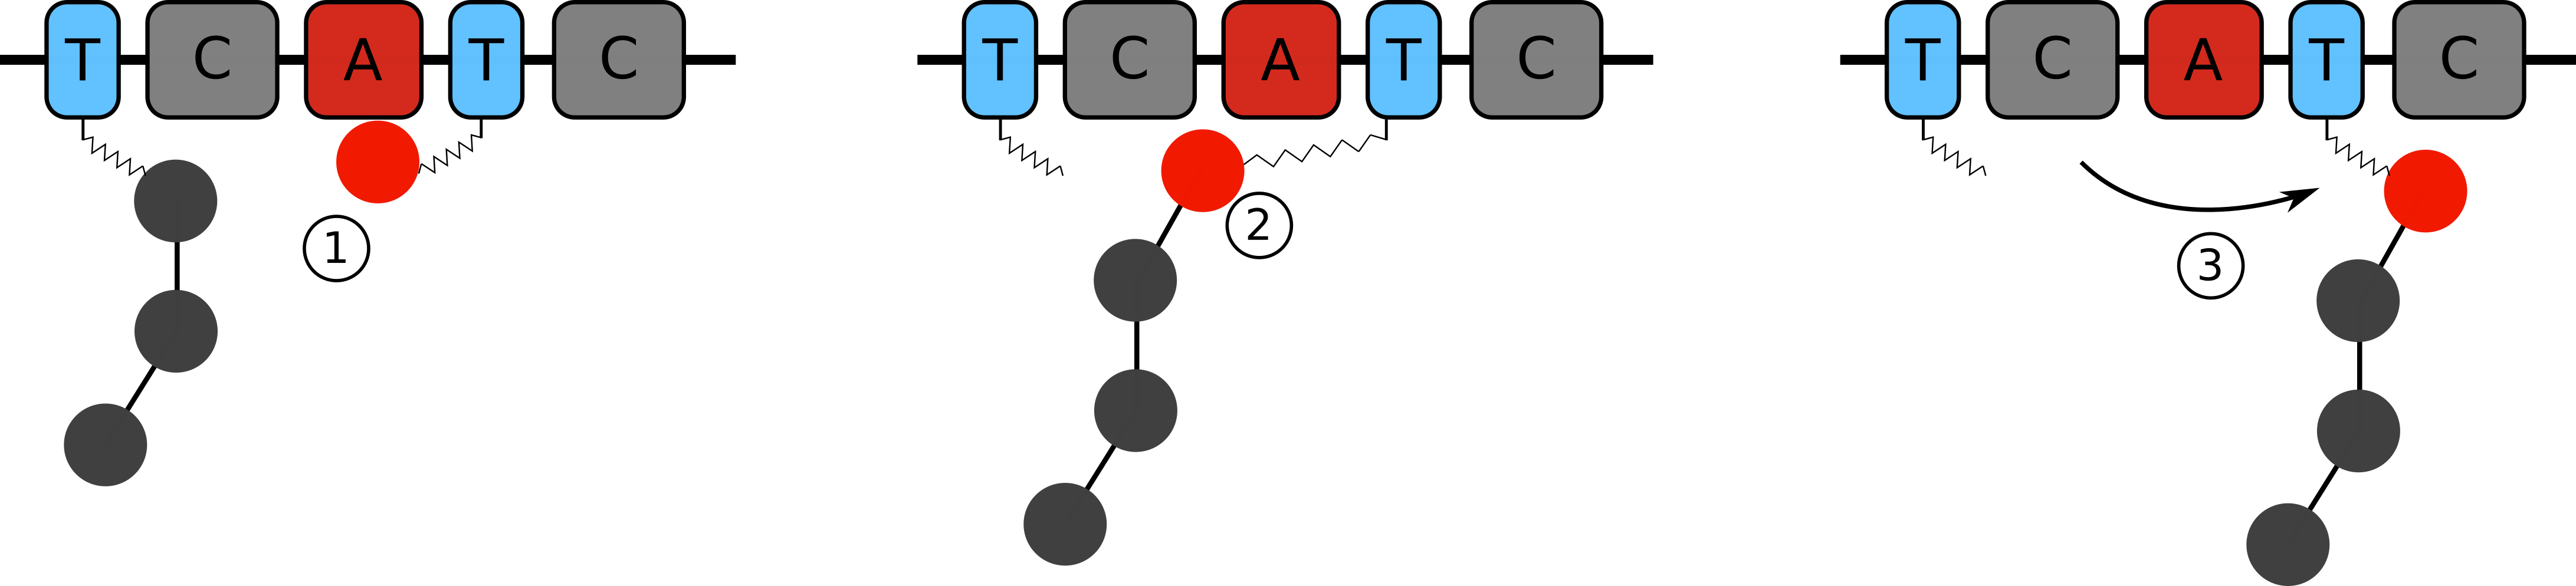
\includegraphics[width=450px]{Figures/bio/Intro/T-domain.png}
    \caption{\label{T_domain}Rôle du domaine T au sein d'une NRPS.
    1~- Liaison entre le monomère capturé par le domaine A et le bras du module T.
    2~- Liaison entre le monomère et le bout de la chaîne peptidique déjà formée.
    3~- Déplacement du peptide vers le domaine C suivant}
  \end{center}
\end{figure}

\subsubsection{Le domaine de Condensation (domaine C)}
%citations :
%• Peptide Bond Formation in Nonribosomal Peptide Biosynthesis, CATALYTIC ROLE OF THE CONDENSATION DOMAIN
%• http://bmcevolbiol.biomedcentral.com/articles/10.1186/1471-2148-7-78

\paragraph{}Le domaine C est par convention considéré comme le premier domaine de chaque module~\cite{stachelhaus_peptide_1998}.
C'est un domaine qui lie le morceau de peptide assemblé par les modules précédents avec le monomère capturé par le domaine A du module courant.
Bien que sa fonction principale reste toujours la même, il existe plusieurs variants~\cite{rausch_phylogenetic_2007} de ce domaine que nous allons décrire par la suite.

\paragraph{Les domaines LCL et DCL}
Les acides aminés capturés par les domaines A existent dans deux configurations différentes dites configurations L (Leavus) et D (Dexter).
Il existe deux domaines C différents pour lier ces molécules.
Le plus standard, lie deux monomères de type L. Le domaine est alors appelé domaine LCL.
Le second lui, lie un monomère D à un L, il est alors appelé domaine DCL.
Ces domaines sont juste deux spécialisations du modèle décrit ci-dessus.

\paragraph{Les domaines C starter (Cs) et C terminal (Ct)}
Comme leurs noms l'indiquent, ces domaines sont en bout de protéines.
Ils ne sont donc pas entourés de deux modules différents mais sont inclus respectivement dans le premier et dernier modules.
Il ne peuvent donc faire la liaison entre deux monomères fixés sur deux bras de domaines T.

\paragraph{}Le domaine Cs capture et lie directement un monomère de l'environnement afin de débuter le peptide.
Cela permet d'inclure par exemple les acides gras car ils ne sont pas reconnus par les domaines A.
Ces modules capturent toujours le même type de monomères mais on ne sait actuellement pas exactement comment cette spécificité est encodée dans l'enzyme.

\paragraph{}Le rôle du domaine Ct est lui un peu plus flou.
Dans certains peptides, ce domaine effectue une liaison entre le dernier monomère et un monomère déjà inclus, créant ainsi un cycle\cite{gao_cyclization_2012}.
Dans d'autres, il lie le dernier monomère avec un monomère spécifique de l'environnement (même procédé que pour le module Cs).
Comme pour le Cs, la spécificité n'est pas encore expliquée.
Il est également possible que les deux comportements soient en fait issus de deux sous-catégories de Ct mais aucune littérature sur le sujet n'a encore été publiée.

\paragraph{Le domaine Cy}
Cette dernière variation du module C standard lie deux monomères voisins en effectuant deux liaisons qui forment un cycle local (voir figure \ref{domaine_Cy}.
Cette liaison est toujours effectuée entre un monomère possédant un atome de soufre près d'un groupement amine (la Cystéine et certaines de ses dérivées) et un monomère avec un groupement hydroxyl.

\begin{figure}[h!]
  \begin{center}
    \includegraphics[width=300px]{Figures/bio/Intro/domainCy_bacitracine.png}
    \caption{\label{domaine_Cy}Cyclisation entre deux monomères par un domaine Cy}
  \end{center}
\end{figure}


\subsubsection{Le domaine de Thioestérase}

\paragraph{}Le domaine Te fait partie du module de terminaison.
Il est le dernier domaine de ce module et vient succéder le domaine T ou les domaines optionnels présents après le T.
C'est un domaine de terminaison qui permet le décrochage et parfois la cyclisation du peptide complètement formé~\cite{trauger_peptide_2000,kohli_thioesterase_2002}.
Ce domaine de séparation n'est pas toujours présent et sa fonction est parfois exprimée par d'autres domaines comme le Ct.


\subsection{Les domaines de transformation monomérique}

\paragraph{}Nous allons à présent parler de quelques domaines optionnels modifiant un monomère capturé par un domaine A.
Ces transformations permettent aux organismes d'obtenir des configurations monomériques peu fréquentes dans leur environnement.


\paragraph{La fonction d'épimérisation (domaines E et C/E)}

Lors de la description des domaines LCL et DCL, nous avons rapidement évoqué la possibilité pour une molécule d'être dans deux conformations différentes tout en possédant pour autant la même composition et structure atomique.
Ces deux conformations sont symétriques l'une de l'autre.
Elles sont appelées Leavus (L) et Dexter (D).

\begin{figure}[h!]
  \begin{center}
    \includegraphics[width=400px]{Figures/bio/Intro/domaineE-bacitracine.png}
    \caption{\label{domaine_E}Épimérisation d'un monomère par un domaine E}
  \end{center}
\end{figure}

\paragraph{}Alors que la majorité de la vie est ``gauchère'' (ne contient que des acides aminés L), les NRPS autorisent l'inclusion de monomères de forme D par la capture d'un monomère L puis sa transformation en conformation D.
Les domaines responsables de ces transformations sont appelés domaines d'\textit{épimérisation}~\cite{calcott_portability_2015}.
Une fois le monomère L lié au reste du peptide par le domaine C, il est emmené auprès du domaine E afin de changer son orientation.
Le fait que cette transformation soit postérieure à la fixation sur le reste du peptide explique l'absence de domaines DCD (Les monomères de droite seront toujours présentés au domaine C avant transformation).
Il arrive parfois que cette transformation du monomère ne soit pas portée par un domaine E mais directement incluse dans le domaine C précédent.
Ce domaine est alors appelé domaine C/E et assure les deux fonctionnalités~\cite{yin_enduracidin_2006,balibar_generation_2005}.


\paragraph{domaine de N-méthylation (NM)}

De la même manière que le domaine E, le domaine NM agit à la suite de la liaison du monomère actuel au morceau de peptide précédemment assemblé.
Ce domaine ajoute un méthyle ($CH_{3}$) sur le groupement amine du monomère courant.

\begin{figure}[h!]
  \begin{center}
    \includegraphics[width=300px]{Figures/bio/Intro/domaineNMe-cyclosporine.png}
    \caption{\label{domaine_NMe}Méthylation d'un monomère par un domaine NM}
  \end{center}
\end{figure}

\paragraph{domaine de formylation}
% http://archiv.ub.uni-marburg.de/diss/z2008/0068/pdf/dgs.pdf

Ce domaine n'existe a priori que pour les modules d'initiation.
Il permet la formylation (ajout d'un groupe C(=O)H) sur le groupement amine du premier monomère~\cite{schonafinger_amide_2007}.

\begin{figure}[h!]
  \begin{center}
    \includegraphics[width=300px]{Figures/bio/Intro/domaineF-gramicidine.png}
    \caption{\label{domaine_F}Formylation d'un monomère par un domaine F}
  \end{center}
\end{figure}


\subsection{Incorporations extra-NRPS}

\paragraph{}Depuis le début de cette partie, nous parlons de synthèse non ribosomique.
Cependant, il arrive que le produit délivré par la synthétase et le produit final trouvé dans l'environnement de la cellule ne soient pas les mêmes.
Lorsque cette différence est constatée, c'est que le peptide a subi une transformation entre la fin de sa synthèse non ribosomique et le moment où il est effectivement en activité.
Toutes les modifications ponctuelles sont effectuées par des enzymes de décoration.
Parfois, il arrive que ce soit une partie complète de la molécule qui ne soit pas NRP.
Il existe des molécules très proches des NRP appelés polyketides qui peuvent venir s'hybrider avec des NRP.
Dans cette partie, nous allons aborder ces deux types de modification/ajout d'un NRP.


\subsubsection{Les enzymes de décoration}

\label{sucres}

\paragraph{}Les clusters de gènes de NRPS ne sont pas uniquement constitués des gènes d'enzymes NRPS.
De nombreux gènes accompagnateurs sont présents, généralement inclus dans le cluster.
Parmi ceux-ci, certains gènes servent à modifier les NRP déjà relâchés par la NRPS.
La \textit{vancomycine} est un très bon exemple de peptide subissant des modifications enzymatiques post-synthèse.

\begin{figure}[h!]
  \begin{center}
    \includegraphics[width=300px]{Figures/bio/Intro/vanco.png}
    \caption{\label{vanco}Modifications post-synthèse NRP pour la vancomycine}
  \end{center}
\end{figure}

\paragraph{}Sur la figure \ref{vanco}, les deux structures entourées en vert se démarquent par rapport au reste de la molécule.
Ce sont deux sucres qui ont été ajoutés après la synthèse (une \textit{vancosamine} et un \textit{D-glucose}).
Les sucres sont des monomères qui ne peuvent pas être capturés par des domaines A.
Ce sont des gènes extérieurs à la NRPS mais faisant partie du cluster, qui sont dédiés à leur capture, transformation et liaison avec la NRP.
Ce phénomène d'ajout de sucre est appelé \textit{glycosylation}.
Comme le suggère \cite{van_wageningen_sequencing_1998}, trois enzymes entrent en action pour incorporer la vancosamine.
La vancosamine n'étant pas naturellement présente dans l'environnement de l'organisme producteur, l'une des enzymes est dédiée à la création de ce sucre à partir du \textit{NDP-4-keto-6-deoxyglucose}.

\paragraph{}La vancomycine possède également deux atomes de Chlore.
Ces deux atomes sont inhabituels pour des NRP et ne sont pas initialement présents au sein de leurs monomères de rattachement.
Il n'existe pas non plus de domaine NRPS capable d'inclure ces atomes.
Van Wageningen dans l'article précédemment cité, montre également que deux enzymes issues du cluster de gènes de la NRPS sont responsables de ces incorporations.
Ce type d'enzyme est appelé enzyme d'halogénation car il est capable d'inclure un atome halogène (Fluor, Clore, Brome, Iode, Astate)

\paragraph{}Pour résumer, les enzymes de décoration post-synthèse sont capables d'effectuer 3 tâches que nous avons découvertes sur l'exemple de la vancomycine :
\begin{itemize}
  \item La synthèse de monomères en modifiant des composants de l'environnement (par exemple, création de vancosamine)
  \item La création de liaisons entre monomères de l'environnement et NRP (par exemple, les sucres de la vancomycine)
  \item La modification de morceaux de monomères déjà inclus dans le NRP (halogénation par exemple)
\end{itemize}

Toutes ces enzymes augmentent à nouveau la combinatoire des molécules potentiellement créées.



\subsubsection{Les PKS}

\paragraph{}Les PKS (Polyketyde Synthase)~\cite{shen_polyketide_2003,staunton_polyketide_2001} sont, tout comme les NRPS, des enzymes modulaires synthétisant des polymères complexes par assemblage de monomères.
Cependant, contrairement aux NRPS, les PKS n'incorporent pas de monomères directement formés mais construisent les PK (Polyketyde) par ajouts successifs de monomères ne faisant que quelques atomes (moins de 10 en général).
De la même manière que les domaines A des NRPS capturent des monomères spécifiques, certains domaines PKS sont spécialisés pour effectuer des réactions d'ajout de quelques atomes au PK en création.
Tout comme les NRP, les PK sont des molécules très coûteuses en énergie pour la production mais très utiles pour les organismes qui les synthétisent.
Sur la figure \ref{pks} nous montrons le processus de synthèse d'une PK.

\begin{figure}
  \begin{center}
    \includegraphics[width=400px]{Figures/bio/Intro/PKS.png}
    \caption{\label{pks}Synthèse d'une epsilon-rhodomycinone
    Comme pour les NRPS, les PKS sont constitués de modules fonctionnels.
    Sur cet exemple, on peut voir que certains modules sont utilisés itérativement.
    La longue chaîne carbonée de la première étape est créée par une utilisation de 9 fois le même module.
    Tout comme les NRP, les PK peuvent être modifiés après libération par le PKS (étapes 5 à 10 ici).
    Source de l'image : en.wikipedia.org/wiki/Polyketide\_synthase}
  \end{center}
\end{figure}

\paragraph{}Plusieurs NRP sont hybrides avec des PK, le cluster de gènes est alors composé de gènes NRPS et PKS.
Il existe alors deux moyens de créer ces hybrides.
Soit la PK est créé séparément du NRP et les deux sont liés post-synthèse par des enzymes similaires aux enzymes décoratrices décrites précédemment.
Soit la PKS et la NRPS sont produits simultanément et s'assemblent pour former un gros complexe enzymatique hybride.
Le NRP-PK est alors directement formé pendant la synthèse en faisant passer le polymère en formation de module en module (qu'ils soient NRPS ou PKS).
A nouveau, cette hybridation avec d'autres types de polymères augmente la quantité de molécules différentes possibles.









\section{Les outils bioinformatiques pour l'annotation et l'analyse des NRP/NRPS}

\paragraph{}Après avoir présenté les NRP ainsi que leurs voies de synthèse, nous allons nous attarder sur les outils bio-informatiques qui s'y intéressent.
Les outils que nous allons présenter ici se focalisent soit sur les NRPS soit sur les NRP, c'est pourquoi la présentation séparera distinctement ces deux types d'outils.
Pour chacune de ces catégories, nous allons également distinguer deux sous-catégories.
La première portera sur les outils effectuant l'annotation des données.
Pour les NRPS, l'annotation correspondra à la phase de recherche de gènes NRPS dans le génome ainsi qu'à l'identification des différentes briques contenues dans ces gènes (entre autre les modules).
Pour les NRP, l'annotation correspondra à la phase d'identification et de décomposition des structures monomériques présentes dans des molécules.
La seconde sous-catégorie présentera les moyens d'archivage et de mise à disposition des informations récoltées par les outils d'annotation.
Cette partie rassemblera les différentes bases de données, dédiées ou non, et contenant une ou plusieurs informations à propos des NRPS ou NRP.

\subsection{Les outils d'annotation de NRPS}

\paragraph{}Dans cette partie, nous allons présenter les outils bioinformatiques permettant la découverte et l'annotation de NRPS depuis le génome.
Cette recherche pourra être effectuée par étapes successives en commençant par la détection des clusters de gènes, en poursuivant par l'annotation des domaines des NRP et en finissant par les détections spécifiques aux domaines détectés.

\subsubsection{Détection de clusters de gènes}

\paragraph{}L'information des clusters de gènes est très importante pour comprendre les formes finales de NRP.
La détection des clusters nous permet d'identifier l'ensemble des gènes impliqués dans la synthèse d'un NRP et pas uniquement ceux codant une NRPS.
Avoir accès à l'ensemble des gènes d'un cluster nous autorise par exemple la détection des transformations post-synthèse qui peuvent modifier un NRP.

\paragraph{}Il existe de nombreuses techniques de recherche de clusters de gènes.
Certains outils génériques comme CLUSEAN\cite{weber_clusean:_2009} détectent tout type de clusters.
Il existe également des techniques spécialisées pour détecter directement des clusters de gènes de métabolites secondaires.
Par exemple, le logiciel CASSIS~\cite{wolf_cassis_2016} exploite des propriétés de régions promotrices pour découvrir et classifier ces clusters.

\paragraph{}De nombreux autres logiciels encore plus spécialisés existent.
Il est aussi possible de découvrir des clusters de métabolites secondaires chez des bactéries\cite{cruz-morales_recapitulation_2015}, des champignons\cite{khaldi_smurf:_2010} ou encore plus précisément chez des champignons filamenteux\cite{andersen_accurate_2013,umemura_motif-independent_2015}.
Quel que soit le sous domaine des NRP étudié, nous pourrons trouver un outil spécialisé dans la recherche de leurs clusters de gènes.


\subsubsection{Détection et identification de domaines NRPS}

\paragraph{}La détection et l'identification des gènes codant pour les domaines est au coeur de l'annotation des NRPS.
Nous allons ici présenter des méthodes identifiant les différents types de domaines (A, C, T, ...) ainsi que des méthodes inférant les spécificités de ces domaines.

% Chapter 8 Methods for In Silico Prediction of Microbial Polyketide and Nonribosomal Peptide Biosynthetic Pathways from DNA Sequence Data
\paragraph{La recherche par alignements}
Il est possible de rechercher des domaines NRPS \textit{quasi-manuellement}~\cite{bachmann_chapter_2009}.
Pour cela, il faut tout d'abord constituer une petite base données de domaines NRPS très généralistes puis les rechercher dans le génome cible à l'aide d'algorithmes d'alignement comme BLAST.
En analysant ensuite manuellement les alignements obtenus, il est possible de détecter certains domaines qui auraient été éliminés par des algorithmes automatiques.
Cette méthode reste dérisoire au regard de la quantité d'informations à gérer.
Elle n'est utilisée que dans des cas très particuliers où l'on suppose fortement la découverte de nouveaux éléments.
Cette technique peut également être utilisée automatiquement.
Après avoir les résultats des différents BLAST lancés, il est possible de mettre un ``seuil de ressemblance'' et d'annoter tous les domaines trouvés par le nom du domaine de référence le plus proche.

%· Specificity prediction of adenylation domains in nonribosomal peptide synthetases (NRPS) using transductive support vector machines (TSVMs)
%· NRPSpredictor2—a web server for predicting NRPS adenylation domain specificity
\paragraph{NRPS predictor}
NRPS predictor~\cite{rottig_nrpspredictor2web_2011,rausch_specificity_2005} est un outil de prédiction des substrats capturés par les domaines A.
Il analyse une séquence trouvée par un algorithme de détection de modules A et prédit sa spécificité.
Cet outil est basé sur la recherche par Machines à Vecteurs de Support (Support Vector Machine (SVM)).
L'idée est de se baser sur les données de domaines A déjà annotés afin de créer des séquences (vecteurs) caractéristiques des domaines.
Ces vecteurs sont composés des propriétés physiquos-chimiques des acides aminés proches (À moins de 8Å) de la ``poche'' d'accueil du monomère.
L'outil prédit les domaines A avec différents niveaux de granularité, ce qui donne de l'information même lorsque la spécificité précise du module A n'est pas détectée.
Le niveau le plus fin correspond à la détection exacte du monomère mais il est également possible de prédire les spécificités par ``groupements'' de monomères.
Par exemple, l'outil essayera de prédire si le monomère inclus est polaire, hydrophobique, aliphatique... , chacun de ces critères ayant son propre profil SVM.
Cet outil est bien plus performant que le simple code de Stachelhaus et obtient une F-mesure de 80\% pour la prédiction la plus fine et 95\% pour les plus gros groupements de monomères.


% The Natural Product Domain Seeker NaPDoS: A Phylogeny Based Bioinformatic Tool to Classify Secondary Metabolite Gene Diversity
\paragraph{NaPDoS et l'identification des domaines C}
NaPDoS~\cite{ziemert_natural_2012} est un logiciel issu d'un travail sur la phylogénie des domaines C NRPS.
Les auteurs ont créé une base de domaines C de NRPS déjà connus.
À partir de cette base, ils ont aligné tous les domaines les uns contre les autres et construit une phylogénie.
Comme Raush et al en 2007~\cite{rausch_phylogenetic_2007}, cette phylogénie a permis aux auteurs de diviser les domaines C en plusieurs groupes et ainsi de créer une classification de ces domaines.
Ces groupes ont été transformés en différentes HMM représentatives utilisées pour la classification des domaines au travers du serveur web de l'application.


% Chapter 8 Methods for In Silico Prediction of Microbial Polyketide and Nonribosomal Peptide Biosynthetic Pathways from DNA Sequence Data
\paragraph{2metDB - PKS/NRPS web server}
Ces deux logiciels sont deux implémentations de la même technique de détection des domaines NRPS et PKS~\cite{bachmann_chapter_2009}.
La différence entre les deux est que 2metDB est un outil standalone alors que PKS/NRPS web server est une version en ligne.
Les auteurs font le constat qu'un domaine NRPS ou PKS possède des zones très variables en composition ainsi que des zones très conservées.
Ces zones conservées déterminent des coordonnées fixes entre domaines A et ainsi de créer le code de Stachelhaus.
Il existe des zones conservées au sein de tous les domaines.
Les auteurs des logiciels ont tiré parti de ces zones en créant des HMM pour représenter des archétypes pour chacun des types de domaine.
Ces logiciels sont extrêmement rapides pour les recherches grâce à l'utilisation d'un faible nombre d'archétypes.


\label{antismash}
%· antiSMASH: rapid identification, annotation and analysis of secondary metabolite biosynthesis gene clusters in bacterial and fungal genome sequences
%· antiSMASH 3.0-a comprehensive resource for the genome mining of biosynthetic gene clusters
\paragraph{antiSMASH, le pipline pour l'identification de métabolites secondaires}
antiSMASH~\cite{weber_antismash_2015,medema_antismash:_2011} est sans doute le logiciel qui est venu révolutionner ces dernières années la prédiction de métabolites secondaires depuis l'ADN.
Le logiciel est un pipline incluant de nombreux outils dont certains de ceux que nous avons décrits précédemment.
Les outils sont lancés les uns à la suite des autres en analysant les séquences avec une granularité de plus en plus fine.
A un instant donné, en fonction des spécificités des génomes et des annotations réalisées précédemment sur le génome en cours d'analyse, antiSMASH va choisir les logiciels à lancer pour affiner les prédictions.
Par exemple, en lançant une analyse sur un génome bactérien, antiSMASH va commencer par la recherche de clusters de gènes, puis identifier parmi les clusters détectés, ceux qui permettent la production de métabolites secondaires pour finir par lancer les outils spécifiques à chaque métabolite comme NRPSpredictor et NaPDoS sur les clusters NRPS.

%Streptomyces coelicolor
\begin{figure}
  \begin{center}
    \includegraphics[width=450px]{Figures/bio/Bioinfo/antismash_example.png}
    \caption{\label{antismash_result}Exemple de résultat d'antiSMASH pour un cluster NRPS au sein du génome de Streptomyces coelicolor}
  \end{center}
\end{figure}

\paragraph{}L'un des avantages de antiSMASH est sa facilité d'utilisation.
Disponible en ligne, il permet l'envoi de génomes ou séquences protéiques pour une analyse sur des serveurs qui lui sont dédiés.
Grâce à ce serveur, l'utilisateur n'a pas de contraintes sur la machine nécessaire au calcul.
Après parfois plusieurs heures de calcul, l'utilisateur reçoit un mail contenant un lien vers ses résultats.
La page de résultats comporte les résultats de tous les clusters qui ont été annotés avec des détails sur chacun des métabolites secondaires attendus.
Cette facilité d'utilisation et la puissance des outils utilisés dans le pipeline a procuré un grand succès du pipline auprès de la communauté.
Le succès a été tel que les auteurs ont du recourir à des listes d'attente avec priorité pour pouvoir obtenir des résultats depuis le serveur dédié.



\subsection{Les bases de connaissances de NRPS}

\paragraph{}Nous allons ici parler de toutes les bases de données spécifiques aux NRPS.
Elles servent au stockage des données qui ont été générées par des logiciels de prédiction comme ceux présentés précédemment ou par des analyses biologiques en laboratoire.
Ces données sont en général produites indépendamment par des chercheurs s'intéressant à un sujet particulier, mais il est très important de les centraliser pour pouvoir en tirer des règles générales.

\paragraph{ClusterMine360}
ClusterMine360~\cite{conway_clustermine360:_2013} est une base de données recensant des clusters de gènes NRPS et PKS.
Cette base ne stocke pas vraiment les gènes/protéines mais uniquement les annotations (136 annotations de NRPS et hybrides NRPS-PKS).
Elle pointe vers le NCBI pour toutes les références aux séquences.
Les gènes de la base sont pour la plupart prédits depuis antiSMASH.
C'est d'ailleurs les résultats de antiSMASH v1 qui sont affichés pour le détail de chaque cluster.
Malheureusement cette base n'est pas tenue à jour et le dernier article posté date de 2013.


%· Databases of the thiotemplate modular systems (CSDB) and their in silico recombinants (r-CSDB).
\paragraph{ClustScan Database}
ClustScan Database~\cite{diminic_databases_2013} est une base de données créée à partir des résultats de l'outil de prédiction de NRPS et PKS appelé ClustScan.
Certains clusters ont été vérifiés à la main et sont accompagnés de publications lorsque les utilisateurs de la base les ont ajoutées (113 annotations de NRPS et hybrides NRPS-PKS).
Le logiciel prédit également des structures NRP.
Cependant, la prédiction s'arrête aux structures linéaires et cycliques portées par des domaines de cyclisation.
Ces données ne restent que des prédictions de structures NRP et seront toujours à utiliser avec précaution.
La base ne semble pas avoir été mise à jour récemment mais aucune date explicite n'apparait sur le site web.


%· Minimum Information about a Biosynthetic Gene cluster
\paragraph{MIBiG, la base de référence des clusters de gènes NRPS/PKS}
MIBiG~\cite{medema_minimum_2015} est une base de données de clusters de gènes de métabolites secondaires, incluant des gènes NRPS accompagnés de leurs annotations (376 annotations de NRPS et hybrides NRPS-PKS).
Les créateurs de la base cherchent avant tout la qualité plutôt que la quantité.
En effet, le seul moyen d'ajouter des données est de les entrer manuellement en indiquant les sources desquelles elles proviennent.
Sur le site de MIBiG, les annotations de NRPS sont souvent accompagnées des peptides qui leur correspondent.
Ce lien fort entre clusters de gènes et produit est très intéressant mais n'est disponible à ce jour que pour 67 entrées.



\subsection{L'annotation de NRP}

\paragraph{Annotations automatiques depuis l'ADN}
Le séquençage de polymères autres que l'ADN/ARN, est une tâche difficile.
C'est pourquoi les protéines ne sont pas directement séquencées mais inférées depuis les séquences d'ADN.
Dans le cas des NRP, l'interprétation de l'ADN indique uniquement les séquences protéiques des NRPS.
Il est nécessaire ensuite de comprendre précisément le fonctionnement de ces NRPS pour prédire le NRP depuis leur séquence.
Cependant, comme nous l'avons vu lors des descriptions de logiciels d'analyse de NRPS, cette compréhension ne donne pas encore de résultats parfaits et complets.
Les logiciels ne prédisent pas précisément les monomères capturés par les domaines A.
Par exemple, il est possible d'obtenir une prédiction de type ``c'est un monomère polaire'' sans avoir plus de détails.
Il est également possible d'obtenir des structures monomériques incomplètes, en manquant par exemple les composés capturés par des domaines C starter.
Enfin, avec l'état actuel de nos connaissances, il est impossible de prédire la forme exacte pour des structures non linéaires.

\paragraph{}L'annotation automatique de NRP depuis l'ADN est une méthode très rapide grâce à la quantité de données issues des technologies récentes de séquençage mais dont les résultats peuvent être incertains voir incomplets.
Lorsque cette technique est utilisée pour inférer la structure d'un NRP, il sera toujours nécessaire de la vérifier d'une autre manière.


\paragraph{Analyse par spectrométrie de masse}
La spectrométrie de masse est une technique physique d'identification de structures moléculaires.
Ce procédé est basé sur la mesure de masses moléculaires.
On utilise un échantillon purifié d'une molécule d'intérêt puis on envoie un niveau d'énergie précis afin de casser la molécule en morceaux.
Selon les technologies, une ou plusieurs cassures accompagnées de une ou plusieurs mesures sont effectuées.
En sortie, un spectre composé de différents pics représentant les masses des morceaux est obtenu.
Ces masses peuvent ensuite être comparées à des bases de données de masses caractéristiques pour ainsi connaître les composants.
Enfin, à partir des morceaux identifiés, il est parfois possible de reconstruire la molécule originelle (dépend des technologies utilisées).

\paragraph{}Cette méthode permet d'obtenir une reconstruction atomique fiable lorsque toutes les masses sont présentes dans les bases de référence.
Ces bases donnent par exemple les masses des acides aminés classiques et de leur dérivés proches.
Si la technologie de spectrométrie utilisée casse les molécules au niveau de leurs liaisons peptidiques, la reconstruction peut directement obtenir une annotation monomérique de toutes les parties composées d'acides aminés classiques.
Cependant, les NRP étant composés de plus de 500 monomères différents, l'annotation monomérique directement issue des analyses de spectres n'est pas suffisante.
Beaucoup de monomères, n'étant pas proches de molécules classiques, ne sont pas répertoriés parmi les masses classiques.
De plus, les peptides comportant des liaisons non peptidiques ne sont pas découpables facilement sur certaines technologies de spectrométrie.
Pour finir l'annotation d'un NRP, il est nécessaire d'avoir recours à un spécialiste du domaine afin qu'il nomme chacun des monomères non annotés.

\paragraph{}L'outil d'analyse CycloBranch~\cite{novak_cyclobranch:_2015} essaie, lui, de remonter directement à la structure monomérique des NRP.
En essayant de casser les molécules uniquement au niveau des liaisons NRP attendues, le logiciel génère des spectres qu'il analyse ensuite informatiquement.
Ayant constitué une base de données de masses de monomères NRP, il arrive à contourner une partie du problème de manque de masses de référence.
Les auteurs construisent ensuite une multitude de graphes monomériques possibles en essayant différentes formes branchées et cyclisées.
Puis, pour choisir parmi les différents peptides probables, ils utilisent une méthode de génération de spectres théoriques afin de les comparer au spectre réel.
Cette génération de spectre attendus élimine de nombreux candidats et parfois mène vers une structure monomérique unique.
Cependant, la reconstruction unique ne représente pas la majorité des cas.
De plus, les résultats obtenus dans l'article ne semblent pas tous être reproductibles (communication personnelle).

\paragraph{}Il existe également un logiciel appelé NRPQuest~\cite{mohimani_nrpquest:_2014}qui croise les spectres obtenus avec des domaines prédits par des approches d'analyses NRPS (les résultats de l'article sont obtenus avec NRPSPredictor2).
En mettant en relation les différents domaines prédits de l'ADN avec le graphe de reconstruction d'une molécule issue du spectre, ils arrivent à discriminer facilement les compositions et formes des NRP calculés.
Cependant, si les prédictions NRPS ne contiennent pas tous les monomères du peptide, alors la reconstruction ne les contiendra pas non plus et ce, même si l'information est présente dans le spectre de masses.
C'est une limitation forte du logiciel que les auteurs pointent eux même à la fin de leur article.

\paragraph{}Pour résumer, la spectrométrie de masse donne accès à des structures atomiques de molécules avec un degré de certitude très élevé et parfois à des reconstructions NRP fiables.
De plus, contrairement à l'annotation depuis l'ADN, nous sommes certains que la molécule est produite puisqu'elle est directement tirée de l'environnement étudié.
Cependant, le besoin d'accès à un expert pour terminer les annotations et le faible débit de génération de données dû aux purifications nécessaires, ne permettent pas une annotation efficace.


\paragraph{Analyse par Résonance Magnétique Nucléaire}
La Résonance Magnétique Nucléaire (RMN) est une technique de détermination de structures moléculaires.
Cette technique exploite la propriété qu'ont certains atomes à émettre un rayonnement lorsqu'ils sont placés dans un champ magnétique.
Les structures obtenues en sortie sont uniquement atomiques.
Selon la technologie de la machine utilisée, la structure 3D de la molécule peut être accessible.
Il est donc également nécessaire d'avoir recours à un expert pour effectuer une annotation monomérique.
Cette technique est également très coûteuse de part les équipements nécessaires pour réaliser les analyses ainsi que le temps nécessaire pour créer un cristal capable de convenir à l'analyse.



\subsection{Les bases de connaissance de NRP}

\label{bdd_nrp}

\paragraph{}Les bases de NRP sont très rares en comparaison des bases de NRPS.
Quasiment toutes les bases de NRPS que nous avons précédemment présentées comportent également les structures de NRP prédits.
Cependant, comme nous l'avons déjà dit plusieurs fois, ces données ne sont pas toutes fiables.
Beaucoup des structures sont inexactes, voir incomplètes, à cause des prédictions.

\paragraph{Norine, la base de référence des NRP}
Norine~\cite{caboche_norine:_2008,flissi_norine_2016} est la base de données de référence pour les peptides non ribosomiques annotés.
Cette base de données a été développée et est entretenue par l'équipe Bonsai de l'université de Lille 1, équipe au sein de laquelle j'effectue ma thèse.
Contrairement aux autres bases, c'est une base entièrement dédiée aux NRP.
Tous sont extraits de publications présentant les molécules et déterminant leur caractère NRP.
Chaque molécule entrée dans la base est accompagnée de sa structure monomérique (et parfois de sa structure atomique).
Depuis 2015, la base de données est entièrement ouverte aux contributions extérieures.
En quelques clics et en appuyant sa soumission par des articles de preuve de la voie de synthèse, toute personne peut soumettre de nouvelles entrées.
La base contient 1184 annotations de NRP.
Les structures présentes dans cette base sont fiables, ce qui est un avantage comparé aux prédictions présentées jusqu'à présent.
Cependant, le processus d'ajout d'informations, strict pour préserver la qualité, ne permet pas d'ajouter de nouvelles entrées par centaines.
Soulignons tout de même le travail effectué par les auteurs initiaux qui ont entré plus de 1200 annotations à la main.


\paragraph{MIBiG}Revenons sur MIBiG, la base que nous avions présentée parmi les bases NRPS.
MIBiG est la seule base hors Norine encore active et contenant des annotations vérifiées de NRP.
Comme nous l'avons déjà dit lors de la présentation de cette base, MIBiG est une base surtout dédiée à l'annotation de NRPS.
Les annotations de NRPS sont accompagnées d'informations sur les peptides produits.
Ces informations peuvent être de deux types.
La première possibilité est de connaître par ailleurs la structure atomique du NRP produit.
Dans ce cas, l'annotation a pu être vérifiée et la structure présente dans MIBiG est exacte et ce, malgré le fait que parfois nous ne savons pas quels gènes sont venus ajouter/modifier des morceaux du NRP post-synthèse.
La seconde possibilité est que le NRP provient d'une prédiction depuis le cluster de gènes.
Dans ce cas, il se peut qu'il ne soit que partiel et potentiellement incorrect.
























\chapter{Smiles2Monomers : Des atomes vers les monomères}

\section{Introduction}

\paragraph{}Pour comprendre un système biologique, il est nécessaire de comprendre les interactions chimiques qui s'y déroulent.
Au delà du simple catalogage qui peut être fait, comprendre les actions moléculaires permet d'utiliser voire d'inventer de nouvelles substances pour l'industrie.
Afin de comprendre ces activités, un postulat simple a été posé : deux molécules proches auront deux activités proches.
Ce postulat simple parait raisonnable puisqu'il s'appuie sur le fait que l'activité d'une molécule est portée par la configuration spatiale des différents éléments qui la composent.
On sait aujourd'hui que ce postulat est en partie faux car il existe quelques contre-exemples~\cite{patani_bioisosterism:_1996}.
Cependant, dans la majorité des cas, cette approximation fonctionne bien et tout un domaine de chemoinformatique s'est développé dans ce sens.
Toutes les techniques cherchant à rapprocher les structures des activités moléculaires sont regroupées derrière l'acronyme QSAR (Quantitative structure-activity relationship).
Les techniques QSAR sont nombreuses et variées~\cite{patani_bioisosterism:_1996,leach_molecular_2001,helma_predictive_2005}.
Certaines s'attardent sur les ressemblances de structures atomiques 2D ou 3D, certaines sur les propriétés magnétiques, d'autres sur les contraintes de repliement etc.
Beaucoup ne se cantonnent pas à une seule des ressemblances citées ci-dessus mais essaient de les combiner pour prédire le mieux possible.
Cependant, ces techniques ont deux contraintes limitantes.
Premièrement, pour connaître l'activité d'une molécule, il est nécessaire de connaître les activités de molécules ``proches''.
Deuxièmement, les temps de calcul nécessaires augmentent rapidement avec le nombre de critères à comparer et le détail d'analyse de chaque critère.
Le but de ces méthodes est donc d'inclure les critères les plus sélectifs afin de se rapprocher des activités connues dans un temps raisonnable.

\paragraph{}Beaucoup de NRP possèdent des activités très intéressantes (antibiotiques, anti-tumeurs, antidouleurs, ...).
À ce titre, nous cherchons en permanence à caractériser les activités de chaque nouvelle molécule découverte.
Lorsque ces activités ne sont pas déterminées expérimentalement, les logiciels exploitant des techniques de type QSAR permettent d'effectuer une prédiction.
En 2012 puis 2014, Abdo et al. publient de nouvelles méthodes de prédiction d'activité NRP, se basant sur les spécificités des NRP~\cite{abdo_new_2012, abdo_prediction_2014}.
Dans les deux cas, les prédictions sont effectuées à partir des compositions monomériques et non pas atomiques.
Dans le premier article, la prédiction est effectuée en créant pour chaque activité connue un fingerprint.
Ces fingerprints sont composés des comptages moyens de monomères de chaque type, pour tous les peptides présentant l'activité.
Prédire l'activité d'un nouveau NRP revient alors à déterminer celle dont le fingerprint est le plus proche.
Dans le second article, c'est un classifieur par réseau Bayésien qui est entraîné sur les compositions en monomères.
Une fois les réseaux entraînés, il suffit de fournir une composition en entrée pour avoir les probabilités de chaque activité en sortie.
Dans les deux cas, il est important de constater que l'abstraction monomérique est suffisante pour une prédiction de qualité.
De plus, les structures ne sont pas utilisées, ce qui laisse encore beaucoup de possibilités d'améliorations.

\paragraph{}Ce que nous venons de montrer par cet exemple de prédiction d'activité, c'est l'importance de la détermination des structures plus proches de la réalité biologique comme les structures monomériques.
Connaître ce genre de structure est un enjeu fort pour la détermination de caractéristiques moléculaires haut niveau (activité ou conformation 3D par exemple).
Comme nous l'avons fait remarqué précédemment, il n'existe que peu d'outils permettant des annotations fiables de NRP.
Les caractérisations fiables de NRP sont en très grande majorité effectuées à la main par des biologistes et chimistes.
Beaucoup de structures atomiques sont également connues sans annotations monomériques malgré leur présence dans de grandes bases de données.
Il nous a donc paru nécessaire de créer un outil qui infère la structure monomérique à partir d'une structure atomique et c'est de cela dont nous allons parler par la suite.




\section{Formalisation du problème d'annotation}

\subsection{Définition du problème}

\paragraph{}Nous cherchons à créer un outil bioinformatique permettant l'obtention de nouvelles annotations monomériques NRP fiables.
La génération d'annotations peut se baser sur la recherche d'informations à partir des gènes ou à partir des molécules dont on connaît la structure.
Dans notre cas, nous n'avons pas choisi de démarrer des clusters de gènes NRPS puisque des modèles déjà bien éprouvés existent déjà (NRPSpredictor, NaPDoS, ...) mais que leurs prédictions ne sont pas garanties.
Les avancées dans ce domaines viendront avec le nombre d'annotations fiables de binômes clusters/NRP qui permettrons l'amélioration des modèles d'apprentissage actuels.

\begin{figure}[!ht]
  \begin{center}
    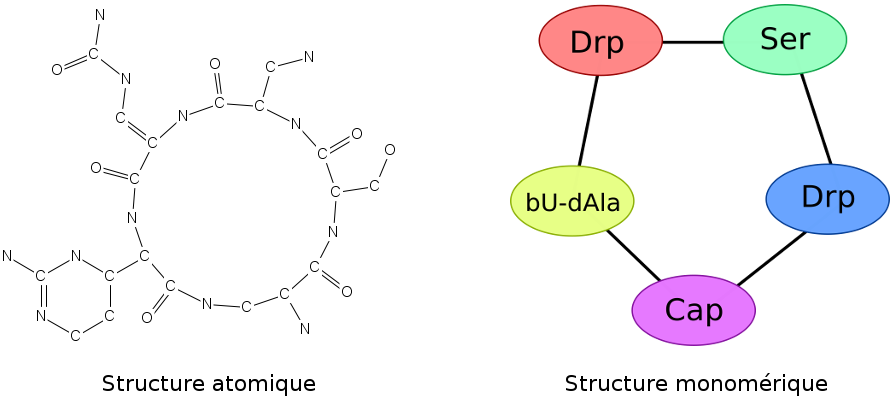
\includegraphics[width=400px]{Figures/s2m/Intro/structures.png}
    \caption{\label{structures}Structures atomique et monomérique de la Caprieomycin IIA.}
  \end{center}
\end{figure}

\paragraph{}Dans notre cas, nous allons partir des structures atomiques pour déduire les composants monomériques (voir figure \ref{structures}).
De telles structures sont présentes dans de nombreuses bases de données publiques, telles que PDB ou PubChem.
Il est possible de trouver au sein de ces bases de données de nombreuses structures atomiques de NRP dont on ne possède pas d'annotation monomérique facilement accessible.
Notre objectif sera d'être capable, pour toute structure moléculaire NRP, de déduire sa composition en monomères.
Ainsi, toutes les structures atomiques présentes dans les bases généralistes pourront être annotées et ajoutées à des bases spécialisées telles que Norine.
Ce type d'annotation pourra également être effectué sur toutes les nouvelles structures atomiques ajoutées.



\subsection{L'existant}

\paragraph{}Parmi l'existant, les logiciels CHUCKLES~\cite{siani_chuckles:_1994} et molBLOCKS~\cite{ghersi_molblocks:_2014} se démarquent des autres.
Dans les deux cas, les logiciels permettent, à partir d'une structure atomique d'un polymère, de trouver la structure monomérique.
Les deux logiciels sont opposés dans leur façon de prendre le problème.
CHUCKLES est constructif car il part des monomères pour reconstituer le polymère alors que molBLOCKS est destructif car il part du polymère pour retrouver les monomères par découpes successives de liens.
Nous allons ici présenter ces deux approches.


\subsubsection{CHUCKLES, une méthode constructive}

\paragraph{}CHUCKLES~\cite{siani_chuckles:_1994} est une méthode publiée en 1994 permettant de rechercher des peptides au sein d'une base de données.
Le but est de requêter une base de données de molécules en utilisant des expressions régulières représentant des sous-molécules d'intérêt.
Les recherches peuvent être effectuées à la fois au niveau atomique et au niveau monomérique.
Le but de CHUCKLES est de convertir rapidement les données du format monomérique vers le format atomique et inversement.
Les auteurs pensent qu'il est plus utile de conserver les formats atomiques en base plutôt que les séquences protéiques.
Sachant que la plupart des peptides de l'époque étaient déjà représentés par leur séquence, les auteurs proposent une méthode de transformation vers la structure atomique.
Cette transformation est appelée ``Forward-Translation'' (FT).

\begin{figure}[!ht]
  \begin{center}
    \includegraphics[width=450px]{Figures/s2m/formalisation/CHUCK_FT.png}
    \caption{\label{chuck_ft}CHUCKLES Forward Translation.
    Transformation des annotations peptidiques en SMILES.
    Sous l'annotation peptidique est écrite la formule SMILES après concaténation de tous les SMILES des monomères trouvés.
    Schémas issus de la publication}
  \end{center}
\end{figure}

\paragraph{}Pour mener à bien chaque ST, les auteurs ont besoin d'une table de transformation qui recense les structures atomiques de chacun des monomères à transformer.
Chaque structure ne doit pas contenir les atomes qui vont être perdus lors des liaisons avec d'autres monomères.
Pour les structures linéaires, la méthode propose une simple concaténation des structures atomiques selon la chaîne peptidique.
Lorsque les structures sont branchées ou cycliques, il est nécessaire d'ajouter dans la structure initiale l'information de liaison annexe.

Cette méthode de reconstruction des structures atomiques est très intéressante mais souffre du manque d'information des séquences protéiques.
On peut remarquer que la reconstruction ne peut fonctionner à tous les coups sans plus d'information.
En effet, si les monomères ne possèdent pas de groupement carboxyl et amine, la reconstruction ne peut pas être effectuée sans choix aléatoires d'orientation.

\begin{figure}[!ht]
  \begin{center}
    \includegraphics[width=300px]{Figures/s2m/formalisation/CHUCK_BT.png}
    \caption{\label{chuck_bt}CHUCKLES Backward Translation.
    La première partie représente la phase de recherche des monomères au sein de la structure atomique.
    La seconde partie représente la structure monomérique post contraction.
    On peut voir à gauche la chaîne principale qui a été extraite à partir du N initial.
    A droite sont répertoriés les deux ponts disulfure extraits hors de la chaîne principale.
    Chaque monomère découvert comporte un identifiant différent de son nom pour éviter d'avoir deux fois le même nom comme cela pourrait être le cas ici.
    Schémas issus de la publication}
  \end{center}
\end{figure}

\paragraph{}La seconde partie de la méthode présente la transformation inverse (``Backward-Transformation'' (BT)).
C'est cette partie qui est très intéressante pour l'annotation car elle part des structures atomiques pour reconstruire les structures monomériques.
Les auteurs proposent une annotation en deux temps.
Le premier temps représente la phase de recherche des monomères et le second temps la conversion des monomères trouvés en une annotation.
L'idée de la première phase est de rechercher chaque monomère connu en masquant les atomes déjà utilisés par des monomères précédemment trouvés.
En recherchant les monomères par nombre d'atomes décroissant, les auteurs s'assurent que de petits monomères ne viendront pas prendre la place de plus gros.
Lors de la seconde phase, les atomes des molécules sont contractés pour ne plus former qu'un seul n\oe{}ud par monomère.
Le N terminal de la chaîne peptidique est ensuite recherché afin d'extraire l'annotation de cette chaîne en suivant les liaisons peptidiques.
Enfin, les liaisons n'ayant pas encore été explorées sont ajoutées à la représentation monomérique finale.

Comme pour le FT, le BT utilise des techniques intelligentes mais encore faillibles.
Dans le cas des NRP, certains monomères ne possèdent pas les deux domaines pour les liaisons peptidiques.
Il est donc potentiellement impossible de retrouver une chaîne principale.
De plus, lors de la recherche, si les monomères à rechercher sont structurellement proches, il est possible qu'un gros monomère vienne prendre la place d'un plus petit en débordant sur un ou plusieurs monomères voisins.
Dans ce cas, vu qu'aucun retour en arrière n'est effectué, l'annotation sera inexacte voir incomplète.


\subsubsection{molBLOCKS, une méthode destructive}

\begin{figure}[!ht]
  \begin{center}
    \includegraphics[width=400px]{Figures/s2m/Intro/molBlocks.png}
    \caption{\label{molBlocks}Application de la méthode molBlocks sur le polymère ACV.
    Le polymère est séparé en morceau par une règle de liaison peptidique.
    Les trois morceaux correspondent aux trois monomères réellement inclus, la découpe fonctionne.}
  \end{center}
\end{figure}

\paragraph{}Le logiciel molBLOCKS~\cite{ghersi_molblocks:_2014} n'est à la base pas conçu pour le travail que nous cherchons à effectuer.
C'est un logiciel qui permet de découvrir des monomères en repérant les sous morceaux fréquents au sein d'une population de polymères.
Pour cela le logiciel découpe les polymères en petits morceaux et effectue des comptages sur ces morceaux.
Ces découpes suivent des règles entrées par l'utilisateur.
Par exemple en donnant comme règle
\begin{chemmath}
  O=CNH \longrightarrow C=O + NH
\end{chemmath}
toutes les liaisons peptidiques seront ciblées et déconnectées (voir figure \ref{molBlocks}).
Pour des protéines ribosomiques, la découpe sera donc parfaite avec cette seule règle et les monomères seront découverts.

\begin{figure}[!ht]
  \begin{center}
    \includegraphics[width=300px]{Figures/s2m/Intro/molBlocks_problem.png}
    \caption{\label{molBlocks_problem}Dans le cas de ce di-peptide, un sucre est lié à une Hydroxy-Phenil-Glycine (Hpg).
    En utilisant la règle de découpe à appliquer pour les hydroxyl, une ambigüité et une erreur apparaissent.
    Nous ne pouvons savoir de quel côté les découpes vont être les plus pertinentes avant d'essayer de reconnaître les monomères.
    De ce fait, 4 découpes différentes sont possibles.
    De plus, le cycle du sucre se voit ouvert alors que la découpe est inutile.}
  \end{center}
\end{figure}

\paragraph{}Dans notre cas, nous pourrions utiliser un tel logiciel pour découper les NRP en monomères.
En effectuant par la suite une étape de reconnaissance de ces monomères, il serait alors possible de reconstruire le peptide.
Cependant, certaines réactions effectuées au sein des NRP ne permettent pas de découper entièrement le peptide avec la seule règle énoncée précédemment.
Toutes les liaisons non peptidiques énoncées au chapitre précédent ne seront pas découpées.
Il est donc nécessaire de rajouter nombre de nouvelles règles.
Cependant, la liaison hydroxyl à elle seule ne permet déjà plus d'effectuer une découpe correcte.
Pour pouvoir la délier, il faudrait une règle du type
\begin{chemmath}
  COC \longrightarrow CO + C
\end{chemmath}
Mais ce genre de règle est ambigu.
Comment savoir de quel côté du O la liaison doit être rompue ?
De plus, certains monomères comme le glucose sont initialement composés de $COC$.
Ces monomères seront donc découpés alors qu'ils ne devraient pas l'être.
Pour ces deux raisons, nous ne pourrons pas directement utiliser ce logiciel afin de convertir nos structures atomiques en structures monomériques.


\subsubsection{Vue générale}

\paragraph{}En dehors des deux logiciels que nous venons de présenter, rien n'est dédié spécifiquement à la tâche que nous cherchons à accomplir.
Un grand nombre de techniques que j'ai étudiées ne permettent que la résolution de sous problèmes.
Par exemple, lors de la présentation de CHUCKLES, nous citons une implémentation des SMARTS appelée AMBIT-SMARTS.
Les SMARTS sont des expressions régulières moléculaires qui permettent de définir des motifs à rechercher.
En appliquant un SMARTS sur une molécule (comme le permet AMBIT-SMARTS), nous pouvons savoir si cette molécule contient ce motif.
Ce type de technique permet de savoir si une molécule est contenue dans une autre, ce qui dans notre cas reviendrait à savoir si un monomère est contenu dans un polymère.
Cette tâche très importante n'est pas suffisante pour répondre à nos attentes, mais peut éventuellement faire partie des sous techniques à utiliser.




\subsection{Vers des problèmes informatiques}

\paragraph{}Pour concevoir notre logiciel d'annotation, nous allons nous inspirer des techniques existantes en essayant de dépasser leurs difficultés.
Nous possédons, au sein de Norine, une grande base de connaissances de monomères existants (plus de 500) et nous pouvons nous appuyer sur cette base bien établie pour assurer l'existence des monomères lors des annotations.
Cette base étant, essayons de concevoir un algorithme constructif.


\subsubsection{Une histoire de sous problèmes}

\paragraph{}L'algorithme CHUCKLES tire partie de la différence entre les 20 acides aminés pour se permettre de rechercher les plus gros en premier et de ne jamais revenir sur les choix faits.
Rechercher les monomères par taille (en nombre d'atomes) décroissante et en masquant les atomes déjà utilisés est un choix pertinent car il permet d'éviter de reconnaître partout les petits acides aminés.
Dans notre cas, la proximité entre certains monomères ne nous permettra pas de les départager grâce à un tri par taille.
Il sera nécessaire de modifier les solutions incomplètes pour essayer de les améliorer.
Contrairement à CHUCKLES, nous aurons donc besoin de connaître les différents monomères candidats à la composition du polymère même lorsqu'ils sont chevauchants à des monomères déjà placés.
Si d'un côté nous recherchons les monomères au sein du NRP puis de l'autre nous assemblons ceux trouvés, alors nous pouvons séparer notre programme en deux sous-problèmes complètement distincts.

\begin{figure}[!ht]
  \begin{center}
    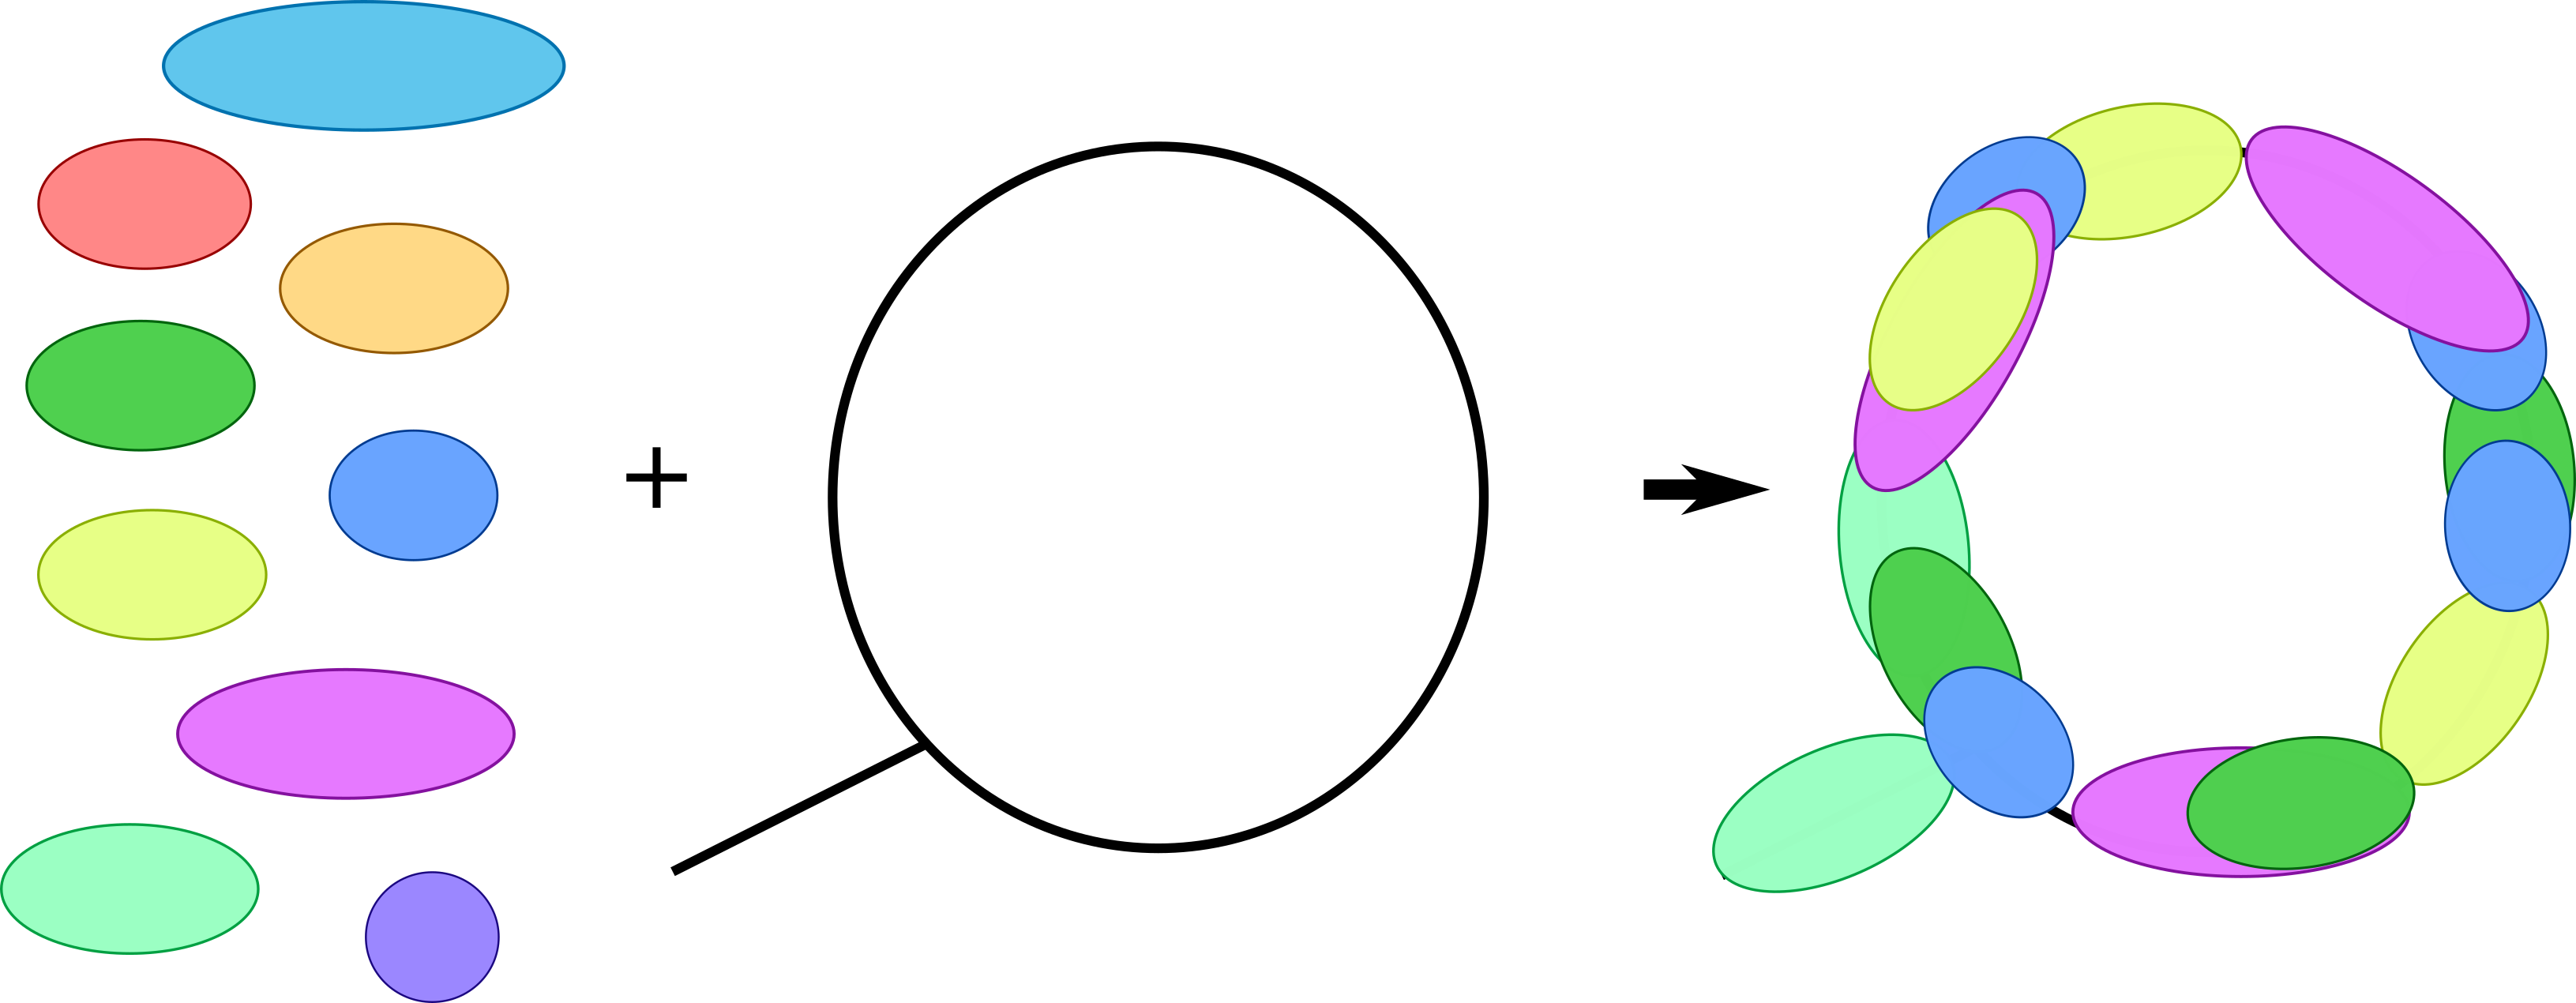
\includegraphics[width=400px]{Figures/s2m/Intro/searching.png}
    \caption{\label{search_fig}Première étape : Recherche des monomères (ellipses colorées) sur le peptide à annoter (cycle noir branché).}
  \end{center}
\end{figure}

\paragraph{}Dans un premier temps, nous allons chercher à déterminer quels sont les monomères qui pourraient composer le peptide étudié.
En utilisant la base Norine, nous pouvons indépendamment rechercher chacun des monomères connus au sein de la molécule à annoter.
La recherche exacte d'un monomère au sein d'un peptide est donc notre premier sous problème à résoudre.
Ce sous problème sera appelé la ``recherche'' (voir figure \ref{search_fig}).

\begin{figure}[!ht]
  \begin{center}
    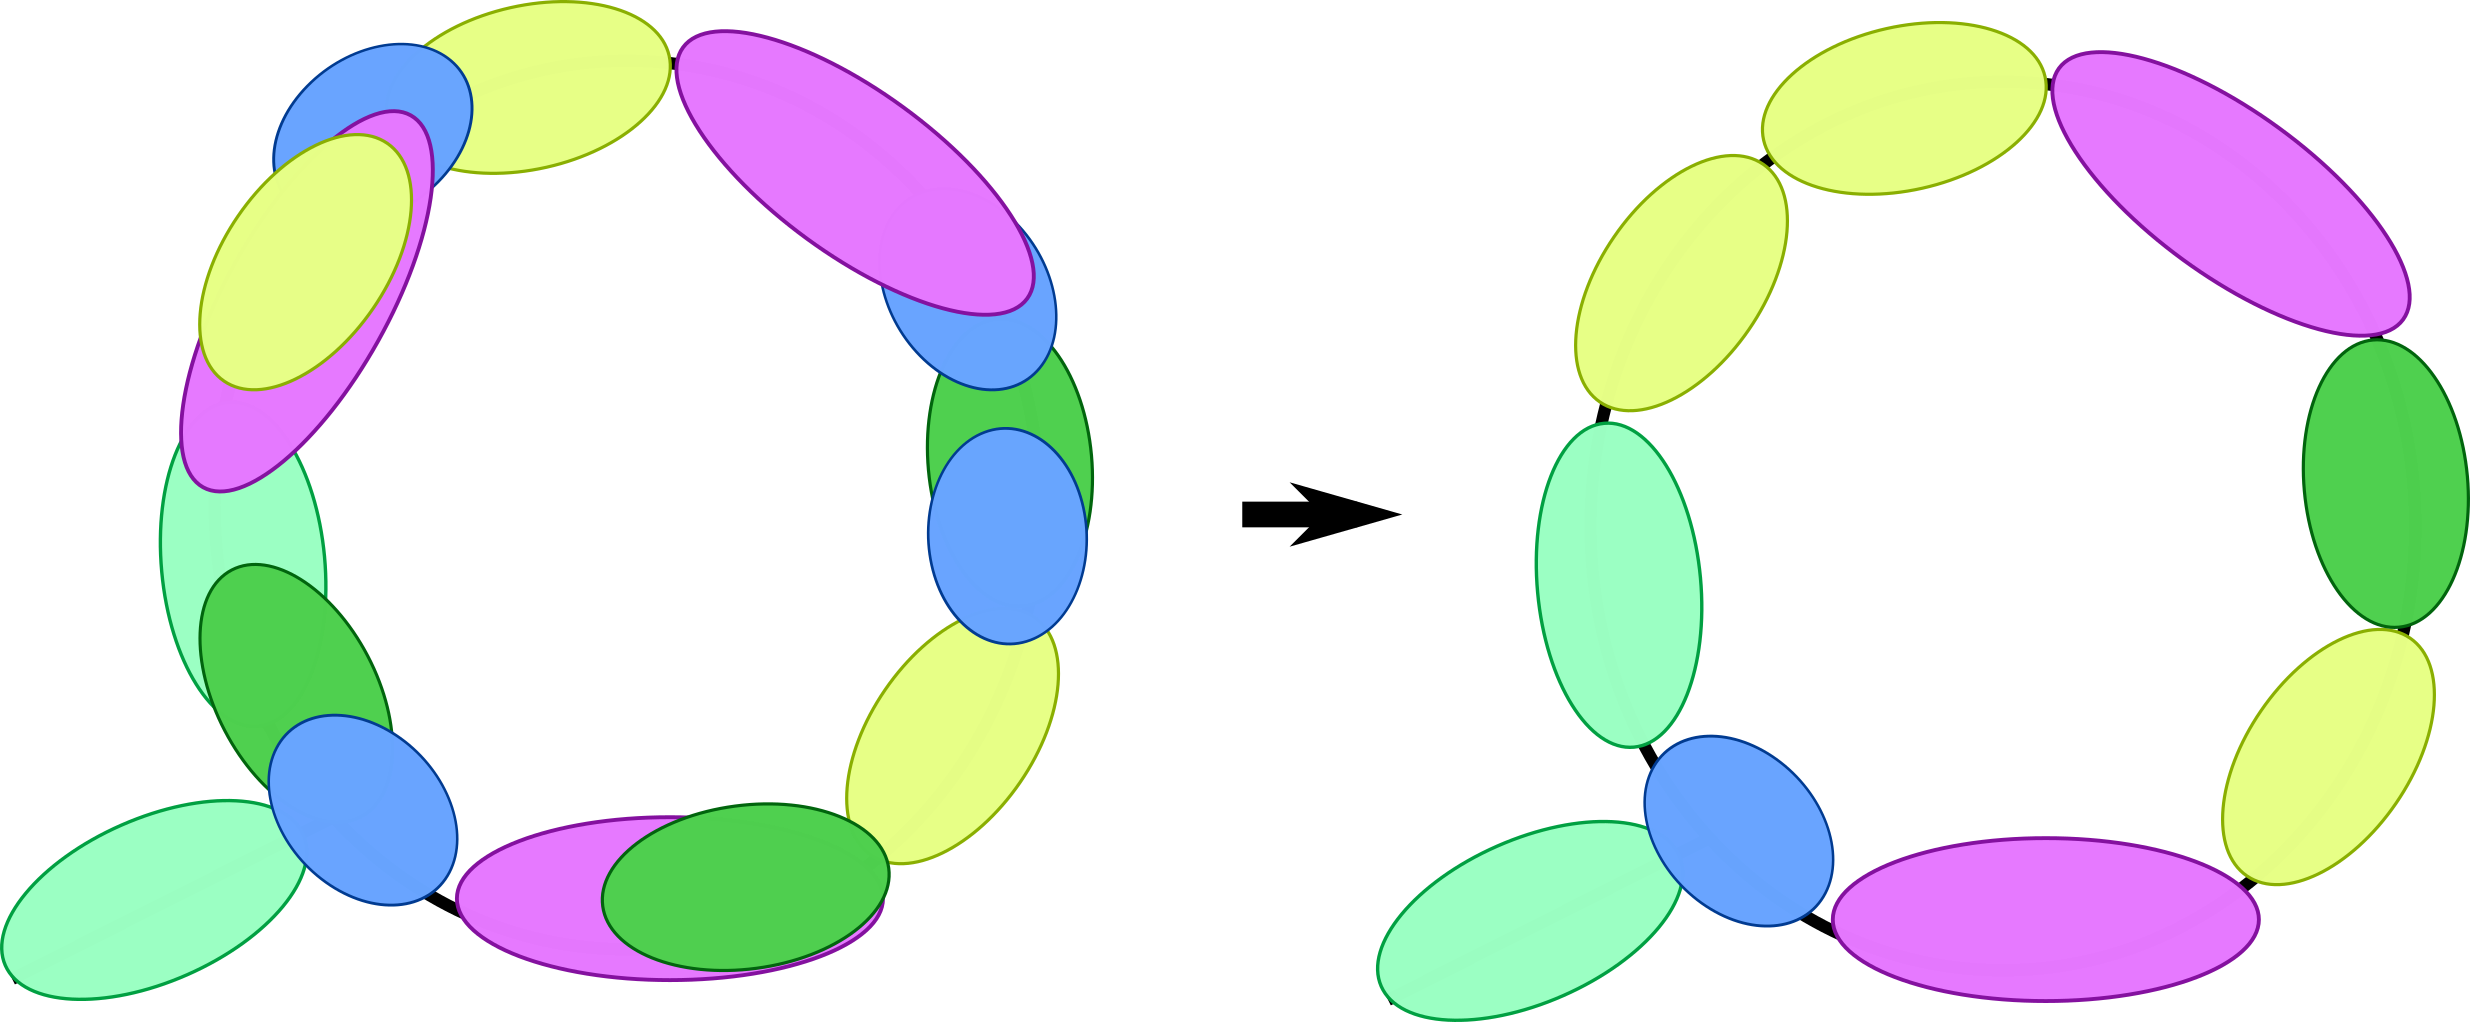
\includegraphics[width=400px]{Figures/s2m/Intro/tiling.png}
    \caption{\label{tiling_fig}Seconde étape : Sélection des monomères parmi ceux trouvés à l'étape 1.
    Le but est d'obtenir une structure monomérique non chevauchante de couverture maximale.}
  \end{center}
\end{figure}

\paragraph{}Dans un second temps, nous devrons choisir parmi tous les monomères candidats issus de la recherche, lesquels composent réellement le polymère.
Nous aurons plusieurs contraintes associées à ce problème.
Aucun des monomères choisis dans la solution ne peux être chevauchant avec un autre.
En effet, aucun atome ne peut provenir de deux molécules différentes et donc aucune sous partie de monomères ne peut être chevauchante avec un autre monomère.
De plus nous allons chercher à obtenir une annotation complète des peptides, ce qui correspond à maximiser les atomes du polymère couvert par des monomères.
On appellera cette étape l'étape de ``pavage'' (voir figure \ref{tiling_fig}).

\subsubsection{Des molécules aux graphes}

\newtheorem{definition}{Definition}
\begin{definition}\textbf{Graphe :}
 Un graphe est une représentation mathématique d'un ensemble d'objets où chacun des objets est appelé un sommet et
 chaque relation entre deux objets est représentée par un lien entre les deux sommets correspondants.
 On appéllera arité d'un noeud dans un graphe, le nombre de liens connectés à ce noeud.
\end{definition}

\paragraph{}En informatique, les graphes sont utilisés pour représenter de nombreuses données.
Dans notre cas, les molécules peuvent être représentées comme des graphes étiquetés et non orientés.
Un atome est alors un n\oe{}ud dont l'étiquette est le nom de l'atome.
Une liaison chimique est une arête du graphe.
La structure monomérique peut elle aussi être représentée sous forme de graphe.
Dans ce cas, les n\oe{}uds sont les monomères et leurs étiquettes sont leurs noms.
Les arêtes sont les liaisons formées entre les monomères pour construire le peptide.
Passer du graphe atomique au graphe monomérique revient donc à une contraction de n\oe{}uds.


\subsubsection{Formalisation en problèmes de graphes}

\paragraph{}Comme expliqué plus haut le problème de recherche de sous composants d'un polymère peut être divisé en deux
plus petit problèmes : un problème de recherche de monomères et un problème de placement des monomères trouvés. Traitons
donc séparément ces deux problèmes.

\paragraph{Recherche de monomères}Rechercher un monomère dans un polymère revient à rechercher un petit graphe atomique
$S$ dans un plus gros graphe $G$. Deux cas sont alors possibles : soit nous cherchons à trouver exactement $S$ dans
$G$, soit nous cherchons une approximation de $S$ dans $G$. Dans le premier cas, nous allons nous intéresser à l'
``Isomorphisme de Sous-graphe'' (en anglais Subgraph Isomorphism (SI)). Dans le second cas, nous nous intéresserons au
``Sous-graphe Maximum Commun'' (en anglais Maximum Common Subgraph (MCS)). Les recherches de SI ou de MCS ont toutes
deux été prouvées NP-Complet mais, pour chacun des problème, il existe des algorithmes rapides en pratique pour des graphes
aux propriétés particulières dont nous parlerons dans la sous-partie suivante.

\paragraph{Placements des monomères}Une fois les monomères détectés, il est nécessaire de prendre une décision pour les parties du polymère où plusieurs d'entre eux ont été détectés au même endroit.
L'objectif est donc de faire un choix entre les différents morceaux possibles afin de chercher à ne garder que les pièces non chevauchantes qui permettent de couvrir au mieux le polymère (Si possible totalement).
Ce genre de méthode est appelée pavage sans recouvrement.
Cette étape donnant accès à un lien direct entre atomes et monomères, une étape de contraction de graphe permettra d'obtenir le graphe monomérique.




\section{Isomorphisme de Sous-graphe vs Sous-graphe Maximum Commun}

\paragraph{}Nous venons de voir que la recherche de monomères pouvait correspondre à deux problèmes différents en recherche de graphe.
Formalisons et étudions ici ces deux problèmes afin de choisir celui qui nous utiliserons au sein de notre logiciel d'annotations.
Voyons les différentes façons de les résoudre ainsi que les forces et faiblesses de ces approches.


\subsection{Sous-graphe Maximum Commun}

\subsubsection{Définition}

\begin{figure}[!ht]
  \begin{center}
    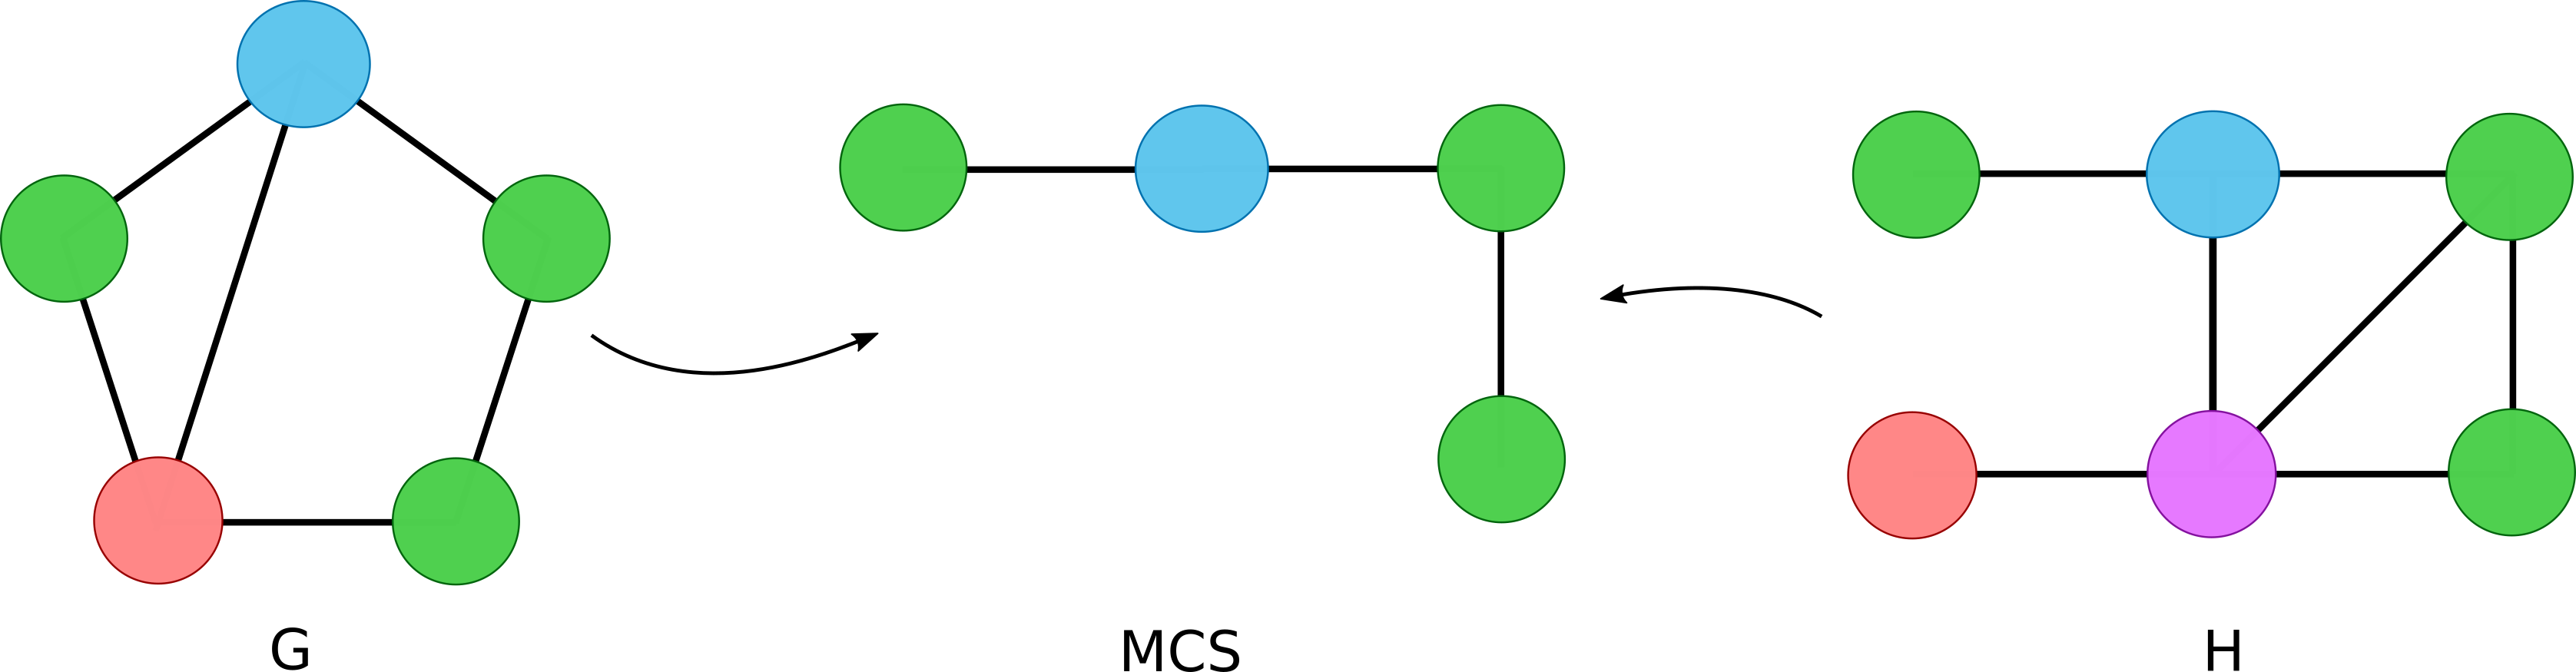
\includegraphics[width=450px]{Figures/s2m/MCS-SI/mcs.png}
    \caption{\label{mcs_fig}MCS obtenu à partir des graphes G et H.
    Le MCS obtenu n'est pas connexe du fait des liens vers le n\oe{}ud rouge, qui ne sont pas les mêmes dans G et H.}
  \end{center}
\end{figure}

\paragraph{}Commençons par définir précisément le problème du MCS.
Comme le nom l'indique, le problème du MCS est un problème de recherche de la sous partie commune maximale entre deux graphes (Voir figure \ref{mcs_fig}).
C'est à dire trouver un ensemble de n\oe{}uds présents dans les deux graphes.
Il faut non seulement que les n\oe{}uds partagent les même étiquettes mais également les mêmes voisins.
Si deux n\oe{}uds ont la même étiquette mais ne partagent pas les mêmes voisins dans les deux graphes, alors ils ne font pas partie du MCS.
C'est par exemple le cas du n\oe{}ud rouge au sein de la figure.
Le problème de recherche de sous graphe commun connexe maximal (MCCS) est un problème encore plus difficile car il impose de fortes contraintes supplémentaires.
Le problème du MCS à été prouvé NP-Complet\cite{garey_computers_1979}, ce qui empêche (en tout cas pour le moment) l'émergence d'algorithmes de résolution polynomiaux efficaces.

\paragraph{}Dans notre cas, nous pouvons effectuer une réduction vers ce problème pour la recherche des monomères.
Si l'on considère qu'un monomère et un polymère sont des graphes atomiques, alors trouver une sous partie commune à ces deux graphes revient à trouver un endroit où un morceau du monomère est retrouvé dans le peptide.
En imposant que le graphe commun soit d'une taille minimale fixée, nous pourrons éviter d'avoir des résultats ne contenant que quelques atomes par hasard.

\paragraph{}Du fait de la NP-complétude du problème, trouver des solutions est très compliqué.
Il existe tout de même quelques algorithmes de résolution exacts mais la majorité des articles à propos de MCS traitent d'heuristiques de résolution rapide.
Voyons ensemble ces deux catégories d'algorithmes en s'appuyant sur les reviews~\cite{raymond_maximum_2002, ehrlich_maximum_2011}.


\subsubsection{Les méthodes exactes de résolution}

\paragraph{}Au sein des algorithmes de résolution exacte du MCS, il existe deux grandes écoles.
D'un côté, le problème du MCS est réduit en un problème de clique maximale avant d'utiliser des solveurs de ce second problème.
D'un autre côté, les méthodes de résolution se basent sur des méthodes de backtracking.



\paragraph{La réduction en clique maximale}
Il est possible de réduire le problème MCS en un problème de résolution de clique maximale~\cite{pelillo_matching_1999,grosso_simple_2008,rahman_small_2009}.
Une clique est un ensemble de n\oe{}uds dans un graphe tel que tous les n\oe{}uds de cet ensemble sont reliés entre eux.
Rechercher la clique maximale revient à rechercher le sous ensemble maximal de n\oe{}uds d'un graphe pour lequel tous les n\oe{}uds sont liés les uns aux autres.
Il est possible d'obtenir plusieurs cliques maximales dans un même graphe.
Ce problème est également NP-Complet~\cite{akkoyunlu_enumeration_1973}.
Les résolutions de ce problème sont toutes des dérivées de la recherche exhaustive par backtracking.
Il est possible de ne pas passer par toutes les combinaisons possibles en réduisant l'espace de recherche en fonction de l'arité des n\oe{}uds ou de leur contexte local mais les algorithmes restent exponentiels~\cite{tomita_worst-case_2004}.

\begin{figure}[!ht]
  \begin{center}
    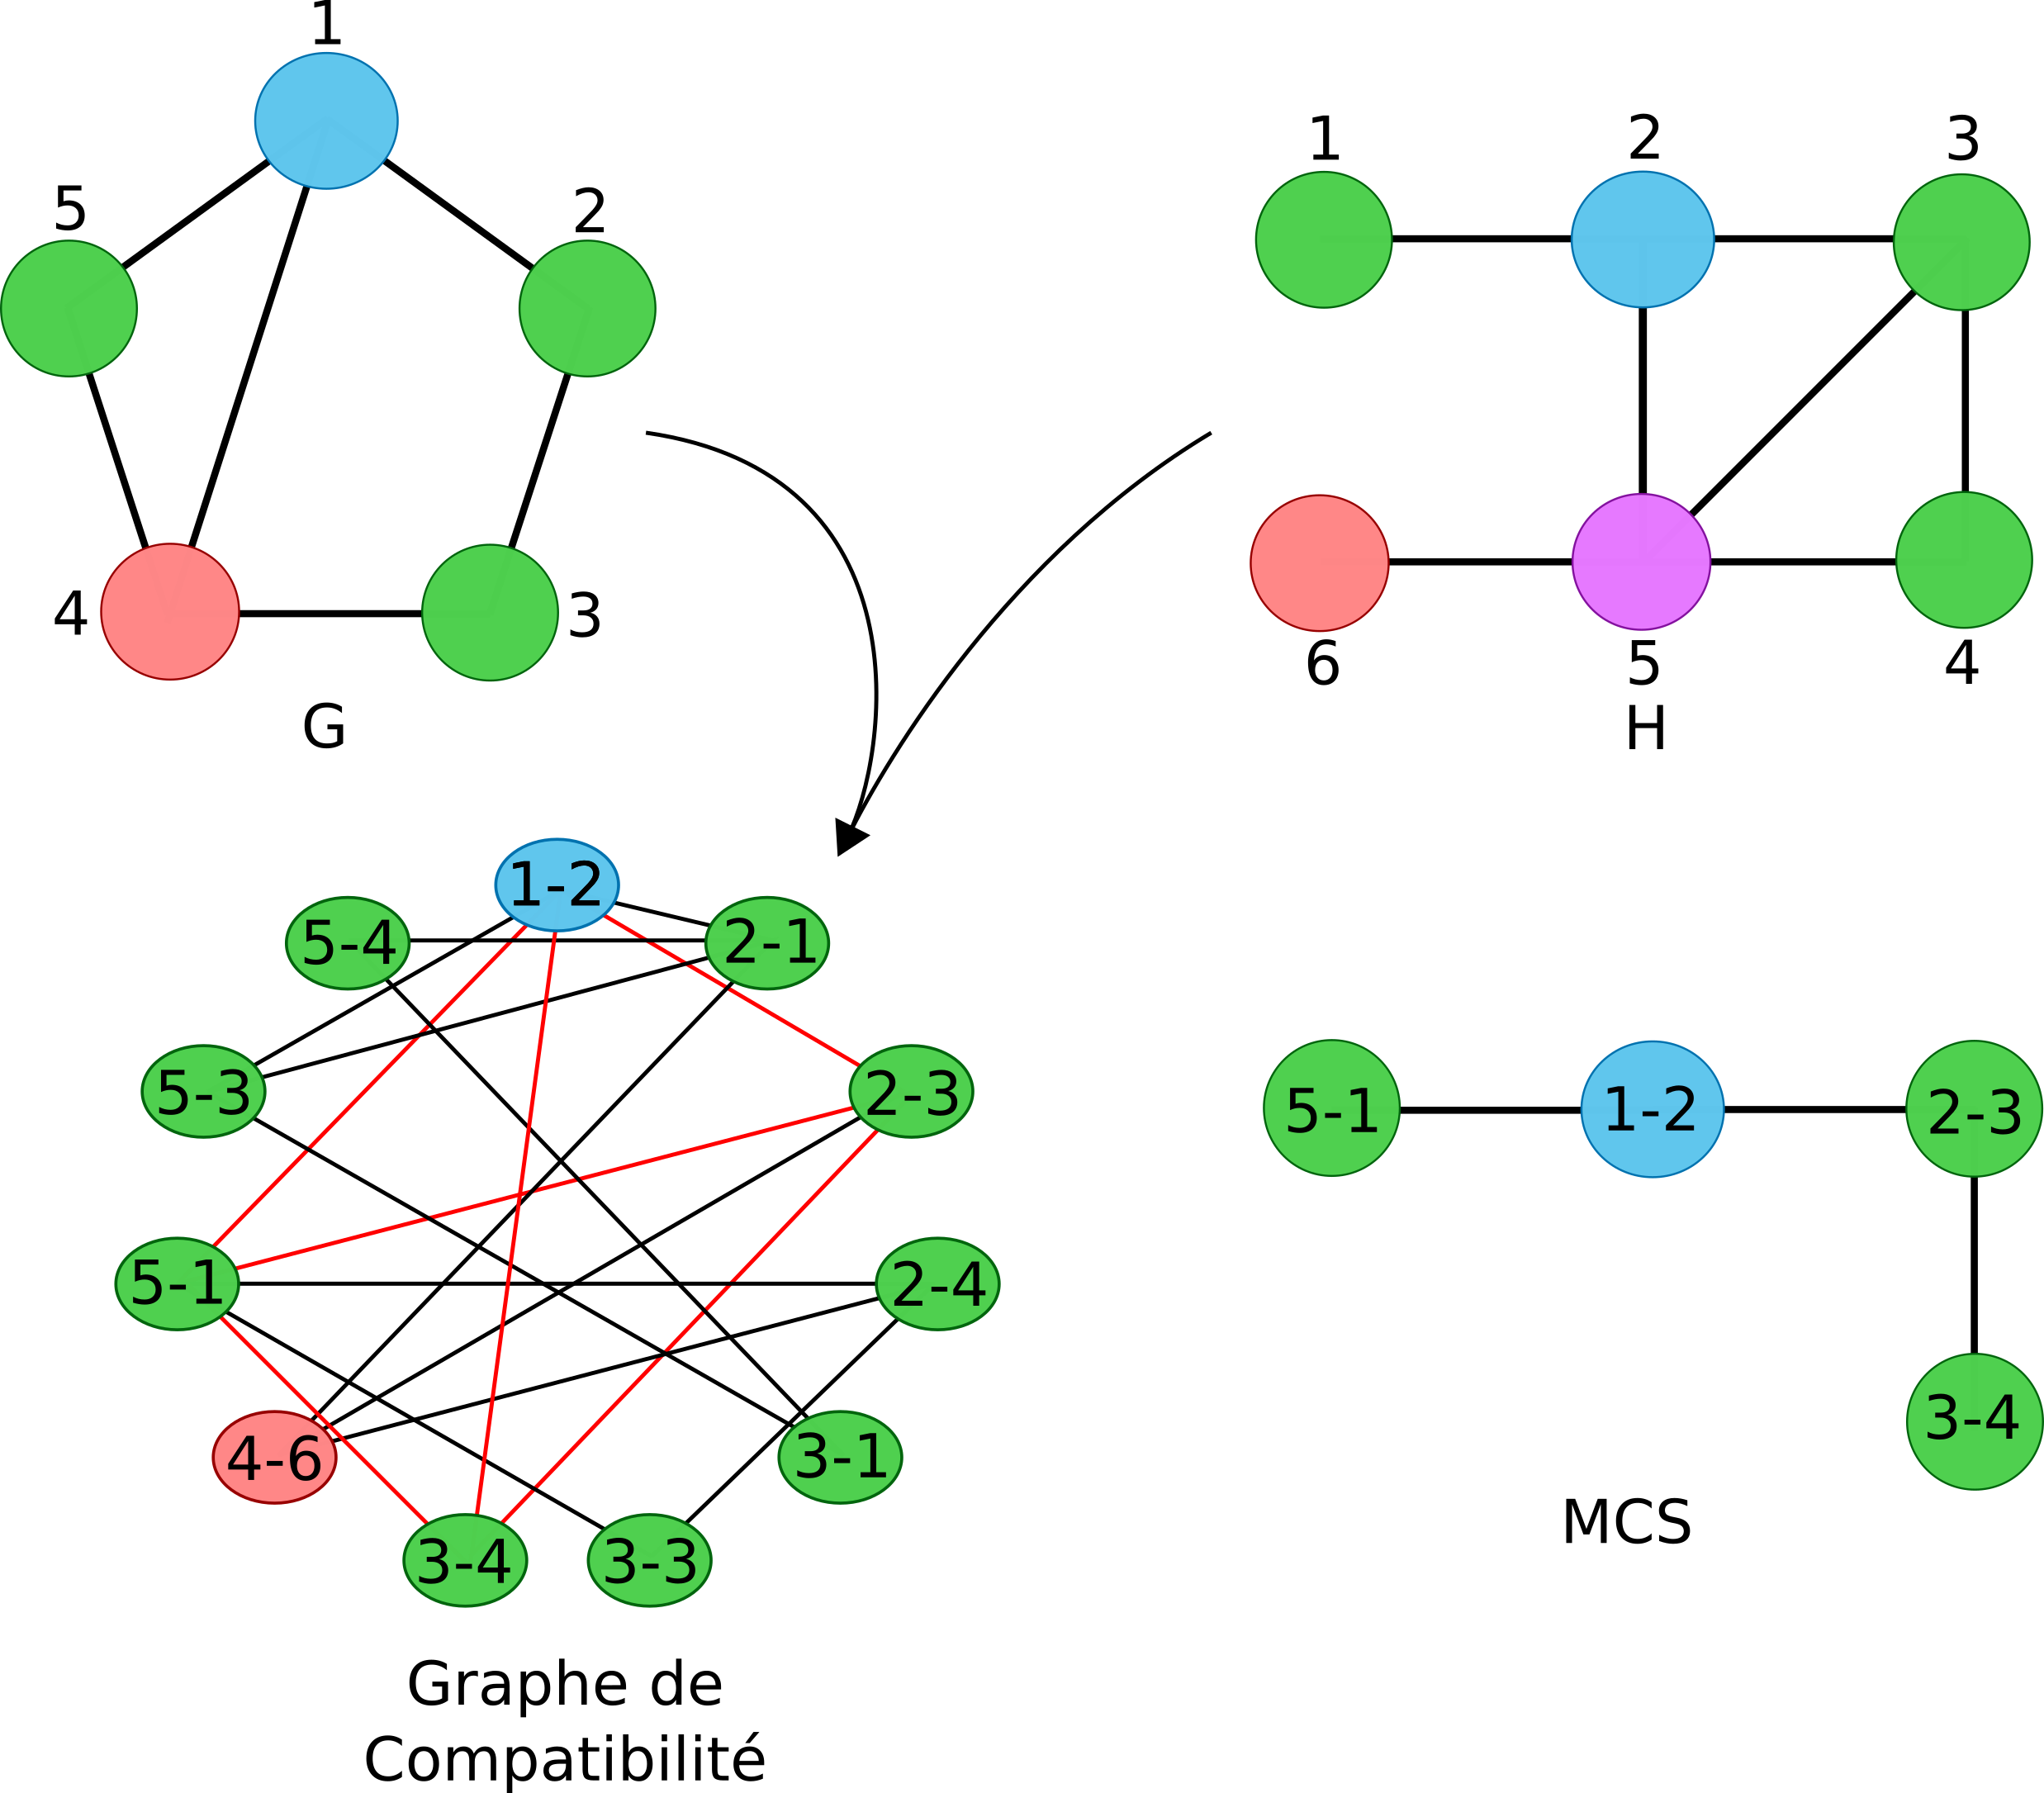
\includegraphics[width=400px]{Figures/s2m/MCS-SI/clique_solve.png}
    \caption{\label{clique_solve_fig}Résolution d'un MCS par réduction en clique maximale.
    Les couleurs représentent les étiquettes des noeuds.
    Dans le graphe de compatibilité les arêtes rouges identifient la clique maximale détectée.}
  \end{center}
\end{figure}

\paragraph{}Pour obtenir un MCS à partir de solveur de clique maximale, il est nécessaire de construire un graphe de compatibilité (voir schéma \ref{clique_solve_fig}).
Un graphe de compatibilité (GC) est un graphe créé à partir du croisement des deux graphes (qu'on appellera G et H).
Pour les n\oe{}uds du GC, on génère tous les couples $(x, y)$ possibles avec $x$ issu de G et $y$ de H et dont les étiquettes sont identiques.
Ensuite on ajoute un lien entre deux couples $(x_1 , y_1)$ et $(x_2 , y_2)$ de GC si $x_1$ est voisin de $x_2$ dans G et $y_1$ voisin de $y_2$ dans H.
On ajoute également un lien si les $x$ sont non voisins et les $y$ également.
En résolvant le problème de clique maximale sur le GC, on obtient le MCS.


\begin{figure}[!ht]
  \begin{center}
    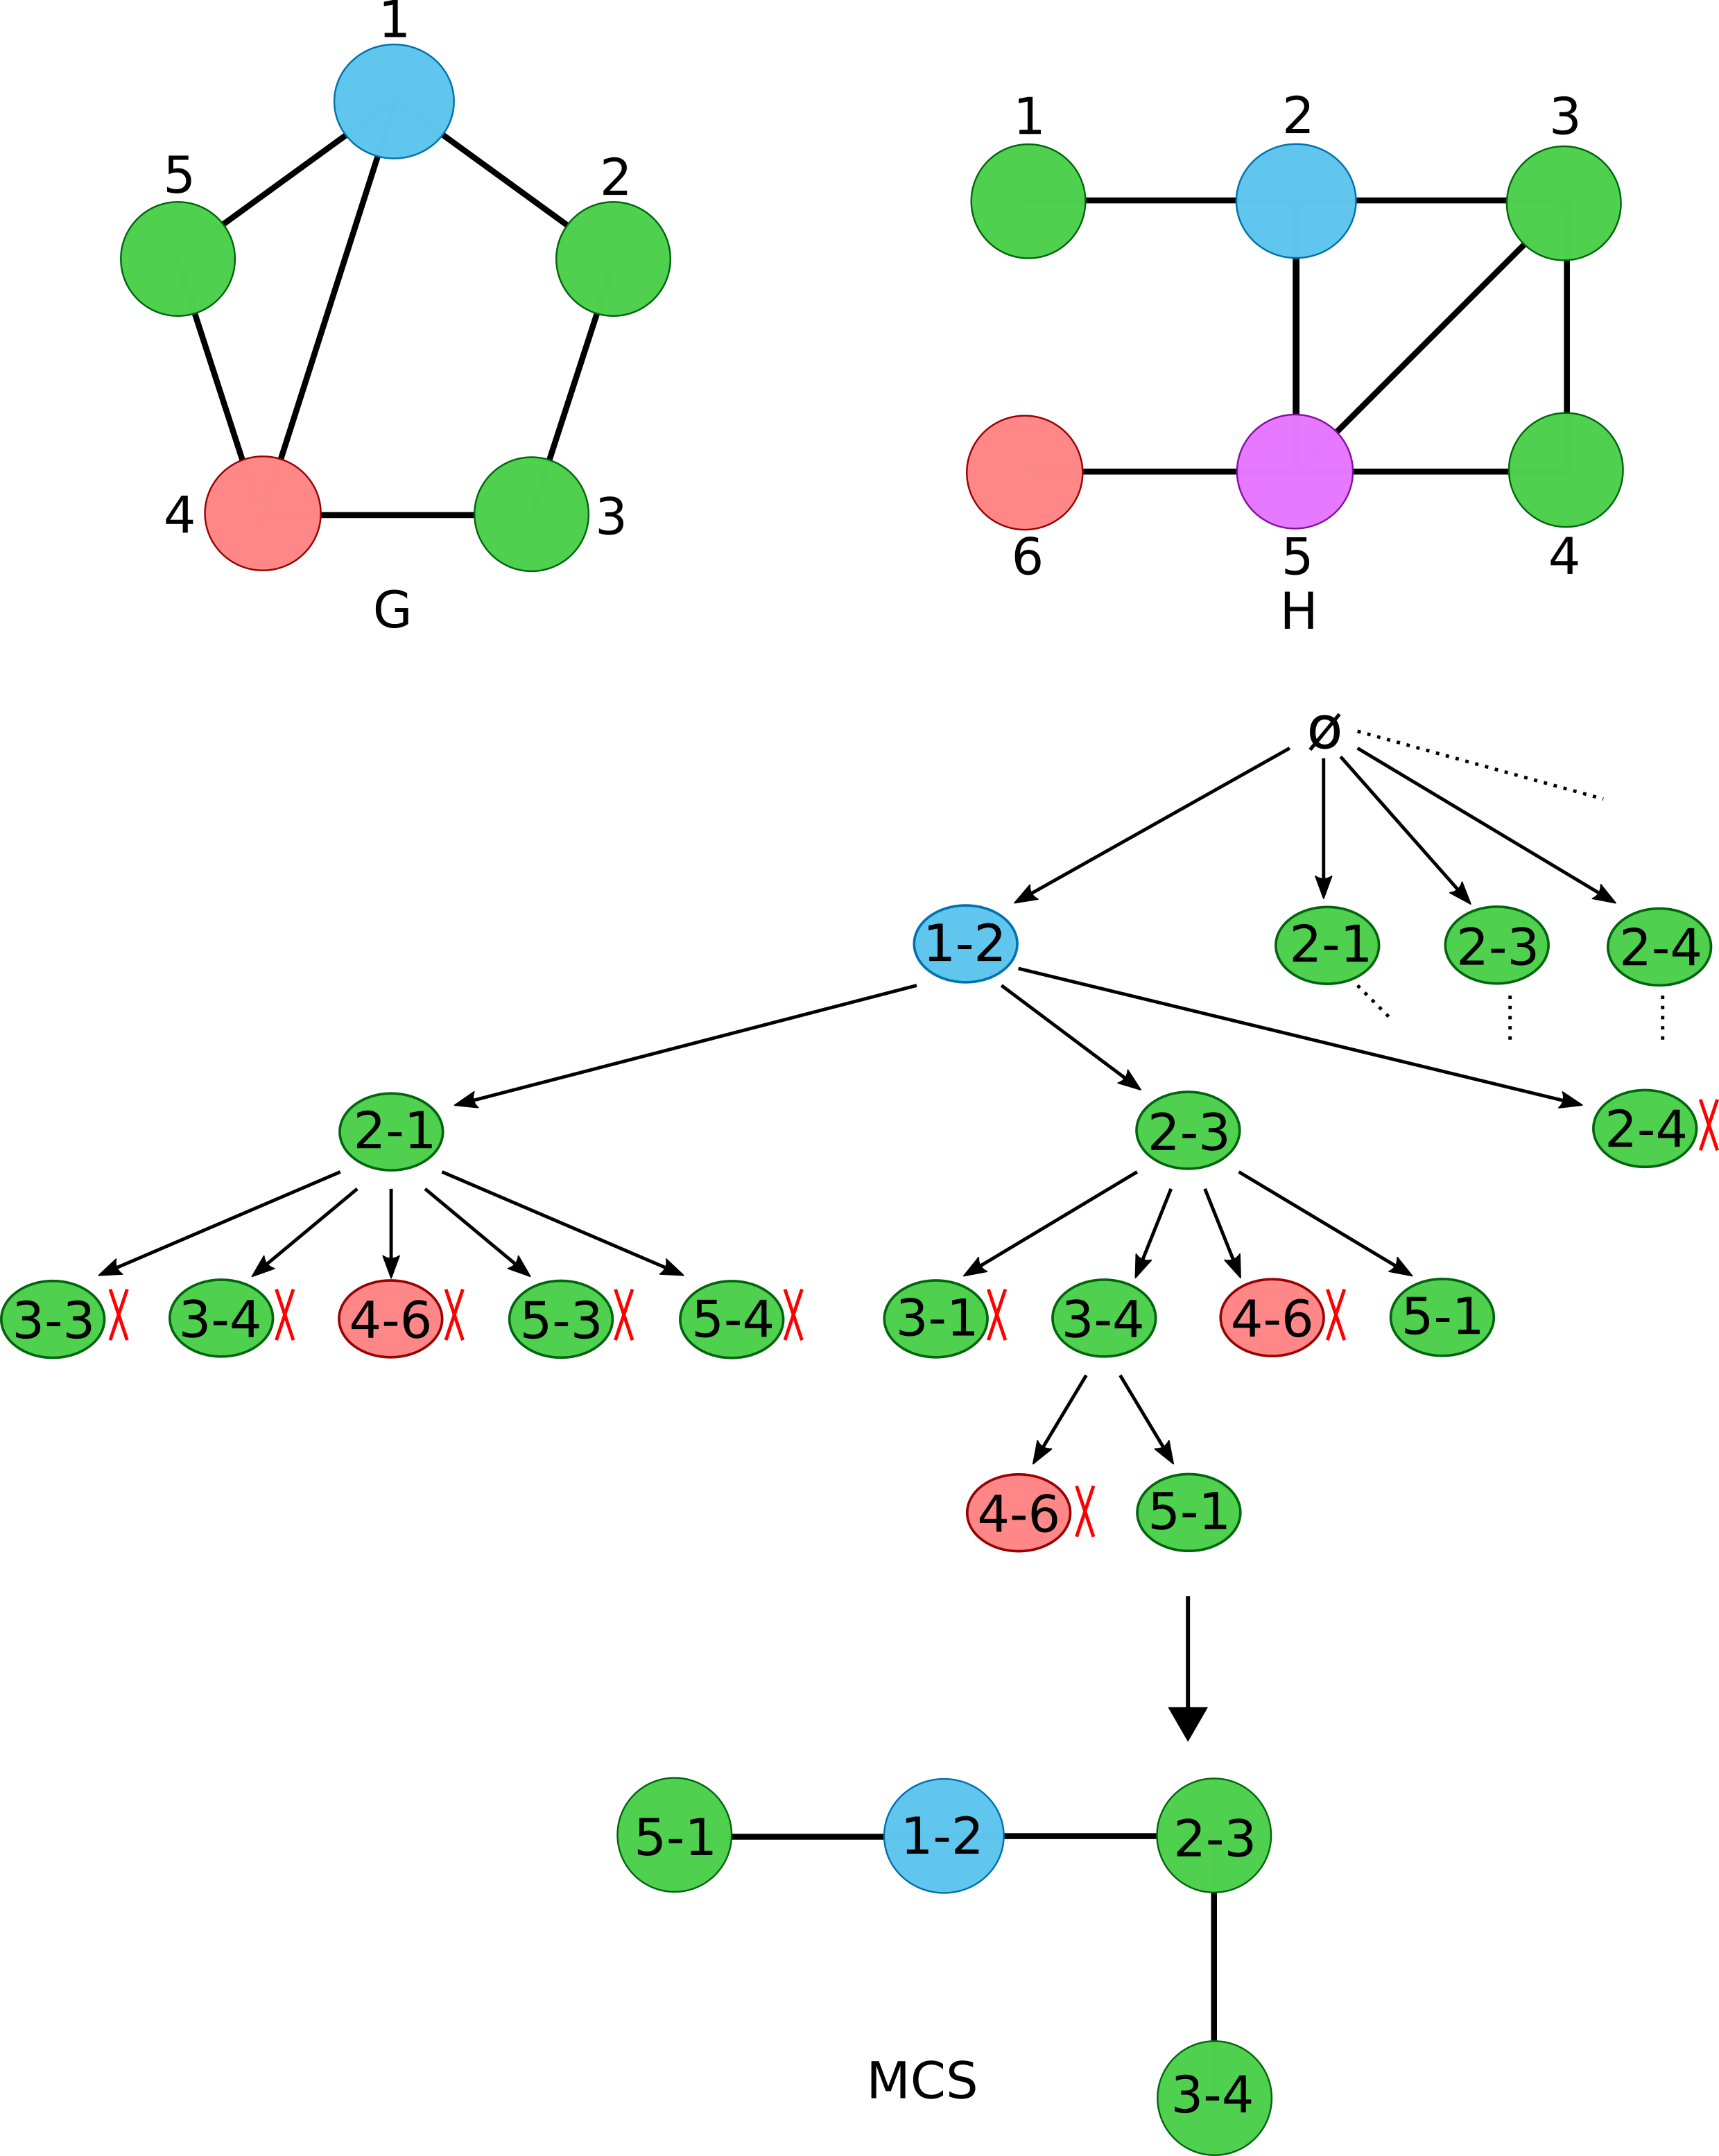
\includegraphics[width=400px]{Figures/s2m/MCS-SI/backtracking_solve.png}
    \caption{\label{backtracking_solve}Exemple de résolution de MCS par un backtracking naïf.
    L'arbre part d'une bijection vide et ajoute un couple à chaque étape.
    Parfois l'algorithme tombe sur un couple compatible mais dont les voisins ne sont pas le bijection.
    La solution est alors rejetée (croix rouge).
    La solution est trouvée par l'ensemble des chemins qui mènent aux feuilles valides les plus profondes dans l'arbre.}
  \end{center}
\end{figure}


\paragraph{Recherche par Backtracking}
La majorité des algorithmes exacts effectuent des recherches via des méthodes de backtracking~\cite{manic_branch&cut_2009,mcgregor_backtrack_1982,kawabata_build-up_2011}.
Un MCS est une bijection entre deux sous ensembles de n\oe{}uds dans deux graphes distincts.
Les méthodes de backtrack effectuent une reconstruction itérative de cette bijection.
Les couples de n\oe{}uds compatibles, n'étant pas encore présents au sein de la bijection, sont ajoutés un à un (voir figure \ref{backtracking_solve}).
Lorsque l'algorithme arrive dans une impasse (plus aucune possibilité d'ajouter un couple), il revient en arrière sur une association puis fait un choix différent.
En sauvegardant l'ensemble qui a contenu le plus de n\oe{}uds, on obtient la clique maximale après le parcours de tout l'arbre des possibilités.
Encore une fois, certaines des techniques citées permettent des accélérations pratiques en coupant des branches de recherche mais jamais l'ordre de grandeur de la complexité n'est changé.
Dans le cas des MCCS, il faut obliger une contrainte supplémentaire d'ajout de couple au sein de la bijection~\cite{chang_moderately_2014}.
Chacun des n\oe{}uds du couple à ajouter doit être voisin de l'un des n\oe{}uds d'un même couple précédemment inclus dans la bijection.

\paragraph{}Il existe bien d'autres méthodes exactes pour résoudre des MCS pour des graphes particuliers.
Cependant, aucun de ces cas particuliers ne correspond à la réalité des molécules que nous allons traiter.
Nous ne détaillerons donc pas celles-ci ici.


\subsubsection{Les méthodes heuristiques}

\paragraph{}Il existe une très grande quantité d'heuristiques de résolution du MCS.
La méthode qui revient le plus souvent est une méthode de recherche par similarités locales~\cite{yan_substructure_2005,willett_similarity_2011}.
Ce sont des algorithmes utilisés au sein de bases de données pour rechercher des structures chimiques par ressemblance avec une requête.
Chaque molécule de la base est décomposée en un grand nombre de critères topologiques locaux.
Ces critères sont entrés dans un vecteur appelé fingerprint.
Lors d'une requête, le motif recherché est à son tour transformé en fingerprint et une mesure de similarité est effectuée avec les vecteurs présents en base.
Les fingerprints les plus proches (fonction de score selon les méthodes~\cite{maggiora_molecular_2011,ndiaye_cp_2011}) sont déclarés en possession d'une sous partie commune.
Cette méthode ne donne aucune assurance quant à l'obtention de réels MCS.
C'est la rapidité d'exécution de l'algorithme qui est recherchée.
Dans notre cas, cette méthode est innappropriée puisque nous cherchons de vrais MCS.

\paragraph{}D'autres méthodes sont plus proches des méthodes exactes par recherche backtracking~\cite{grosso_simple_2008, wang_fmcsr:_2013}.
Ici, les auteurs construisent plusieurs bijections en parallèle.
La différence avec les méthodes exactes est qu'ils ne reviennent jamais sur les décisions prises pour construire les MCS.
Un nombre fixe de bijections est maintenu en permanence.
Ces bijections ont été sélectionnées par une fonction de score comme étant celles qui avaient le plus de chance de mener à un MCS.
Au final, les bijections trouvées ne seront pas forcément les vrais MCS.
Cette seconde méthode est très intéressante lorsque l'on cherche un bon rapport rapidité/qualité.


\subsection{Isomorphisme de sous graphe}

\subsubsection{Définition}

\begin{figure}[!ht]
  \begin{center}
    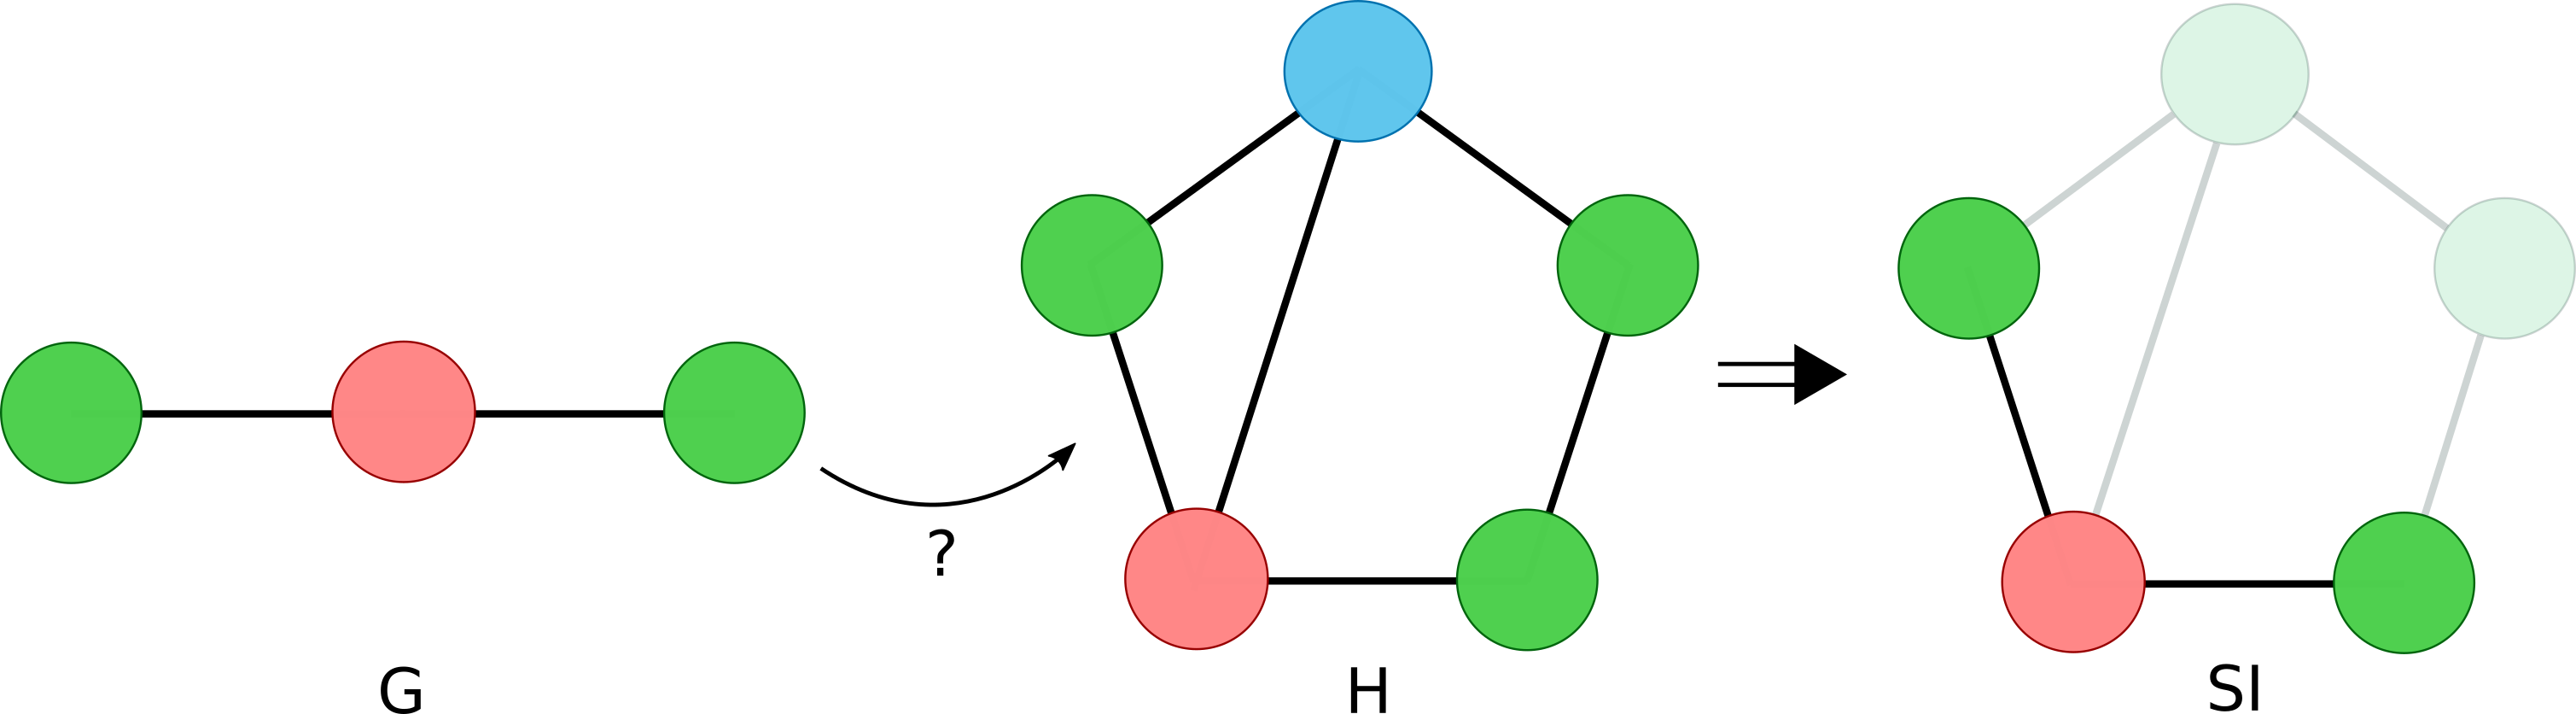
\includegraphics[width=450px]{Figures/s2m/MCS-SI/si.png}
    \caption{\label{SI_fig}SI obtenu à partir de la recherche du graphe G dans H.
    Sur cet exemple, il n'y a qu'une seule possibilité mais si nous avions cherché une chaîne comme Vert-Rouge-Bleu, nous aurions eu deux SI différents.}
  \end{center}
\end{figure}

\paragraph{}Définissions à son tour le problème SI.
Comme le nom l'indique, le problème SI est un problème de recherche d'un graphe dans une sous partie d'un autre.
C'est à dire que G est sous graphe de H lorsque tous les n\oe{}uds et toutes les arêtes de G sont retrouvées structurées de la même manière dans H (voir figure \ref{SI_fig}).
Tout comme le MCS, le problème du SI à été prouvé NP-Complet\cite{garey_computers_1979}.

\paragraph{}Pour notre problème, nous pouvons à nouveau effectuer une réduction vers le problème SI, puis résoudre ce problème par des algorithmes déjà publiés.
Nous souhaitons rechercher des monomères au sein de peptides, ce qui reviendrait à chercher plusieurs fois un petit graphe atomique monomérique dans un gros graphe atomique peptidique.

\paragraph{}Les méthodes de résolution actuelles sont toutes très similaires et dérivent d'une même technique de backtracking.
La plupart de ces méthodes sont des résolutions exactes.
Bien que NP-complet, ces algorithmes restent très praticables lorsqu'on ne recherche pas au sein de graphes répétitifs (qui sont constitués de multiples répétitions d'un même morceau).
Voyons ensemble quelques uns de ces algorithmes.


\subsubsection{L'algorithme de Ullman}

\begin{figure}[!ht]
  \begin{center}
    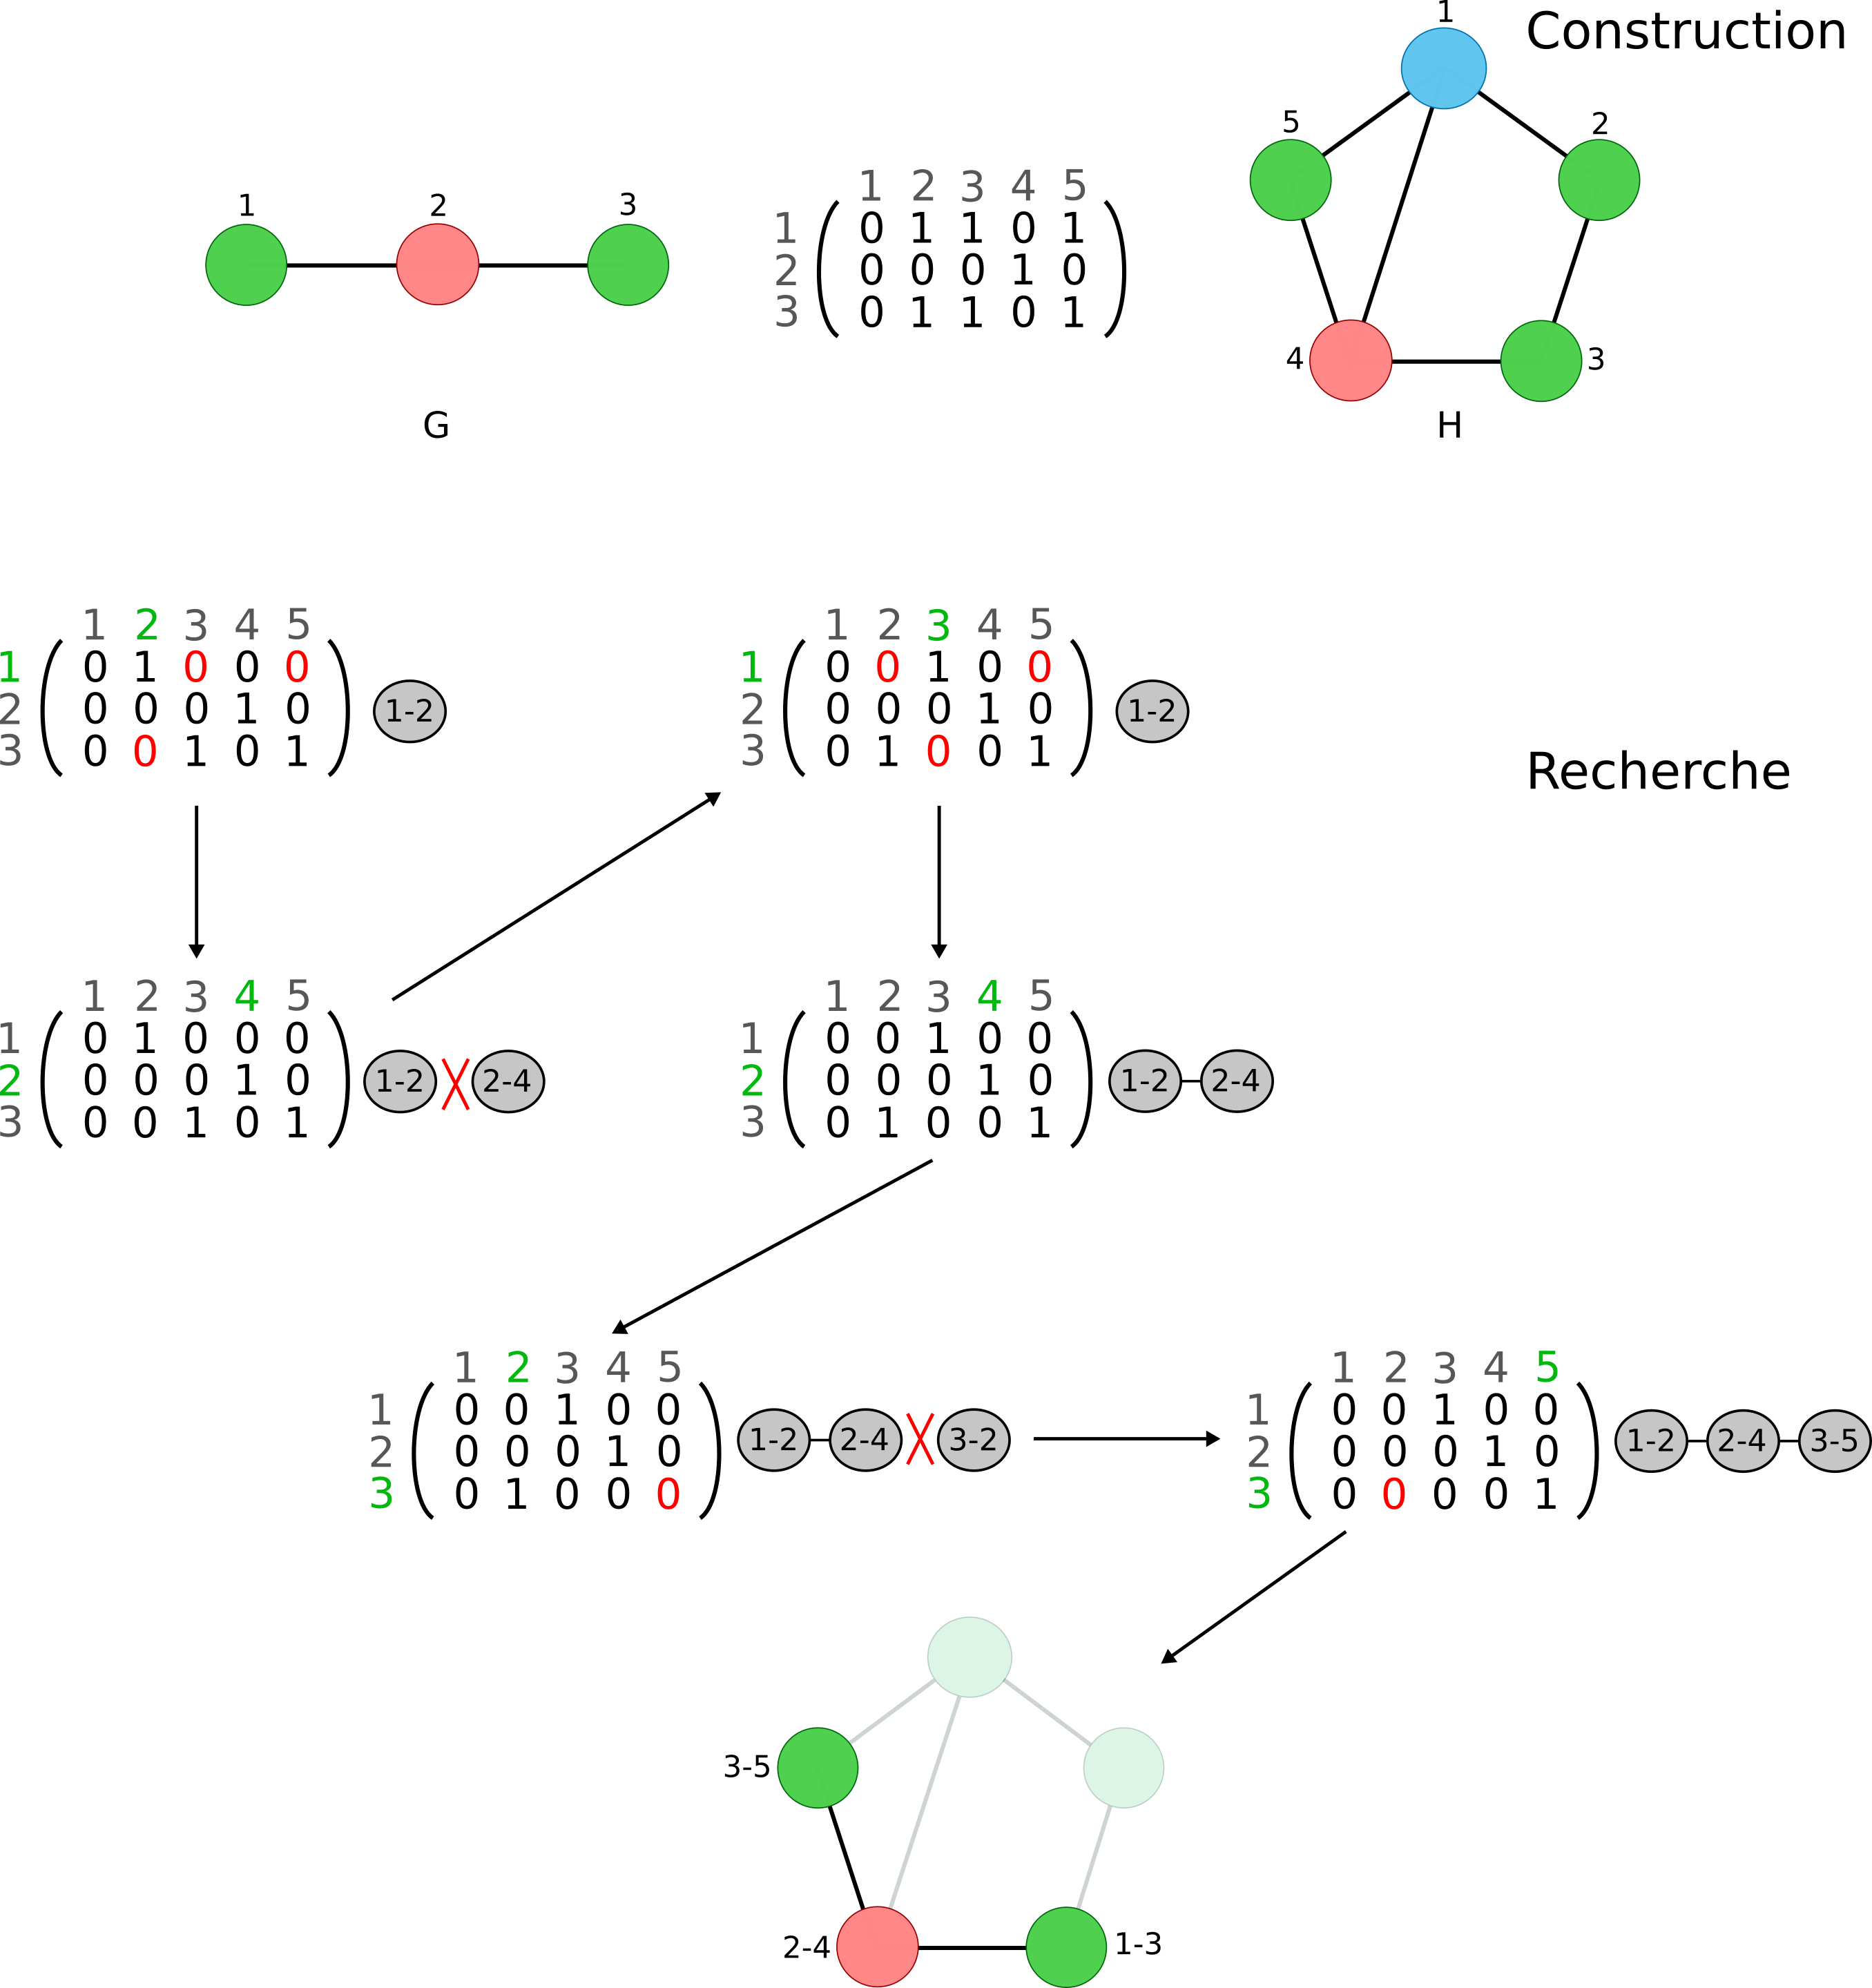
\includegraphics[width=450px]{Figures/s2m/MCS-SI/ullman.png}
    \caption{\label{ullman_fig}Recherche d'un isomorphisme de sous graphe par l'algorithme d'Ullman.
    Dans la partie construction, vous pouvez voir la matrice créée à partir des graphes G et H.
    Dans la partie recherche sont présentées les étapes successives de création d'un SI (voir texte pour détail).
    Si nous avions voulu obtenir tous les isomorphismes (et pas juste un seul), il aurait fallu continuer le backtracking jusqu'au bout.}
  \end{center}
\end{figure}

\paragraph{}L'algorithme de Ullman est l'un des premiers à avoir été proposé dans les années 70~\cite{ullmann_algorithm_1976}.
Certaines de ses variantes sont toujours utilisées dans certaines librairies telles que Openbabel~\cite{oboyle_open_2011}.
L'algorithme se base sur la matrice de compatibilité entre les graphes (voir figure \ref{ullman_fig}).
Une matrice de compatibilité est une matrice dont chaque ligne représente les n\oe{}uds de G et chaque colonne les n\oe{}uds de H.
Pour une case de la matrice donnée, on a $g$ le n\oe{}ud de G correspondant à la ligne et $h$ le n\oe{}ud de H correspondant à la colonne.
La case contient un 1 si $g$ et $h$ ont une étiquette compatible et que l'arrité de $h$ est suppérieure ou égale à l'arrité de $g$.
Pour obtenir un SI à partir de cette matrice, il faut retirer des 1 de la matrice jusqu'à en obtenir uns seul 1 par ligne.
A chaque étape, un n\oe{}ud de G est choisi pour continuer l'isomorphisme.
Ce n\oe{}ud correspond à une ligne.
Puis une colonne est choisie parmi celles dont la colonne contient un 1 sur la ligne précédemment choisie.
Le couple ligne/colonne nous donne le couple n\oe{}ud de G/n\oe{}ud de H a peut être ajouter à l'isomorphisme.
Avant cet ajout, il faut également vérifier que tous les voisins du n\oe{}ud de H correspondent bien aux voisins du n\oe{}ud de G (condition non respectée à l'étape 2 et 5 de la partie recherche du schéma).
Puisque nous ajoutons ce binôme à l'isomorphisme, il faut remplacer tous les 1 de la ligne et la colonne choisies par des 0 (excepté pour la case du binôme).
À ce moment, si au moins une ligne a été vidée de tous ses 1, c'est que l'isomorphisme n'est pas possible et il faut revenir à l'étape précédente.
Sinon, il suffit de continuer récursivement jusqu'à obtenir un unique 1 par ligne.
En choisissant bien les lignes et les colonnes par lesquelles l'algorithme commence, on arrive à obtenir des temps d'exécution très courts pour la recherche d'un SI.
Cependant, pour obtenir tous les SI, il faut parcourir tout l'arbre des possibles, ce qui ralentit l'algorithme.


\subsubsection{Les algorithmes de backtracking classique}

\paragraph{}Tout comme pour le MCS, le SI peut être résolu par un backtracking classique par association de n\oe{}uds deux à deux.
C'est la méthode majoritairement utilisée puisqu'elle fonctionne très bien en pratique.
Contrairement à l'algorithme d'Ullman qui nécessite d'effectuer des opérations sur des matrices potentiellement très grandes, la méthode par backtracking classique n'a pas besoin de grands espaces mémoire.
L'algorithme VF2~\cite{cordella_subgraph_2004} utilisent ce principe.
Les SI se forment par ajouts successifs de couples de n\oe{}uds compatibles avec retour en arrière s'il n'est plus possible d'avoir un couple.
Nous donnerons plus de détails sur cet algorithme en section \ref{VF2_p}.
Cet algorithme est utilisé dans les grandes librairies logicielles de chimie comme CDK~\cite{steinbeck_chemistry_2003}.


\subsubsection{D'autres algorithmes de SI}

\paragraph{}Contrairement à la recherche de MCS, il n'existe pas beaucoup d'alternatives heuristiques pour ce problème.
Ceci peut s'expliquer par le fait que des algorithmes praticables existent pour trouver les SI.
De plus, les heuristiques de MCS permettent d'obtenir des résultats de SI en ajoutant des contraintes (Le SI étant un cas particulier du MCS).
Dans tous les cas, ces heuristiques de SI sont des dérivés de la technique par backtracking~\cite{kaijar_developing_2012}.
Ces algorithmes essaient en supplément d'éviter l'exploration de toutes les branches par de la sélection des plus ``prometteuses''.

\paragraph{}Il existe également de nombreux algorithmes pour des cas particuliers de SI.
Par exemple, il est possible de résoudre le problème en temps polynomial pour des arbres~\cite{shamir_faster_1997}, des graphes planaires~\cite{eppstein_subgraph_1995,dorn_planar_2009} ou des graphes de treewidth bornés~\cite{hajiaghayi_subgraph_2007}.
Dans tous les cas, il est possible de trouver au moins une molécule ne répondant pas à l'un de ces critères et c'est pour cela que nous ne les utiliserons pas.


\subsection{Choisir l'algorithme de recherche de monomères}

\paragraph{}Pour pouvoir rechercher les monomères nous devions choisir entre toutes les approches algorithmiques citées ci-dessus.
Premièrement, lorsque nous recherchons un monomère dans un peptide, nous souhaitons connaître tous les endroits où il peut apparaitre.
Nous ne souhaitons donc pas utiliser d'approches heuristiques.
Deuxièmement, le MCS ne paraît pas très pratique dans notre cas.
En effet, les NRP regorgent de monomères proches les uns des autres.
Il n'est donc pas facile, lorsque l'on obtient un résultat, de savoir si la molécule trouvée est la bonne ou si c'est le monomère voisin à un atome de distance qui a été détecté.
Enfin, en comparant les algorithmes de recherche exacte de solutions, ceux de résolution de SI sont plus adaptés et rapide en pratique.
C'est pourquoi nous avons choisi d'effectuer la recherche des monomères en utilisant l'algorithme le plus communément utilisé par la communauté : VF2.




\section{Construction algorithmique}

\subsection{Isomorphisme de sous graphe appliqué à la recherche de monomères}

\label{isomorphisme_p}

\paragraph{}La première partie Smiles2Monomers doit rechercher l'ensemble des monomères au sein d'un polymère cible.
Comme nous l'avons vu dans l'état de l'art, nous pouvons transformer ce problème en un problème de graphe appelé isomorphisme de sous graphe.
Dans cette partie, nous allons présenter en détail l'algorithme classique de recherche de SI nommé VF2 en l'étendant à des graphes étiquetés.
Puis nous montrerons en quoi les étiquettes des n\oe{}uds du graphes influencent le temps de calcul afin en déduire une méthode de recherche efficace.

\subsubsection{L'algorithme originel VF2}

\label{VF2_p}

\paragraph{}Comme nous l'avons déjà évoqué dans l'état de l'art de cette partie, l'algorithme VF2 permet d'effectuer des
isomorphismes de graphes ou de sous-graphes non étiquetés d'un graphe $G$ sur un graphe $H$.
Écrivons l'algorithme tel qu'il est décrit dans l'article d'origine :

\paragraph{}
  \begin{algorithm}[H]
    \caption{Algorithme VF2 pour graphes non étiquetés}
    \KwData{Un graphe $G(V,E)$ et un graphe $H(V',E')$ avec $|V| \leq |V'|$ et $s$ un état contenant les mappings déjà effectués
    entre les deux graphes}
    \KwResult{Un mapping entre les éléments de $V$ et une sous partie des éléments de $V'$ telle que $H$ soit un isomorphisme de
    sous graphe de $H$}
    
    \uIf {$s$ contient un mapping de tous les éléments de $V$} {
      \KwRet $Mapping(s)$\;
    } \uElse {
      \uIf {$Mapping(s)$ est vide} {
	$P \gets$ ensemble des $p(x,y)$ tq $x \in V$ et $y \in V'$ \;
      } \uElse {
	$P \gets$ ensemble des $p(x,y)$ tq $x \in V$, $y \in V'$ et $\exists p(a,b) \in Mapping(s)$ tq $a$ et $x$ soient voisins dans
	$G$ et $b$, $y$ voisins dans $H$ \;
      }
      
      \For {$p \in P$} {
	$s' \gets p \cup s$\;
	\If {$VF2(G, H, s') != \emptyset$} {\KwRet $Mapping(s')$\;}
      }
      
      \KwRet $\emptyset$ \;
    }
  \end{algorithm}

\begin{figure}[!ht]
  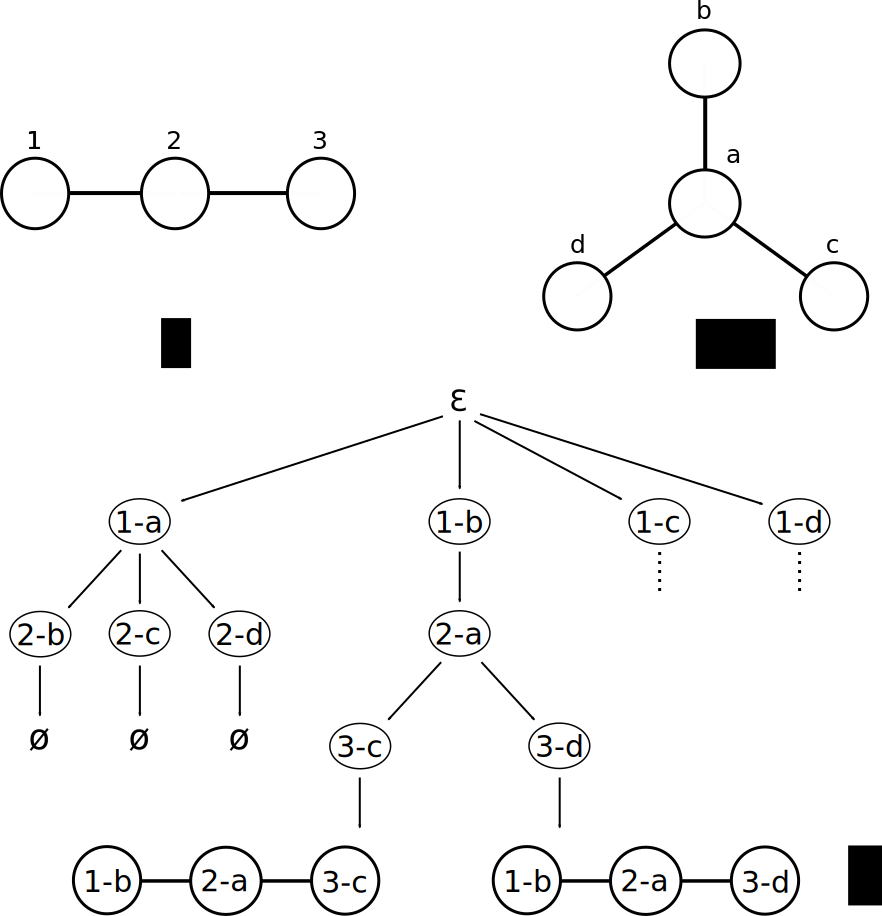
\includegraphics[width=200px]{Figures/s2m/recherche/VF2.pdf}
  \caption{\label{vf2}Représentation sous forme d'arbre d'une recherche de d'isomorphisme de sous graphe par l'algorithme VF2}
\end{figure}

\paragraph{}Expliquons cet algorithme en utilisant le schéma \ref{vf2}.
A la première étape, nous nous trouvons avec un ensemble vide de n\oe{}uds pairés de $G$ et $H$.
Nous générons donc toutes les possibilités d'assemblage entre tous les n\oe{}uds des deux graphes (Il est à noter que l'algorithme
est décrit de cette façon dans l'article mais qu'il n'est nécessaire de générer que les couples à partir d'un seul n\oe{}ud de $G$
et de l'ensemble des n\oe{}uds de $H$.)
Une fois ces assemblages créés, nous les parcourons tous en appelant récursivement la fonction.
Dans l'exemple, le premier appel récursif est effectué après avoir assemblé '1' à 'a'.
Cette voie est sans issue car quel que soit l'assemblage entre '2' et un n\oe{}ud de $H$, plus aucun couple de voisins ne pourra être
généré.
En effet, pour générer l'ensemble $P$, il est nécessaire de regarder tous les voisins de 'b' alors que le n\oe{}ud ne possède plus
de voisins hors de $s$.
Une fois toutes les tentatives échouées, l'algorithme remonte dans l'arbre et change l'association '1'-'a' pour l'association
'1'-'b'.
Récursivement l'algorithme conclut à un isomorphisme {(1,b);(2,a);(3,c)}.

\paragraph{}En l'état, l'algorithme VF2 ne reconnaît qu'un seul et unique isomorphisme.
On peut modifier simplement l'algorithme afin de récupérer tous les isomorphismes en ne retournant pas une fois que l'un d'eux est
trouvé mais en l'enregistrant dans un ensemble puis en continuant l'exploration de l'arbre jusqu'au bout.
Vu que tout l'arbre est exploré à chaque recherche, l'algorithme est exponentiel.
Pour être plus précis il est en $O(n^m)$, donc non calculable dans les pires des cas ($n$ taille de G et $m$ de H).

\begin{figure}[!ht]
  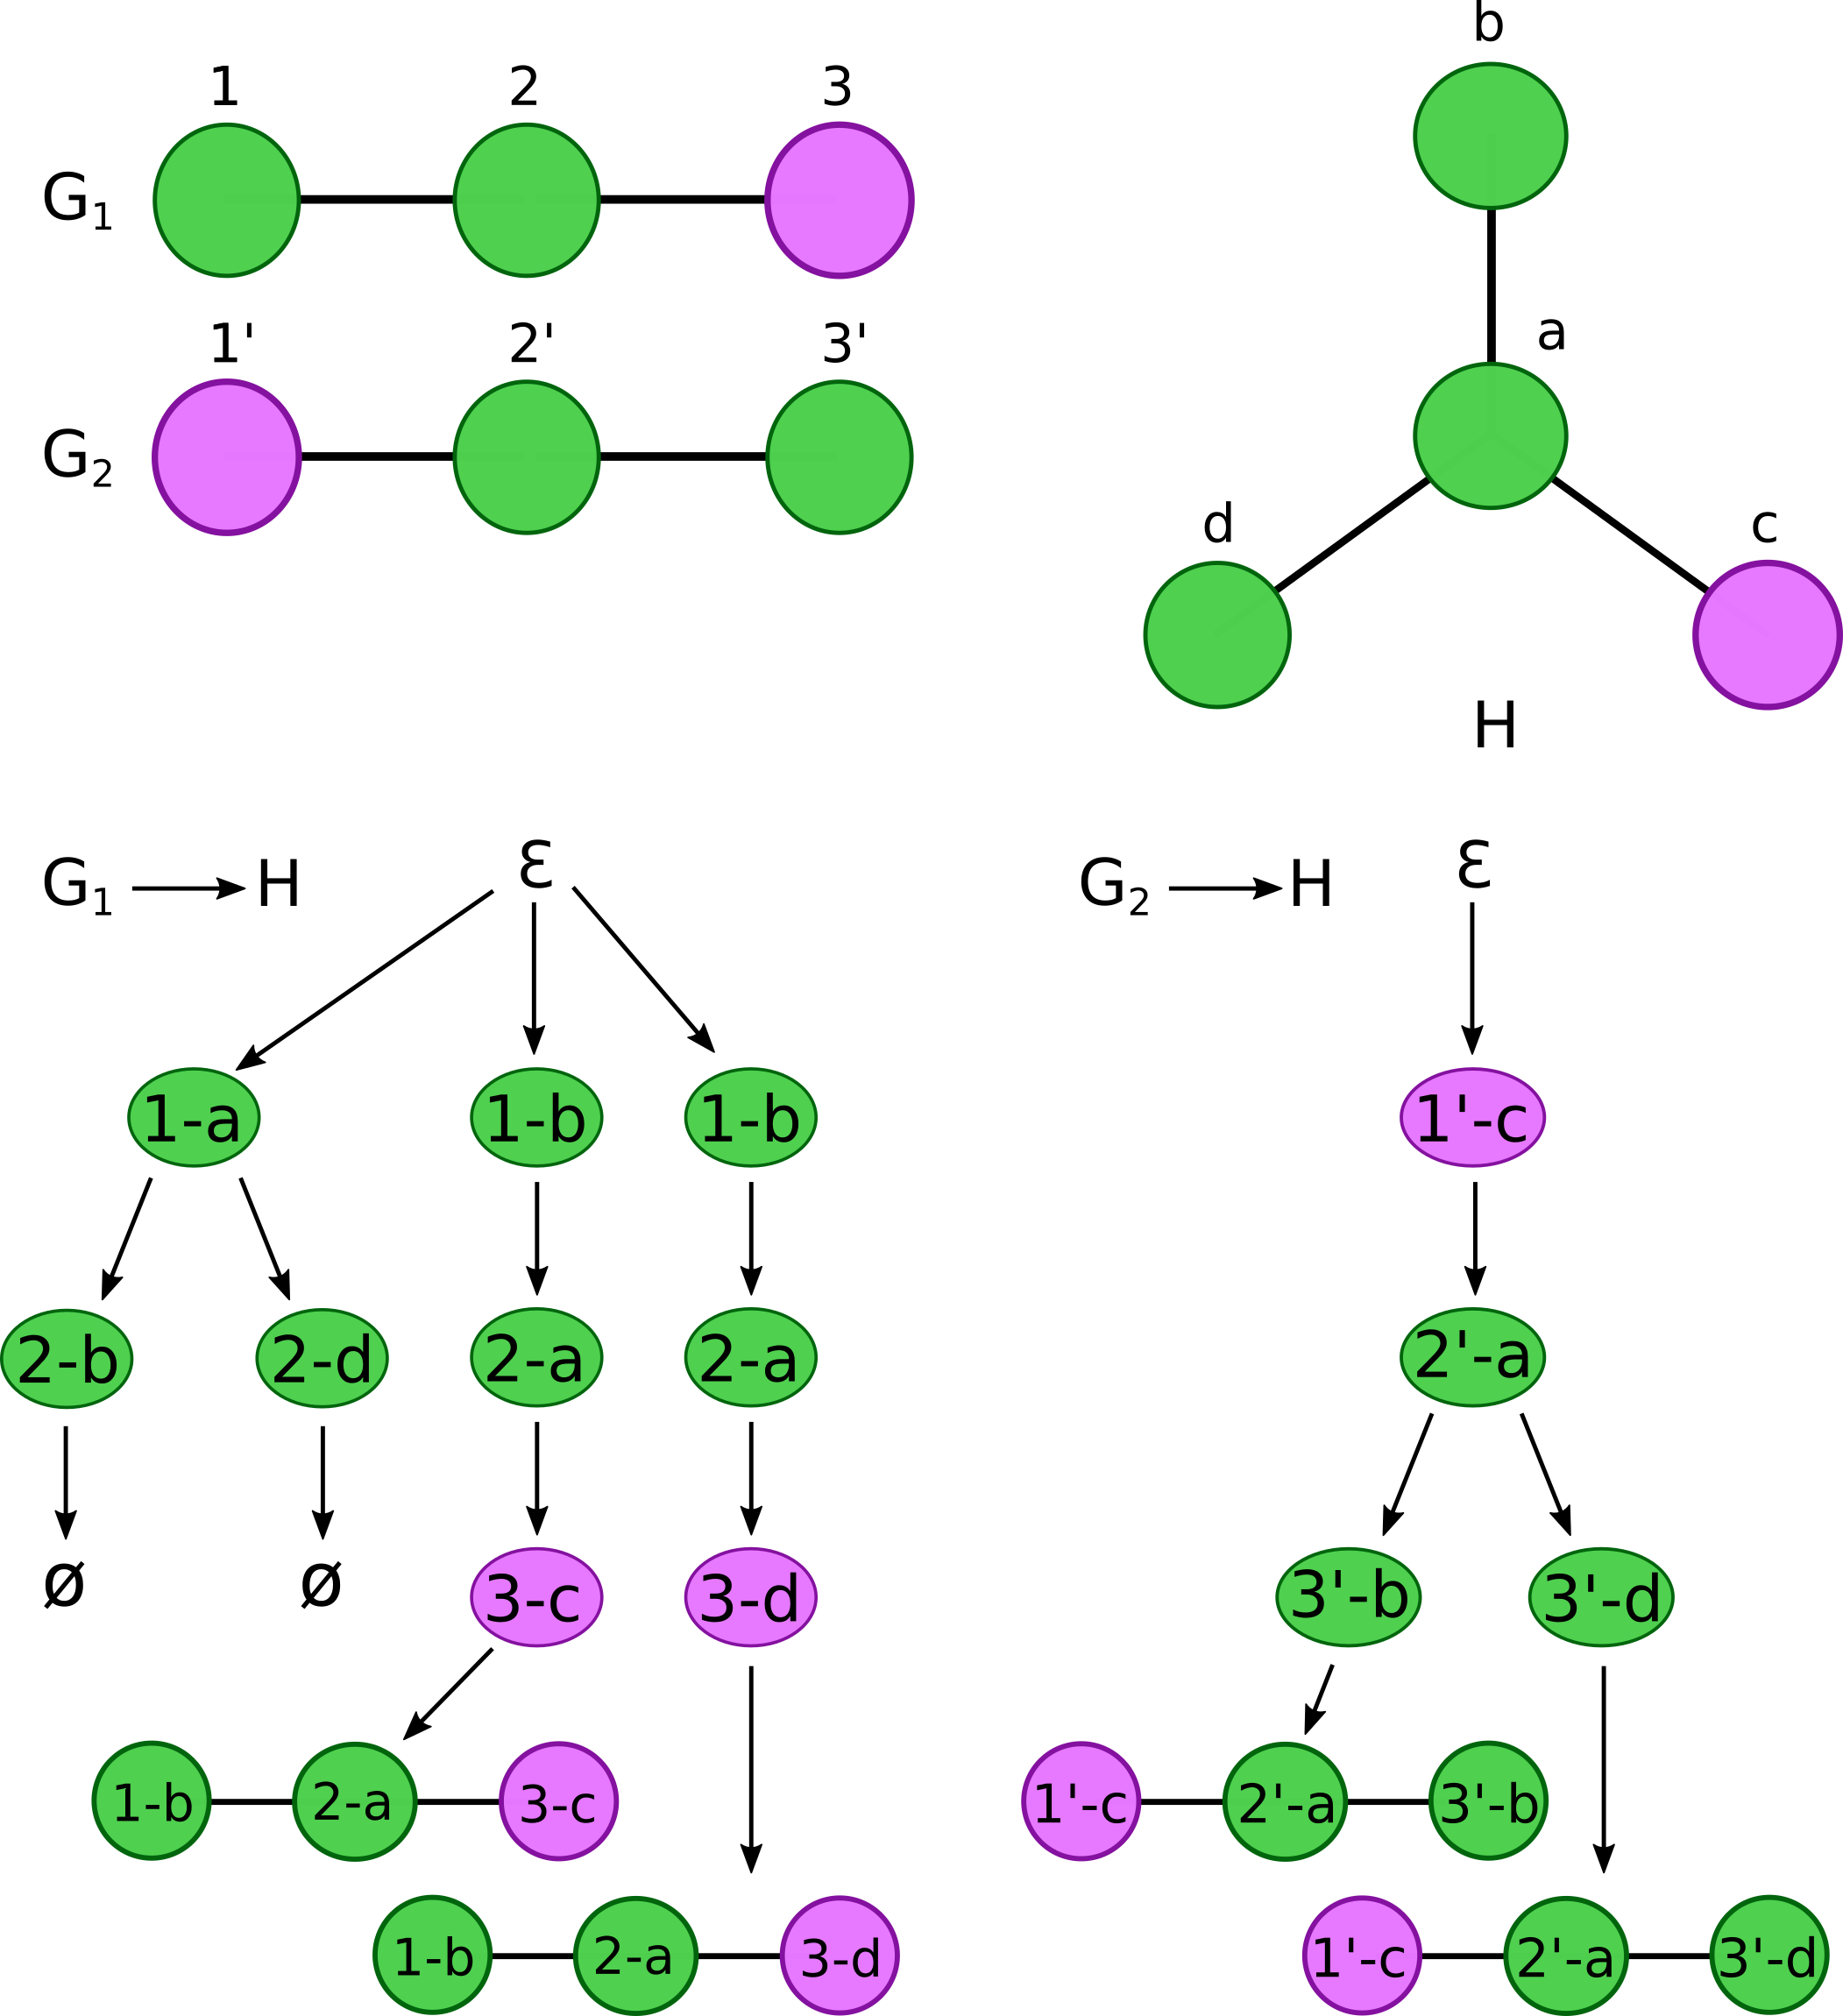
\includegraphics[width=200px]{Figures/s2m/recherche/VF2_labels.pdf}
  \caption{\label{vf2_labels}Représentation sous forme d'arbre de recherches pour l'algorithme VF2 appliqué aux graphes étiquetés}
\end{figure}

\paragraph{}Intéressons nous maintenant aux graphes étiquetés.
On peut modifier l'algorithme VF2 pour qu'il ne prenne en compte que les paires de n\oe{}uds possédant la même étiquette.
Prenons à nouveau notre exemple précédent en étiquetant avec A et B les n\oe{}uds.
Sur la figure \ref{vf2_labels}, on peut voir la recherche d'un graphe $G$ composé de 2 n\oe{}uds A et un n\oe{}ud B au sein d'un graphe $H$
composé d'un branchement supplémentaire contenant un n\oe{}ud B.
Sur ce graphique nous avons représenté deux cas de recherche selon l'ordre dans lequel nous prenons $G$.
Nous pouvons remarquer que dans les deux cas, la taille de l'arbre est bien plus faible que pour un graphe non étiqueté.
Les étiquettes des n\oe{}uds font office de filtres de recherche et accélèrent fortement la recherche.
On voit également que la recherche est d'autant plus rapide que l'on choisit prioritairement les n\oe{}uds avec des étiquettes de faible
fréquence.

Là où l'algorithme général VF2 était en $O(n^m)$, la complexité est ici réduite dans le pire des cas à $O(k^n)$ où $k$ est le
comptage du nombre de n\oe{}uds de l'étiquette la moins filtrante.
La taille de l'arbre de recherche est diminuée par la sélectivité des étiquettes de n\oe{}uds.
Pour optimiser la recherche, nous devons donc étudier la façon dont nous représentons les molécules afin d'avoir une sélectivité
la plus grande possible.

\subsubsection{Sélectivité d'un n\oe{}ud}

\paragraph{}Premièrement, attachons nous à la représentation la plus basique possible d'un graphe chimique (atome=n\oe{}ud,
liaison=arête). Dans cette représentation, nous pouvons considérer chaque étiquette comme étant le nom de l'atome du n\oe{}ud (Voir
figure \ref{representations}, première partie). Évidemment, les hydrogènes sont les atomes les plus représentés et ne filtrent
pas les recherches par eux-mêmes. Cependant, ils sont un bon moyen de donner des précisions sur l'atome auquel ils sont liés.
Ainsi, trouver un $CH_{3}$ ou un $CH$ donne une information différente sur la topologie.
En prenant en compte la remarque précédente, nous avons créé une seconde représentation qui compresse les hydrogènes à l'intérieur
des n\oe{}uds représentant les atomes plus lourds.
Ainsi, plusieurs étiquettes différentes peuvent
désormais être créés pour un même atome et ce, en fonction de ses compagnons hydrogènes (Voir figure \ref{representations},
seconde partie). Par exemple $NH_2$, $NH$, $N$ sont les
trois étiquettes variants depuis l'ancienne étiquette unique $N$ qui était accompagnée de voisins hydrogènes. Les étiquettes sont plus nombreuses et leur fréquence à la fois moins élevée et plus homogène, ce qui les rend plus sélectives.

\begin{figure}
  \includegraphics[width=300px]{Figures/s2m/representations/all_tmp.pdf}
  \caption{\label{representations}Manque fréquences et titres dans l'image}
\end{figure}

\paragraph{}Globalement, plus le nombre d'étiquettes est élevé et leurs fréquences sont homogènes, et moins l'algorithme VF2 aura de
difficultés à effectuer un isomorphisme. En effet, la lenteur qui peut venir de cet algorithme est due au nombreux chemins qu'il
peut prendre lors de l'exploration.

\paragraph{}Cherchons encore à augmenter la sélectivité des étiquettes en augmentant leur nombre. A partir d'un graphe $G$, il est
possible de représenter ses relations d'adjacence au sein d'un second graphe $L$. Pour cela, deux n\oe{}uds voisins de $G$ sont
représentés dans $L$ comme un seul n\oe{}ud. Chaque ancienne arrête devient un n\oe{}ud et chaque ancien n\oe{}ud devient une multitude
d'arêtes (une clique entre tous les nouveaux n\oe{}uds représentant les anciennes arête de cet ancien n\oe{}ud). Nous étendons le 
raisonnement pour les étiquettes en disant que l'étiquette d'un n\oe{}ud du nouveau graphe est la composition des étiquettes des anciens
n\oe{}uds ainsi que de l'arité entre ces deux n\oe{}uds (Dans notre cas, les étiquettes sont mis dans l'ordre lexicographique pour ne pas
avoir deux étiquettes possibles à partir des étiquettes d'origine)(Voir figure \ref{representations},
troisième partie). Un tel type de graphe est appelé line graph~\cite{orlin_line-digraphs_1978}. L'un des
gros avantages de cette représentation est d'inclure directement dans les étiquettes des n\oe{}uds ce qui touche à l'arité entre n\oe{}uds.
La fonction
de recherche n'aura donc plus du tout à s'attarder sur les liens mais uniquement sur les n\oe{}uds. De plus, transformer les graphes
de cette manière nous permet de répondre à la volonté d'augmentation du nombre d'étiquettes. Là où la représentation précédente
pouvait avoir $n$ étiquettes différentes, celle-ci pourra générer plus de $n^2$ ($3n^2$ si on compte tous les type de liaison entre
n\oe{}uds).

\paragraph{}Le raisonnement des line graphe peut être étendu récursivement. On peut ainsi créer des line-graph de line-graph.
Cependant cela pose plusieurs problèmes de répéter cette opération dans notre cas. Certains graphes vont diminuer de taille
jusqu'à disparaître complètement (ce qui est peu pratique pour la comparaison) alors que d'autres vont grossir de plus en plus
et ajouter de plus en plus de phases de comparaison d'étiquettes et d'étapes dans l'algorithme VF2. Pour ces raisons, nous avons
choisi de n'effectuer qu'une seule étape de line-graph.

\begin{figure}
  \includegraphics[width=200px]{Figures/s2m/recherche/matching.pdf}
  \caption{\label{label_matching}Exemple de fonctionnement de la fonction de matching d'étiquettes}
\end{figure}

\subsubsection{Indexation des monomères}

\label{index_p}

\paragraph{}Connaissant la sélectivité pour une étiquette, nous cherchons désormais à savoir l'ordre dans lequel il faut rechercher
un motif afin de minimiser le temps de recherche.
Nous appellerons \textbf{motif} le graphe compressé que nous allons vouloir retrouver dans un plus
grand graphe. Définissons également une \textbf{chaîne} comme étant un motif plus un ordre dans lequel parcourir ce motif. Ainsi,
on peut avoir plusieurs chaînes représentant le même motif mais avec des ordres de parcours différents. Ce que nous appellerons
indexation sera donc la phase de création d'une chaîne pour représenter chaque motif d'intérêt en essayant de minimiser le temps
que prendra la recherche de cette chaîne. Pour la recherche de monomères dans
des peptides non ribosomiques, la phase d'indexation revient donc à choisir, pour chaque monomère, l'ordre dans lequel nous allons
rechercher les n\oe{}uds du graphe le représentant. Ainsi, on peut voir que quelque soit la chaîne représentant le graphe, le même
motif sera toujours recherché. La seule différence sera la rapidité d'exécution de la recherche. Les deux sections suivantes
s'attarderont à la recherche de chaînes performantes (\textit{ie} les plus rapide) lors la recherche d'un motif.


\subsubsection{Indexation gloutonne}

\begin{figure}
  \includegraphics[width=300px]{Figures/s2m/indexation/chaine_fail.pdf}
  \caption{\label{chaine_fail}Deux exemple de chaîne pour un motif simple}
\end{figure}

\paragraph{}Une bonne chaîne est donc une chaîne rapide ; mais à quoi ressemble une telle chaîne ? Déterminons quel(s) critère(s)
simple(s) nous permettent de supposer qu'une chaîne est bonne. Avec ce ou ces critères, nous pourrons ensuite déterminer un
moyen d'ordonner les n\oe{}uds de manière gloutonne. Partons de l'exemple présenté sur la figure \ref{chaine_fail}. A gauche est
dessiné un motif simple suivi de deux chaînes pouvant le représenter (lecture de l'ordre des chaînes de gauche à droite). Pour
la première chaîne, en partant du motif ne contenant qu'un A, on obtiendra 3 isomorphismes. En étendant ces chaînes à deux A
voisins, on conserve toujours trois isomorphismes puis deux en ajoutant B et enfin un seul avec le dernier A. Au total, on aura
étendu 9 isomorphismes durant la recherche. En regardant maintenant la seconde chaîne, on se rend compte que le nombre de ces
isomorphismes intermédiaires est bien plus faible grâce à la sélectivité du B recherché en tout premier (5 isomorphismes
intermédiaires sont étendus). La différence décisive entre les deux chaînes est donc le moment où le n\oe{}ud avec une étiquette sélective
est recherché. Si le n\oe{}ud B est recherché dès le début, la solution est ``ancrée'' sur une base solide et ne risque pas de 
créer trop de solutions intermédiaires qui devront toutes être analysées pour passer à l'étape suivante. On peut dire qu'un n\oe{}ud
est plus sélectif qu'un autre à partir du moment où sa fréquence d'apparition dans les molécules étudiées est moins élevée.

\paragraph{Étiquettes fréquentes}

\begin{figure}
  \includegraphics[width=300px]{Figures/s2m/indexation/apprentissage.png}
  \caption{\label{apprentissage}En haut de l'image est représentée la base d'apprentissage puis en bas, le motif qui doit être
  indexé ainsi que les fréquences d'apparition de chacun de ses n\oe{}uds dans la base d'apprentissage}
\end{figure}

\paragraph{}Essayons d'estimer ces fréquences afin d'éviter les cas qui pourraient être critiques. Pour ce faire, nous pouvons
constituer un ensemble représentatif du type de molécules que nous allons chercher.
Dans notre cas, nous cherchons à étudier des peptides non ribosomiques. La base d'apprentissage
des fréquences sera donc constituée de NRP dont la composition atomique est déjà connue. Le raisonnement est extensible à
n'importe quel type de molécules et le fait d'avoir un jeu d'apprentissage non représentatif n'influencera pas le résultat mais
uniquement le temps de calcul. Une fois cette base créée, nous pouvons estimer les fréquences d'apparition de chacune des étiquettes
présents dans les monomères en effectuant une recherche exhaustive (Figure \ref{apprentissage}). L'algorithme glouton naïf qui
vient tout de suite en tête est de choisir un à un les n\oe{}uds que l'on souhaite ajouter au motif en choisissant toujours celui
avec l'étiquette la moins fréquente.

\paragraph{}
  \begin{algorithm}[H]
    \caption{Algorithme glouton de création de l'ordre des n\oe{}uds pour le parcours d'un graphe}
    \KwData{Un graphe $G(V,E)$}
    \KwResult{Une liste $N$ contenant tous les n\oe{}uds de V ordonnés pour la recherche}
    \SetKwFunction{recur}{recur}\SetKwFunction{algo}{trier}
    \SetKwProg{myalg}{fonction}{}{}
    \myalg{\algo{$G(V,E)$}}{
      \KwRet \recur{$G(V,E)$, \{\}}\;
    }
 
    \myalg{\recur{$G(V,E)$, $N$}}{
      \eIf {$|N| == |V|$}{
	\KwRet $N$\;
      } {
	Prendre tous les voisins des n\oe{}uds présents dans $N$ qui ne sont pas présent dans $N$\;
	Choisir le n\oe{}uds $n$ avec l'étiquette la moins fréquente\;
	Ajouter $n$ à la fin de $N$\;
	\KwRet \recur {$G(V,E)$, $N$}\;
      }
    }
  \end{algorithm}


\paragraph{}Il est nécessaire de préciser que la recherche des n\oe{}uds voisins peut être faite en maintenant
un ensemble des voisinages. L'algorithme glouton naïf est donc linéaire par rapport à la taille du graphe. À l'exécution, la
création de chaînes par cette méthode est instantanée ($\ll$ 0.1s). Toutefois, rien ne garantit la qualité des chaînes obtenues.
Prenons l'exemple de la figure \ref{apprentissage}. Sur cet exemple, le motif à indexer est a-b-d. Les comptages des différentes
étiquettes nécessaires sont également présents sur cette même figure. La chaîne qui sera générée commence forcément par le n\oe{}ud
étiqueté $a$ (fréquence la plus faible dans le jeu d'apprentissage) suivi de $b$ puis enfin $d$ (Le tout est résumé sur la figure
\ref{glouton}).

\begin{figure}
  \includegraphics[width=300px]{Figures/s2m/indexation/glouton.png}
  \caption{\label{glouton}En vert le chemin pris par l'algorithme glouton pour générer la chaîne du motif a-b-d}
\end{figure}

\subsubsection{Indexation Markovienne}

\label{index_markov}

\paragraph{}En utilisant la méthode gloutonne, nous obtenons rapidement les chaînes de tous les motifs que nous
souhaitons indexer. Cependant, dans certains cas, une chaîne générée de cette manière peut ne pas du tout être optimale.
Dès le tout début de la chaîne, il est possible que l'algorithme fasse des choix optimaux localement qui vont ensuite mener à un
enlisement global. Nous allons nous appuyer sur les figures \ref{apprentissage} et \ref{glouton} pour monter que même sur un si
petit exemple, l'algorithme glouton n'a pas choisi le meilleur chemin.

\paragraph{}Afin d'évaluer la qualité d'une chaîne, nous allons calculer son temps d'exécution sur notre base d'apprentissage.
Partons de la définition d'une chaîne : une chaîne est composée d'une succession de n\oe{}uds. Ces n\oe{}uds vont, lors de l'isomorphisme,
être recherchés dans l'ordre. Pour rechercher une chaîne de taille $n$ ($c_n$), il faut donc $n$ extensions successives. On
peut donc écrire que le temps de recherche d'une chaîne est le temps cumulé de recherche de ses extensions :

\begin{equation}
 T(c_n) = T(p_0 \rightarrow p_1 \rightarrow ... \rightarrow p_n) = \sum_{i=1}^n T(p_{i-1} \rightarrow cp_i)
\end{equation}

Où $T()$ est la fonction représentant le temps de recherche d'une chaîne, $p_i$ le un motif de taille $i$ et $p_{i-1} \rightarrow
p_i$ la dernière extension d'une chaîne $c_i$ représentée par le passage du motif $p_{i-1}$ au motif $p_i$. Il est à noter que
rechercher une chaîne de taille 1 revient à étendre un motif vide. C'est à dire qu'il est nécessaire de parcourir l'intégralité
des n\oe{}uds de la cible dans laquelle on recherche le motif et ce quel que soit le motif. Sur notre base d'apprentissage il faudra
donc tester tous les n\oe{}uds de tous les peptides d'apprentissage pour la première extension.

\begin{figure}
  \includegraphics[width=300px]{Figures/s2m/indexation/glouton.png}
  \caption{\label{arrite}Arité restante pour les différents n\oe{}uds d'un graphe chimique simple}
\end{figure}

\paragraph{}Lors d'une recherche d'une chaîne $c_{n-1}$, il est possible de trouver des isomorphismes sur la cible (potentiellement partiellement recouvrant).
Afin de calculer le temps de recherche de $c_n$ nous devons prendre en compte la quantité de sous isomorphismes précédemment trouvés.
Le calcul du temps de recherche de $c_n$ correspondra donc au temps de calcul de $C_{n-1}$ auquel on vient ajouter le temps de recherche de la dernière extension sur chacun des isomorphismes de taille $n-1$.
Il faut également tenir compte du nombre d'extensions qui vont être essayées.
Par exemple, si l'on cherche à étendre un isomorphisme précédent en suivant un lien qui est enraciné sur un $NH$, il ne reste qu'une liaison à explorer (le $N$ ayant déjà une liaison avec son $H$ et une liaison avec le reste du motif déjà recherché).
En reprenant la même logique pour un $C$, il resterait donc trois liaisons à suivre.
Nous appellerons cette quantité l'arrité restante.
On peut donc écrire :

\begin{equation}
 T(p_{n-1} \rightarrow p_n) = n_{p_{n-1}} \times a_{p_{n-1} \rightarrow p_n} \times t
\end{equation}

Où $n_{p_{n-1}}$ est le nombre d'isomorphismes trouvés pour le motif $p_{n-1}$, $a_{p_{n-1} \rightarrow p_n}$ est l'arité restante
de l'atome depuis lequel on étend le motif $p_{n-1}$ vers le motif $p_n$ et $t$ le temps nécessaire pour une comparaison de deux
étiquettes (ce temps peut être considéré constant)

\paragraph{}Combinons les deux équations précédentes, pour obtenir une formule globale :

\begin{equation}
 T(c_n) \propto^t N + \sum_{i=2}^n (n_{p_{i-1}} \times a_{p_{i-1} \rightarrow p_i})
\end{equation}

Où $N$ est le temps de calcul pour les chaines de taille 1.
Ce temps ne varie par car il est nécessaire de parcourir tout le graphe.

\begin{figure}
  \includegraphics[width=300px]{Figures/s2m/indexation/apprentissage_comptage.png}
  \caption{\label{app_compt}Base d'apprentissage accompagnée des comptages de tous les $n_{p_{n}}$}
\end{figure}

\paragraph{}En utilisant les comptages faits sur la base d'apprentissage (voir \ref{app_compt}) ainsi que le calcul de l'arité
restante de chaque n\oe{}ud à chaque étape, nous allons pouvoir estimer sur la base, un temps d'exécution de la recherche d'une
chaîne. Ce temps est un coût exact de le recherche sur la base d'apprentissage. En normalisant cette valeur par le nombre de
n\oe{}uds de la base, nous pouvons obtenir le coût de recherche par n\oe{}ud et ainsi pouvoir estimer le temps de calcul quelle que soit
la taille de la ou les molécules à analyser.

\begin{equation}
 T(c_n) \propto^t 1 + \sum_{i=2}^n ({n_{p_{i-1}} \over N} \times a_{p_{i-1} \rightarrow p_i})
\end{equation}

\paragraph{}Redéfinissons la notation ${n_{p_{i-1}} \over N}$ qui correspond à un taux de filtrage d'un motif de taille $i-1$.
Appelons ce taux $F_{i-1}$. Cette notation peut à son tour être transformée en
produit des filtrages de chaque extension d'une chaîne. Les valeurs des filtrages estimés s'obtiennent immédiatement à partir des
comptages dans la base d'apprentissage (Voir \ref{app_compt} pour un exemple). NB : Le taux de filtrage peut être supérieur à 1
car il est possible d'obtenir plus d'isomorphismes après une extension que avant.

\begin{equation}
 {n_{p_{i-1}} \over N} = F_{i-1} = \prod_{i=0}^{i-1} f_i
\end{equation}

\begin{equation}
 T(c_n) \propto^t 1 + \sum_{i=2}^n a_{p_{i-1} \rightarrow p_i} \prod_{j=0}^{i-1} f_j
\end{equation}

\paragraph{}Le temps de recherche optimal d'un motif est donc le temps de recherche de la chaîne qui minimise le coût. Donc :

\begin{equation}
 T(p_n) = \min T(c_n), \forall c_n
\end{equation}


\paragraph{}Appliquons maintenant cette formule de calcul du temps sur notre exemple pour trouver la meilleure chaîne possible par
rapport à la base d'apprentissage. Pour le motif de l'exemple, nous pouvons nommer les différentes chaînes possibles de $\alpha$
jusque $\delta$.

\[
\begin{array}{ccccccc}
 c         & = & p_1 & \rightarrow & p_2     & \rightarrow & p_3 \\
 c_\alpha  & = & a   & \rightarrow & a\!-\!b & \rightarrow & a\!-\!b\!-\!d \\
 c_\beta   & = & b   & \rightarrow & a\!-\!b & \rightarrow & a\!-\!b\!-\!d \\
 c_\gamma  & = & b   & \rightarrow & b\!-\!d & \rightarrow & a\!-\!b\!-\!d \\
 c_\delta  & = & d   & \rightarrow & b\!-\!d & \rightarrow & a\!-\!b\!-\!d \\
\end{array}
\]

On peut appliquer la formule sur chacune des chaînes possibles et trouver la chaîne optimale qui minimise la fonction de
coût. Développons l'exemple pour la chaîne $c_{\alpha}$.

\[
\arraycolsep=1.4pt\def\arraystretch{1.2}
\begin{array}{cccccccccccccc}
  c_\alpha    & =  & \epsilon &  \rightarrow &  \multicolumn{3}{c}{a} & \rightarrow & \multicolumn{3}{c}{a\!-\!b} &  \rightarrow & \multicolumn{1}{c}{a\!-\!b\!-\!d} &\\
  T(c_\alpha)   & =  & T( \epsilon &  \rightarrow &  a)  & + & T( a &  \rightarrow  & a\!-\!b) & + & T(a\!-\!b &  \rightarrow & a\!-\!b\!-\!d) &\\
                    & \propto_{N}  &  \multicolumn{3}{c}{1} &  + & \multicolumn{3}{c}{3 \times \frac{2}{18}} & + & \multicolumn{3}{c}{  (3-1)\times \frac{2}{18} \times \frac{3}{2}} &\\
                    & = &  \multicolumn{3}{c}{1} &  + & \multicolumn{3}{c}{\frac{1}{3}} & + & \multicolumn{3}{c}{\frac{1}{3}}   & \quad= \quad\frac{5}{3} \\

\end{array}
\]

\paragraph{}En appliquant cette formule sur toutes les chaînes, on peut se rendre compte que certains de nos calculs sont inutiles.
Prenons l'exemple des chaînes $c_{\alpha}$ et $c_{\beta}$. Le dernier calcul de la chaîne $c_{\beta}$ est inutile. Lors
du calcul des deux chaînes, on aurait pu se rendre compte que l'on pouvait déjà décider de quelle chaîne était la meilleure à
partir du résultat de la sous chaîne $a-b$. Ceci nous amène à transformer le calcul sous forme de programmation dynamique dont les
formules de récurrence sont les suivantes.


\begin{equation}
 T(\epsilon \rightarrow p_1) = 1
\end{equation}
\begin{equation}
 T(p_n) = \min^{p'_{n-1} \subset p_n} (T(p'_{n-1}) + T(p'_{n-1} \rightarrow p_n))
\end{equation}

Où la fonction de minimisation s'applique sur l'ensemble des $p'_{n-1}$ et $p'_{n-1}$ est un motif connexe de taille $n-1$ inclus
dans $p_n$. Pour la recherche de motif dans l'exemple, on obtient le chemin $c_{\delta}$ minimisant le coût. On peut voir le
détail de la recherche de ce motif sur la figure \ref{markov}.

\begin{figure}
  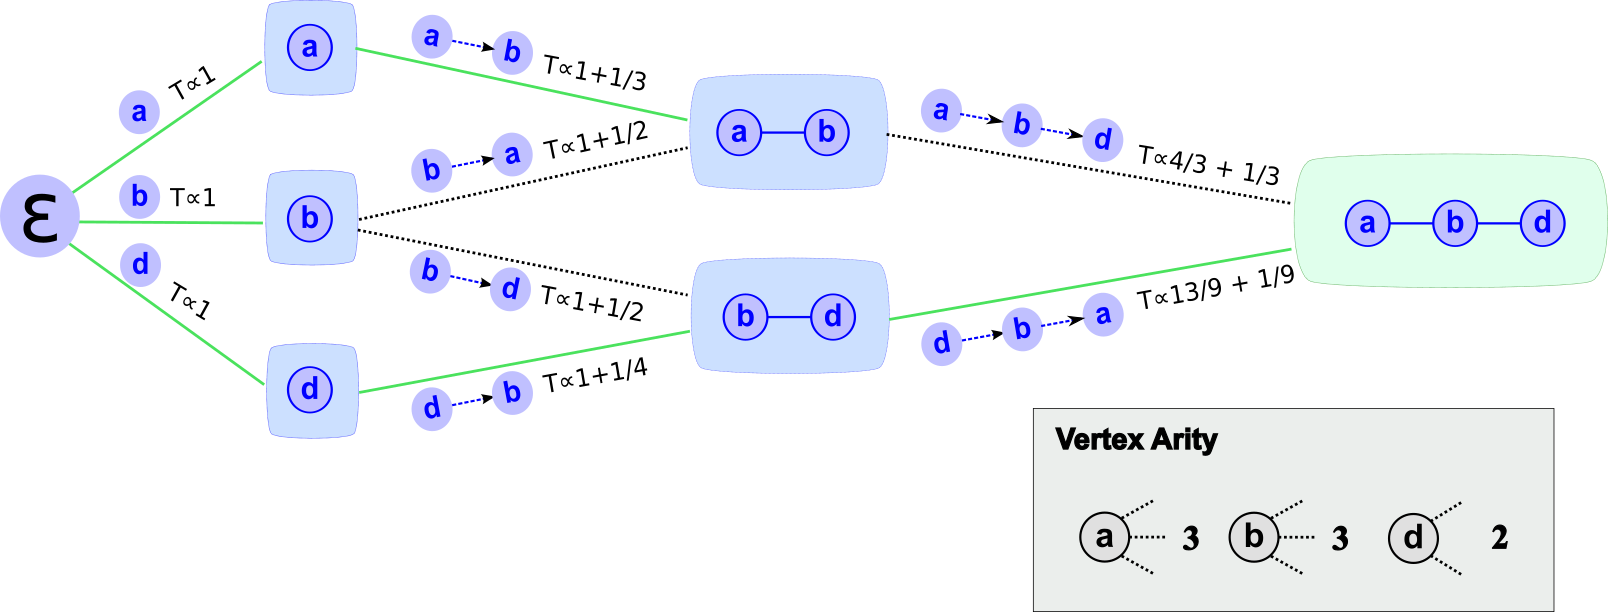
\includegraphics[width=300px]{Figures/s2m/indexation/markov.png}
  \caption{\label{markov}En vert, le chemin pris par l'algorithme markovien pour générer la chaîne du motif a-b-d}
\end{figure}

\paragraph{}Cette méthode exacte nous permet de garantir la qualité de nos chaînes sur la base d'apprentissage mais cela se paye en temps de calcul.
En effet, même par programmation dynamique le temps de pré-calcul des chaînes est très élevé si les motifs sont composés de nombreux branchements et d'une grande diversité de n\oe{}uds.
Calculons la complexité en considérant que chaque étiquette est unique.

Une chaîne (au sens ligne et pas chaîne comme défini ici) représente le motif le plus simple. Pour une chaîne de n\oe{}uds de taille 
$n$, on peut trouver un motif de taille $n$ puis deux de taille $n-1$ puis 3 de taille $n-2$, ... Pour calculer le coût du motif
de taille $n$, il nous faut calculer récursivement tous les motifs de taille inférieure. Dans le meilleur des cas la programmation
dynamique sera donc de complexité de l'ordre de $n^2$.

Le pire motif qui peut être défini est une clique. Dans le cas d'une clique de taille $n$, pour calculer le coût du motif, il faudra
calculer $n-1$ parmi $n$ valeurs puis $n-2$ parmi $n$, ... Dans ce cas, la complexité sera de l'ordre de $2^n$.

La redondance des étiquettes permet quant à elle de couper certaines branches lors de l'indexation et ainsi de diminuer un peu
la complexité. Cependant, l'ordre de grandeur n'en est pas modifié.

\begin{equation}
 Cplx_{chaine} = n + n-1 + ... + 2 + 1 = \sum_{i=1}^n i = {{n (n+1)} \over 2} = O(n^2)
\end{equation}
\begin{equation}
 Cplx_{clique} = {n \choose n} + {n \choose n-1} + ... + {n \choose 2} + {n \choose 1} = \sum_{k=1}^n {n \choose k} = O(2^n)
\end{equation}


\subsubsection{Indexation hybride}

\paragraph{}Dans un exemple précédent (TODO : ref), nous avons montré que le début d'une chaîne est très critique pour le temps
de recherche de celle-ci. L'idée est donc de générer la chaîne par un mélange des deux techniques précédentes. Les débuts de la 
chaîne seront recherchés en exact jusqu'à une taille $k$ définie à l'avance, puis le reste des extensions se feront en
utilisant l'algorithme glouton. Cette découpe des chaînes en deux parties garantit une recherche très rapide d'un
motif sur la base d'apprentissage tout en limitant fortement le temps de pré-calcul nécessaire pour la construction de l'index.



\subsection{Des monomères aux résidus}


\subsubsection{Résidus}

\paragraph{}L'algorithme et les indexes présentés dans la section précédente permettent de retrouver rapidement toutes les
occurrences d'un motif au sein d'une molécule cible. Jusqu'à présent nous avons laissé supposé que dans notre cas
nous recherchions des monomères dans des peptides. Ceci n'est en fait pas applicable directement. En effet, on ne retrouve jamais
un monomère en entier au sein d'un polymère. Lorsque les monomères sont liés ensemble pour former le polymère, chacun perd une
partie de ses atomes dans ces liaisons. Nous appellerons les molécules incluses des résidus (les monomères sans leurs atomes de
liaison).

\paragraph{}Prenons l'exemple de la Cystéine pour bien comprendre (Voir figure \ref{cys_ex}).
La cystéine est présente dans 47 peptides de la base de données
NORINE. Dans certains peptides comme ACV, la cystéine est incluse en effectuant deux liaisons peptidiques avec ses voisins. D'un
côté elle perd les atomes $OH$ de son groupement $COOH$ pour aller se lier à un groupe $NH_2$ qui perd un de ses $H$. Le tout
libère un $H_2O$ pendant la réaction. De l'autre côté elle perd un $H$ de son groupement $NH_2$ pour effectuer la même opération
inversée. Au total la cystéine présente dans ce peptide a donc perdu trois atomes sur deux sites distincts. Dans d'autre cas
comme dans la malformin A1, la cystéine effectue une troisième liaison au niveau de son atome de soufre en perdant un atome 
d'hydrogène pour se lier avec un autre atome de soufre et ainsi réaliser un pont disulfure. Sur ce simple exemple on remarque que
non seulement le monomère n'est jamais inclus en entier mais en plus, il peut être inclus dans un polymère de plusieurs manières
différentes. Il est donc nécessaire de connaître les différents résidus possibles pour chaque monomère afin de pouvoir les
rechercher en utilisant l'algorithme de recherche exact décrit précédemment.

\begin{figure}
  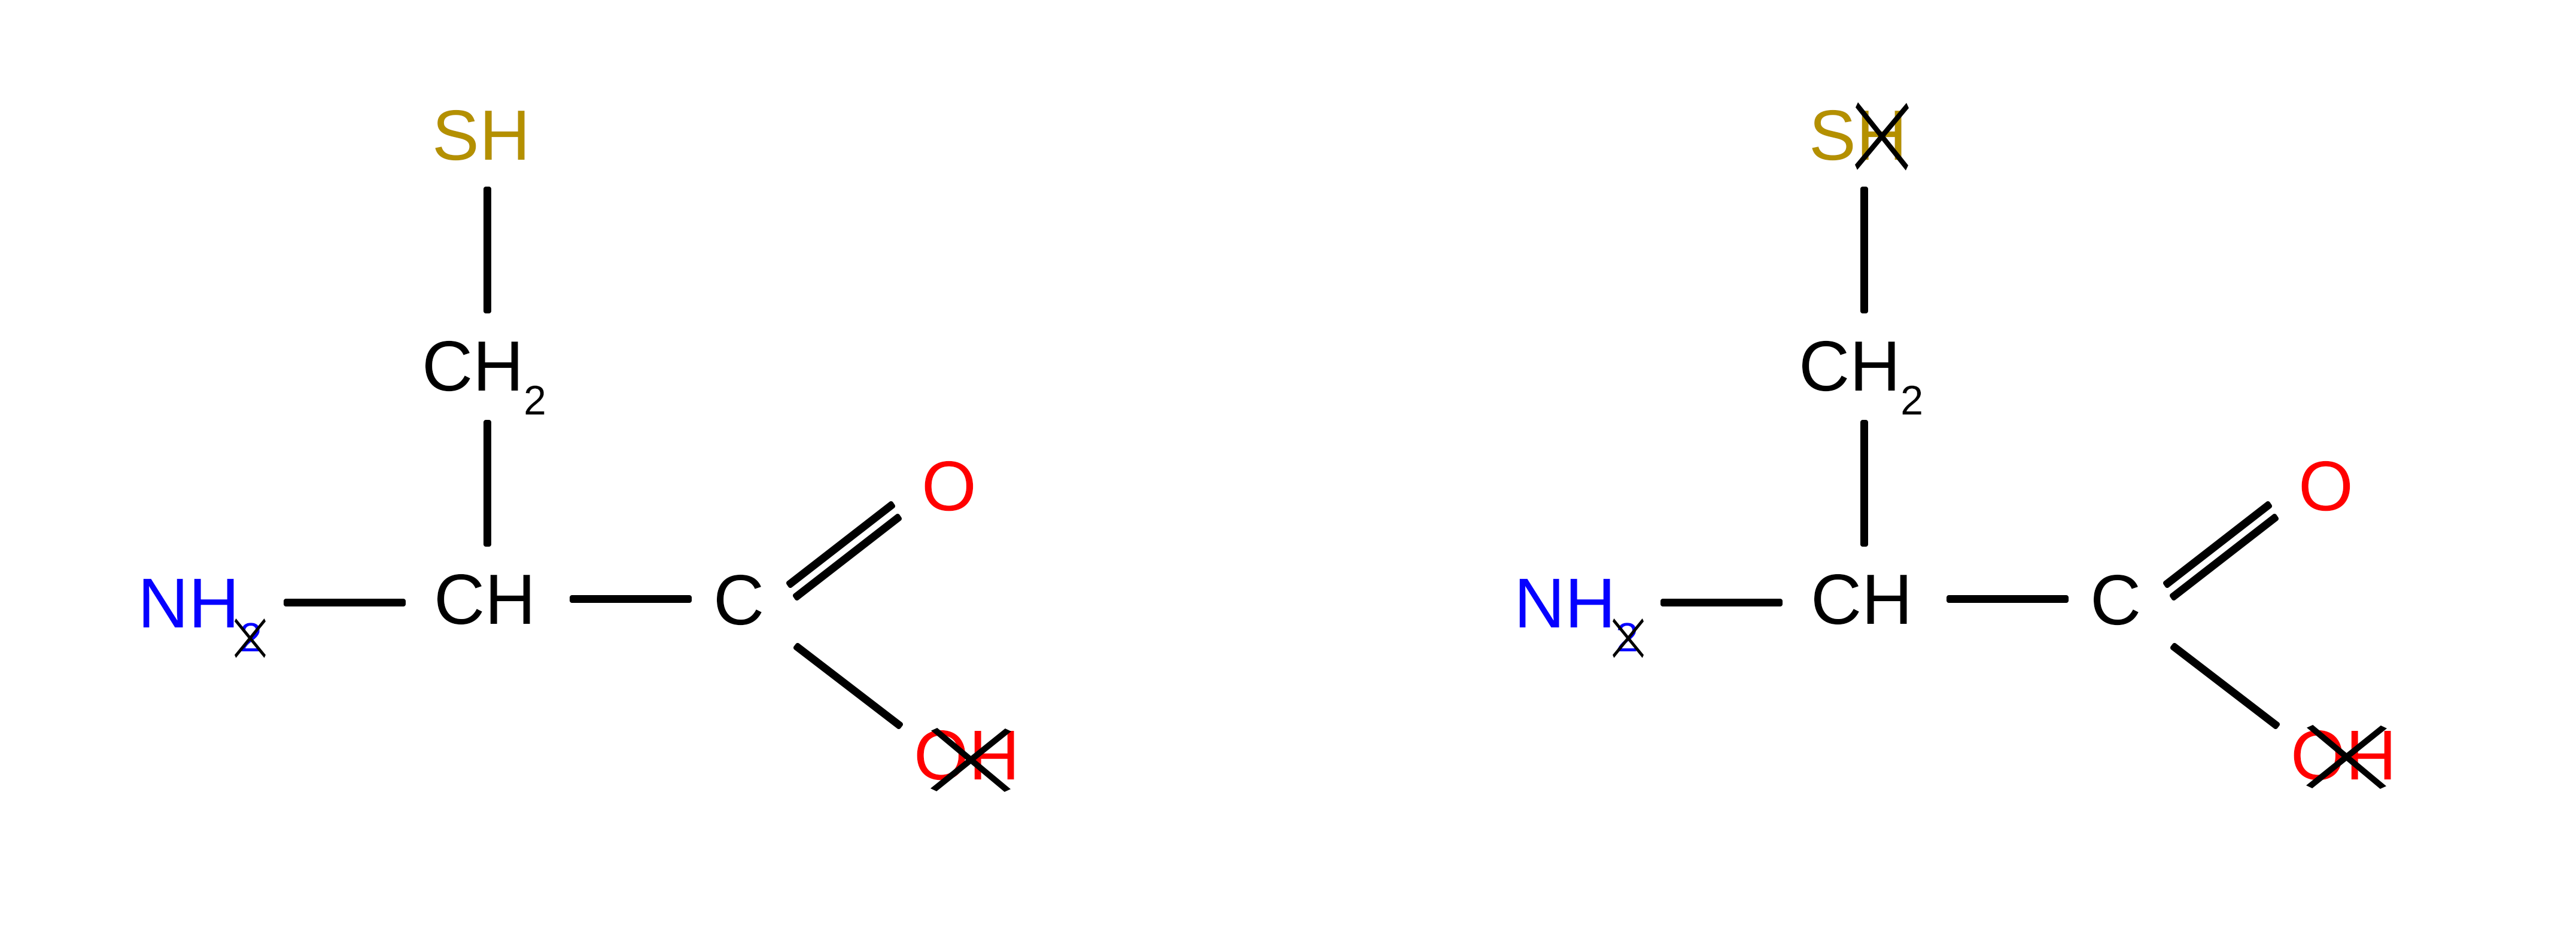
\includegraphics[width=300px]{Figures/s2m/residues/cys_exemple.pdf}
  \caption{\label{cys_ex}Deux résidus différents présents dans deux peptides différents tout deux obtenus à partir de la Cystéine}
\end{figure}


\subsubsection{Familles de résidus}

\paragraph{}Différents résidus d'un même monomère peuvent être créés selon les contextes. Pour connaître les différents résidus
possibles pour chaque monomère nous devons donc connaître les règles qui régissent les liaisons. Par exemple pour la liaison
peptidique précédemment citée, nous pouvons déduire deux règles. Si un $COOH$ est détecté alors le monomère peut potentiellement
perdre son $OH$. De la même manière pour la seconde moitié de la liaison on peut perdre un $H$ pour un $NH_2$ détecté. En
regardant précisément les liaisons qui apparaissent pour un type de polymère, nous pouvons créer une liste de règles de perte
d'atomes. En appliquant ses règles récursivement sur un monomère, nous pouvons générer tous ses résidus candidats. Notons que
certaines règles comme celles du pont disulfure décrite précédemment, ne s'applique qu'en présence d'une autre liaison. Il n'est
donc jamais nécessaire de générer le résidu qui contient uniquement cette liaison. Ici nous n'aurons donc jamais de résidus
uniquement constituée d'une liaison sulfure. Il est
à noter que moins une règle sera précise et plus le nombre de résidus générés sera important. Imaginons une règle qui nous dirait
dans un cadre de chimie organique que pour tout carbone étant lié à au moins un hydrogène, l'atome d'hydrogène peut être perdu
pour former une liaison. Si $n$ est le nombre d'atomes de carbone dans la molécule ($n$ représente une grande proportion d'atomes
dans une molécule organique), alors on peut générer un nombre de résidus de l'ordre de $n^2$.

\begin{figure}
  \begin{center}
    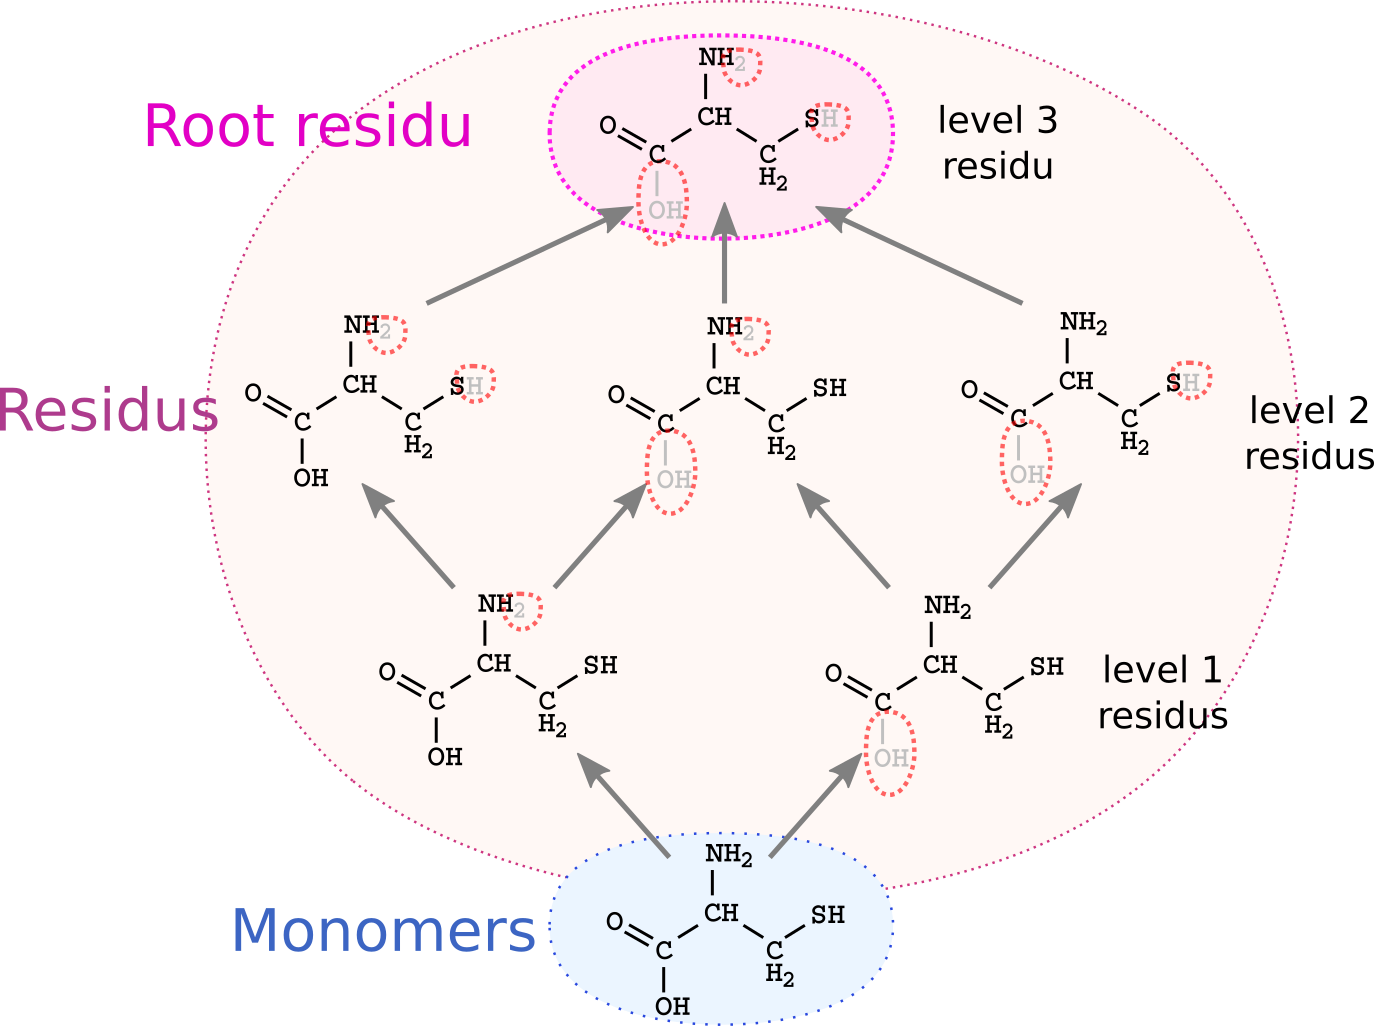
\includegraphics[width=400px]{Figures/s2m/residues/cystein_family.png}
    \caption{\label{sulfure}Représentation de la famille des résidus de la cystéine}
  \end{center}
\end{figure}

\paragraph{}Comme présenté dans la figure \ref{sulfure}, les différents résidus générés peuvent être représentés sous la forme
d'un Graphe Orienté Acyclique (GOA). Le monomère de base ainsi que chacun des résidus est un n\oe{}ud du graphe et chaque arc est un
lien de parenté entre n\oe{}uds. Un arc sera par exemple créé entre un résidu auquel on a appliqué une seule règle et le monomère.
Nous appellerons \textbf{famille} cette représentation des résidus sous forme de GOA.

\paragraph{}Le n\oe{}ud le plus éloigné du monomère sera le n\oe{}ud
qui aura subit le plus de modification. Nous appellerons le résidu de ce n\oe{}ud le \textbf{résidu racine}. Ce résidu à un intérêt
tout particulier pour la recherche du monomère. En effet, si le résidu racine n'est pas trouvé alors qu'il est celui
qui possède le moins d'atomes dans la famille, cela veut dire qu'aucun membre de la famille ne pourra être trouvé. On peut même
aller plus loin en étendant le raisonnement à tous les résidus. Si un résidu de niveau $n$ n'est pas trouvé alors il est inutile
de rechercher ses résidus parents de niveau $n-1$. Il est également vrai de dire qu'il est inutile de chercher un résidu parent de
niveau $n-1$ si tout ses enfants de niveau $n$ n'ont pas été trouvés.

\paragraph{}En connaissant la structure familiale des résidus ainsi qu'un ordre naturel de recherche pour passer d'un résidu à
l'autre, nous pouvons déduire une structure globale de recherche. Découle donc de cette structure familiale un ordre de recherche
naturel depuis le résidu racine jusqu'aux résidus de niveau 1 (Inutile de rechercher le monomère car il n'étant jamais inclus tel
quel). De plus, il n'est jamais nécessaire de
recalculer complètement un isomorphisme une fois que la racine trouvée. Pour passer d'un résidu $r$ à l'un de ses parents $p$ il
suffit de rechercher à étendre l'isomorphisme de $r$ avec les atomes que nous avions considérés perdus pour passer de $p$ à $r$
lors de la construction de la famille. De plus, le fait de ne pas tout recalculer à chaque étape nous autorise à ne calculer
l'index que pour les résidus racine. Le reste des résidus n'est indexé que sur les extensions a effectuer depuis leurs enfants.
L'algorithme qui décrit la recherche d'une famille est donc le suivant :

\paragraph{}
\begin{algorithm}[H]
  \caption{Algorithme de recherche des résidus d'une famille}
  \KwData{Un graphe $G(V, E)$ représentant le polymère cible et une famille $F_m$ de résidus pour le monomère $m$. Le résidu $r_r$
  étant le résidu racine de la famille.}
  \KwResult{Un ensemble de tuples constitués d'un résidu et d'un ensemble de position. Ces tuples représentent chacun un
  isomorphisme du résidu avec une sous partie du polymère.}
  Soit $S$ un ensemble de tuples solution initialement vide\;
  $S \gets subgraphIsomorphism (G, r_r)$\;
  
  \If {$S$ est vide} {
    \KwRet $S$\;
  }
  
  Soit $P$ un ensemble de résidus à procésser initialisé avec les parents de $r_r$\;
  \While {$P$ n'est pas vide} {
    $r \gets supprimeUnElement(P)$\;
    $Tmp \gets subgraphIsomorphism (G, r)$\;
    
    \If {$Tmp$ n'est pas vide} {
      Ajouter $Tmp$ dans $S$\;
      \For{$p \subset parents(r)$}{
	\If {Tous les enfants de $p$ ont été trouvés} {
	  Ajouter $p$ dans $P$\;
	}
      }
    }
  }
  
  \KwRet $S$;
\end{algorithm}




\subsection{Pavage de monomères}

\subsubsection{Pavage : définition}

\paragraph{}La méthode de recherche des isomorphismes de sous graphe présentée précédemment, trouve toutes les occurrences de chacun des monomères dans un peptide cible.

Puisque nous connaissons les atomes contenus dans chacun des isomorphismes découverts, nous pouvons également connaître chacun des
isomorphismes découvert par atome.
L'étape de pavage consiste à choisir un sous ensemble des isomorphismes trouvés, de manière à maximiser les atomes couverts par ces
isomorphismes en ayant pour chaque atome au plus un seul isomorphisme présent dans ce sous ensemble.

Faisons une analogie avec un puzzle. La phase d'isomorphisme créée de nombreuses pièces de puzzle.
Une reconstruction complète du puzzle n'est pas forcément faisable uniquement à partir de ces pièces.
De plus, parmi celles dont nous disposons, certaines se chevauchent.
La phase de pavage consiste à choisir parmi les pièces, celles que l'on souhaite garder en maximisant le remplissage de notre puzzle et sans avoir de pièces chevauchantes (figure \ref{puzzle}).

\begin{figure}
  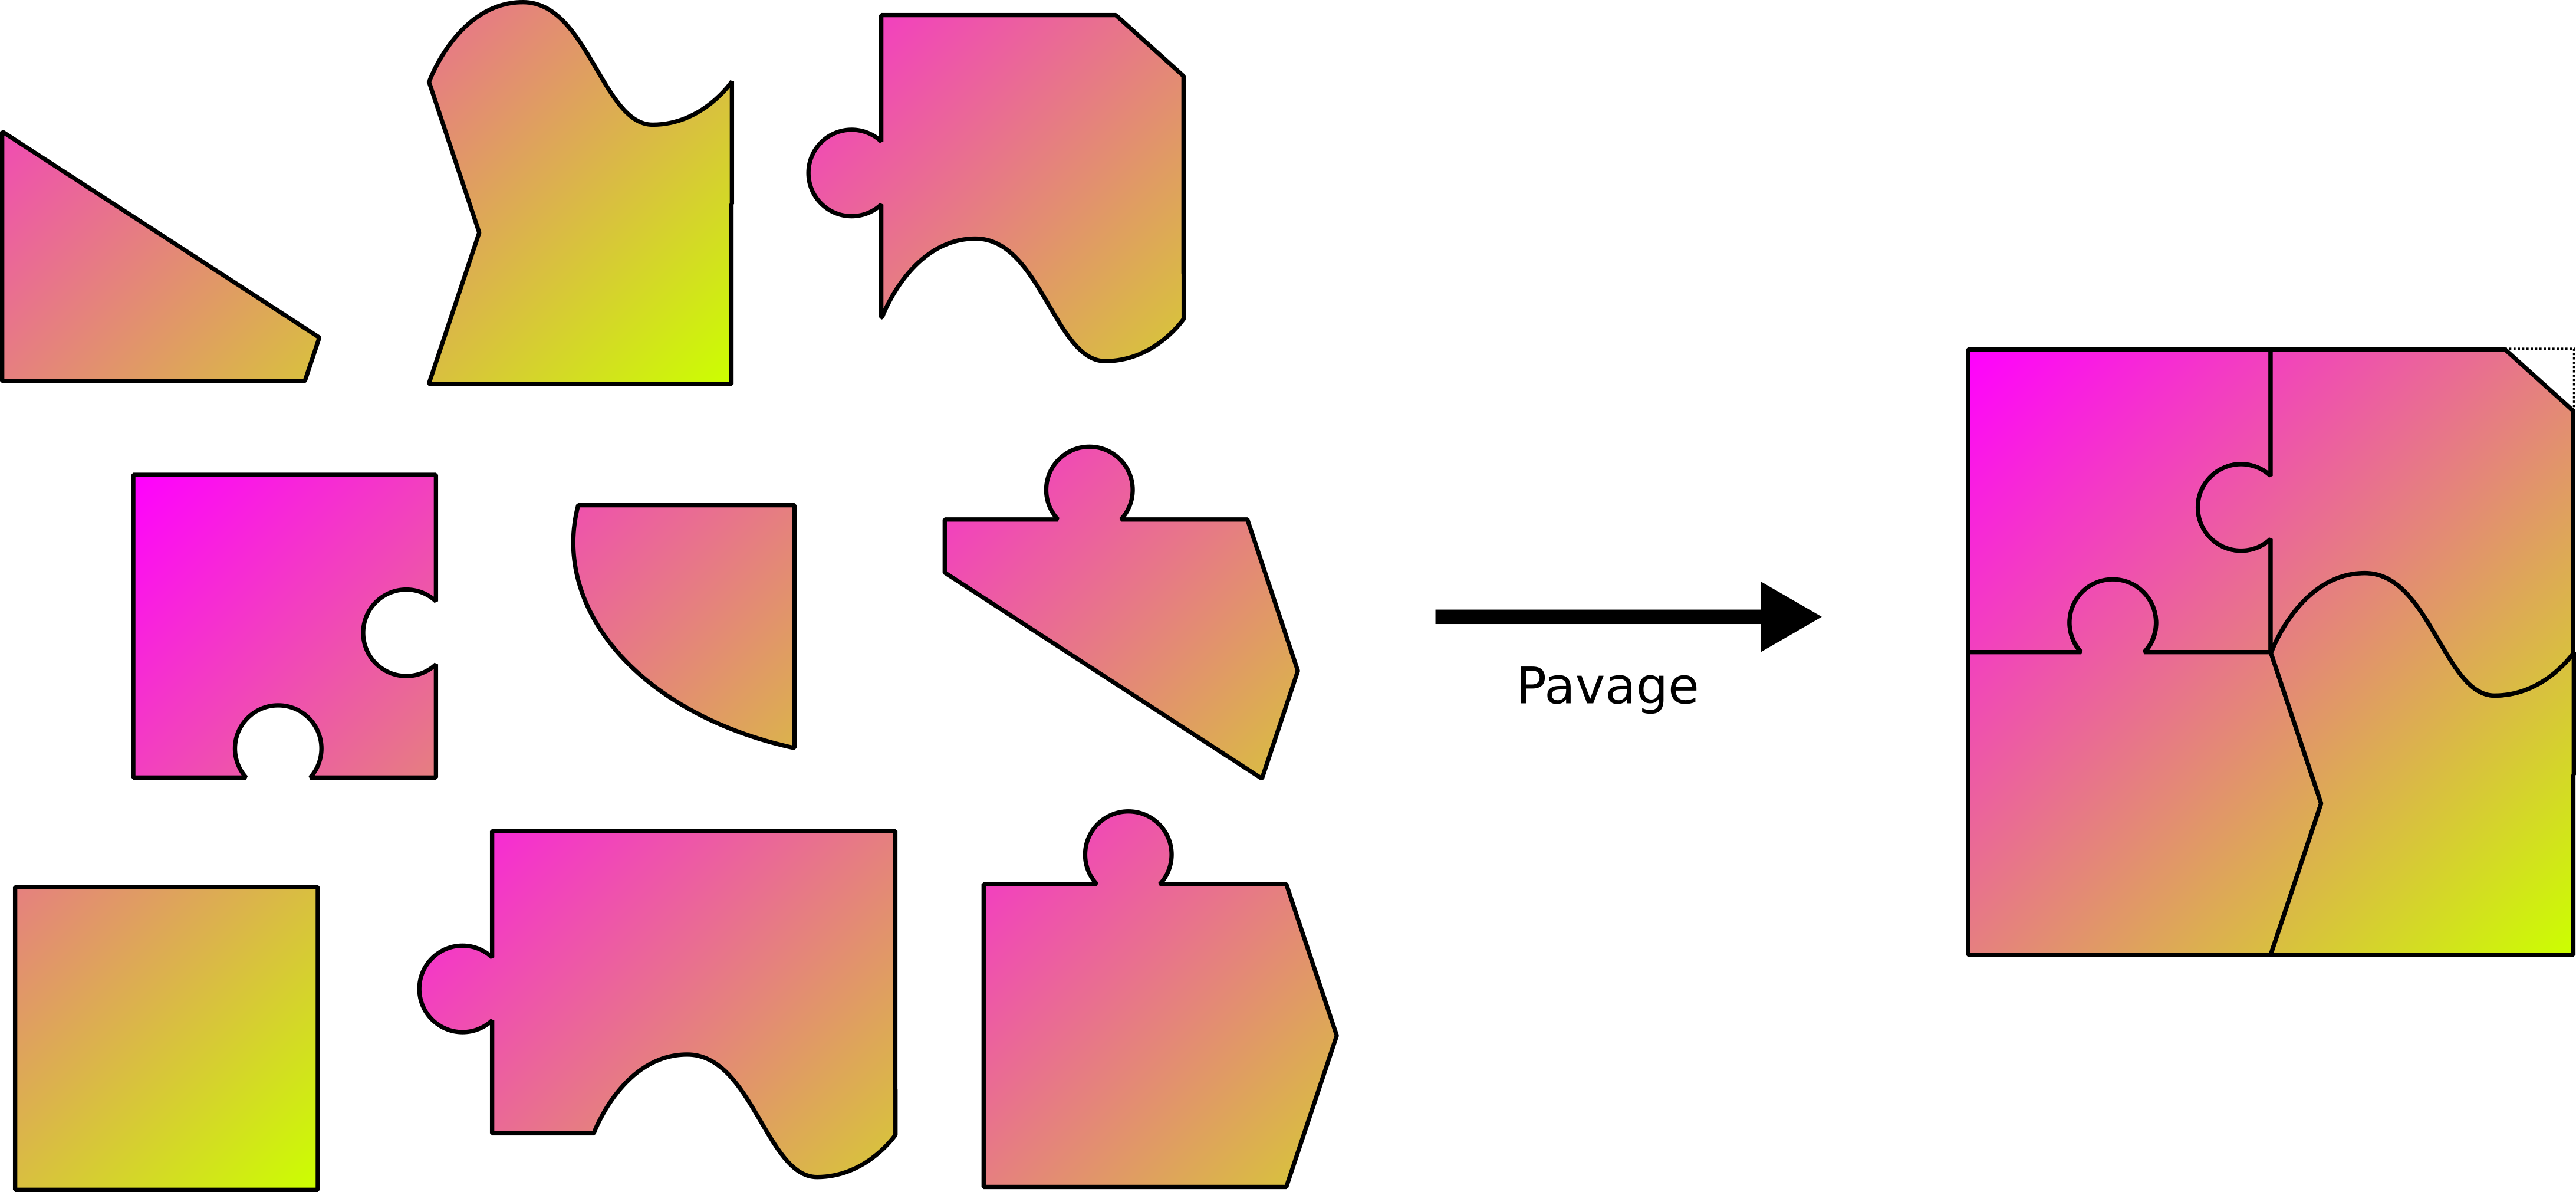
\includegraphics[width=300px]{Figures/s2m/pavage/puzzle.pdf}
  \caption{\label{puzzle}Un pavage est une recherche des meilleures pièces permettant de construire le puzzle des monomères}
\end{figure}

\paragraph{}Dans l'idéal, toutes les pièces nécessaire à la reconstruction du puzzle complet sont présentes dans l'ensemble des
pièces trouvées. Dans le cas contraire, on ne peut pas reconstruire complètement le peptide à partir des résidus trouvés. 
Dans ce cas, notre
but sera alors de trouver un assemblage le plus complet possible. Si beaucoup de résidus ont été trouvés lors de la première phase
il est également possible que nous ne trouvions pas qu'une seule solution de reconstruction. Nous n'aurons alors aucun moyen
purement algorithmique de choisir quelle est la meilleure façon de découper ces peptides.

\begin{figure}
  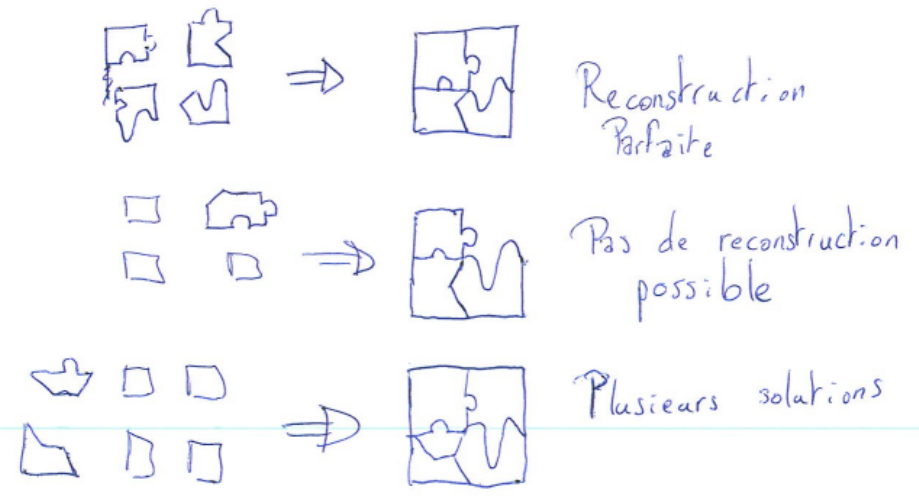
\includegraphics[width=300px]{Figures/s2m/pavage/reconstructions.png}
  \caption{\label{reconstruction}Les différents types de reconstruction que l'on peut obtenir par le pavage}
\end{figure}


\subsubsection{Preuve de NP-Complétude}

\paragraph{}En 2015 j'ai eu la chance de participer, avec mes amis Thomas Nachtergale et Alexandre Temperville, à la finale du concours d'algorithmique ``Google Hashcode''.
La veille de l'épreuve finale, un petit problème test nous a été proposé.
Le but était de découper une pizza (matrice), composée de cases de jambon (H dans la matrice) et de cases de sauce (T dans la matrice), en parts dites ``royales'', en minimisant le gâchis de pizza (morceaux ne contenant pas de parts).
Les part royales sont des parts rectangulaires contenant au minimum 3 cases de jambon et représentant une surface maximale de 12 cases.

\paragraph{TODO : schéma pizzas}

\paragraph{}Ce problème a été prouvé NP-Complet sur le forum stackexchange~\cite{de_biasi_complexity_2015} suite à la question d'un participant.
La preuve a été faite par réduction du problème ``Monotone cubic planar 1-3 SAT''.
Prouvons que le problème ``Pavage'' est également NP-Complet en utilisant une réduction du problème ``Pizza''.

\paragraph{}Premièrement, il est très facile de montrer par certificat que pavage est NP.
Le certificat contient l'ensemble des résidus pavés.
Leur nombre est borné par le nombre de résidus issus de l'isomorphisme.
Le certificat est donc de taille proportionnelle au problème.
Deuxièmement, le validateur de certificat doit vérifier qu'aucun résidu ne se chevauche.
Pour cela, il est possible de vérifier les chevauchements pour toutes les paires de résidus du certificat.
La vérification du certificat peut être faite de manière quadratique, ce qui permet de dire que le problème est NP.

\paragraph{}Prouvons ensuite que nous pouvons résoudre le problème Pizza en utilisant le problème Pavage.
Nous avons besoin de définir 3 notions pour notre codage :
\begin{itemize}
	\item Les atomes du peptide : Les atomes du peptide représenteront les cases de la matrice pizza.
	\item Les liens entre atomes : Les liens représentent les voisinage de deux cases.
Si deux cases sont voisine (voisinage de Manhattan), alors un lien existe entre les deux atomes qui les représentent.
	\item Les résidus : Les résidus correspondent aux parts royales de pizza.
Chaque case faisant partie de la case sera représentée par un atome du résidu.
\end{itemize}

Avec ce codage, si nous arrivons à résoudre le problème de pavage il devient possible de résoudre le problème de pizza.

\paragraph{}Le problème de pavage est NP et il existe un problème NP-Complet qui peut se réduire en lui.
Pavage est donc NP-Complet.




\subsubsection{Pavage par optimisation linéaire}

\label{MIP_p}

\begin{figure}
  \includegraphics[width=300px]{Figures/s2m/pavage/reduction.pdf}
  \caption{\label{reduction}Représentation globale de la réduction du problème de pavage en MIP puis reconstruction de la
  solution}
\end{figure}

\paragraph{}Nous allons ici résoudre le problème de pavage en exact par utilisation de la programmation linéaire (LP). Un
problème de programmation linéaire est un
problème représenté par un ensemble de variables, une fonction de score ainsi qu'une liste de contraintes sur les variables. La
fonction de score est accompagnée d'un objectif de maximisation ou de minimisation. Ce type de problème est classiquement résolu
par l'algorithme du simplexe~\cite{murty_linear_1983}. Depuis la publication, de nombreuses variante de l'algorithme ont été
créées. L'une d'elle, appelée ``Mixed Integer Programming'' (MIP)~\cite{wolsey_mixed_2007}, permet de résoudre des problèmes
pour lesquels les variables sont des entiers.

\paragraph{}Dans notre cas, nous allons rechercher les résidus qui seront utiles pour notre assemblage final.
Ainsi nous représentons la présence ou l'absence dans la solution finale d'un résidu trouvé durant la première phase par une
variable binaire (0 pour l'absence et 1 pour la présence).

\begin{equation}
 \forall r_i \exists v_{r_i}, v_{r_i} \in \{0, 1\}
\end{equation}

Où $r_i$ représente le i-ème résidu et $v_{r_i}$ la variable binaire correspondant à $r_i$.

\paragraph{}Nous souhaitons également interdire la possibilité de chevauchement de deux résidus. Nous pouvons caractériser cela
par la restriction d'avoir au plus un résidu présent sur chaque atome (ie une variable avec la valeur 1). On obtient donc une
contrainte pour chaque atome ; ces contraintes étant
représentées par le fait que la somme de toutes les variables des résidus présents sur un atome ne peut être supérieure à 1.

\begin{equation}
 c_a : \sum^{r_i} v_{r_i} \leqslant 1, a \in r_i
\end{equation}

Où $a$ est l'atome correspondant à la contrainte $C_a$.

\paragraph{}Enfin, nous cherchons à maximiser le nombre d'atomes couverts par les résidus présents. La fonction de score sera
donc la somme des présences des résidus pondérée par la taille de chaque résidu :

\begin{equation}
 score : \sum^{r_i} v_{r_i} * size(r_i)
\end{equation}

\paragraph{}La réduction de notre problème de pavage en un MIP nous autorise l'utilisation des solveurs déjà existant pour trouver la solution exacte.
Nous pouvons par exemple utiliser la bibliothèque GLPK (l'une des seules bibliothèques de LP sous licence libre).

\paragraph{Schéma : Vue globale de la réduction en MIP}

\paragraph{}Bien que cette solution soit élégante, MIP dans sa version ne contenant que des variables binaires fait partie des 21 problèmes NP-complets de Karp~\cite{karp_reducibility_1972}.
Il n'existe donc actuellement aucune méthode de résolution de ce problème en temps polynomial.
Les cas les plus difficiles (ie contenant beaucoup de résidus chevauchants trouvés par isomorphisme) risquent de prendre beaucoup de temps.
Proposons également une heuristique rapide pour résoudre le problème.



\subsubsection{Pavage par heuristique gloutonne}

\label{TM_p}

\paragraph{}L'un des moyen d'obtenir très rapidement une solution est de trier les résidus dans un ordre voulu puis de parcourir la liste triée en ajoutant le résidu courant à la solution uniquement si il ne chevauche aucun autre résidu de la solution.
On pourra toujours trouver au moins un tri de la liste qui atteigne la solution optimale.
En faisant cela nous reportons la difficulté du problème sur les critères de tri de la liste mais nous garantissons une très grande rapidité d'exécution.

\paragraph{}
\begin{algorithm}[H]
  \caption{Algorithme de pavage glouton}
  \KwData{Un peptide requête $P$ et une liste de résidus $RES$ pavés sur $P$ lors de la phase d'isomorphisme}
  \KwResult{Un sous-ensemble de $RES$ de pièces non chevauchantes sélectionnées par l'algorithme glouton.}
  Soit $SOL$ un ensemble solution de résidus, initialement vide\;
  
  Trier $RES$ selon les critères gloutons\;
  \For {$r_i \in RES$} {
    \If {$r_i$ ne chevauche aucun $r_j$ tq $r_j \in SOL$} {
      Ajouter $r_i$ à $SOL$\;
    }
  }
  
  \KwRet $SOL$;
\end{algorithm}

\paragraph{}Cet algorithme nécessite un tri sur une liste de $n$ résidus ($O(n log n)$) puis consomme ensuite un élément de la
liste à chaque tour de boucle ($O(n)$). Contrairement à la résolution exacte présentée ci-dessus, si la fonction de comparaison
pour le tri ne dépendent pas de $n$ cet algorithme est polynomial.
Nous pouvons donc garantir la rapidité d'exécution à partir du moment où nous choisissons des critères de tri simples.

\paragraph{}Le but est d'opter pour l'efficacité maximale locale en espérant que l'efficacité globale sera également maximale.
Dans notre cas, la probabilité de trouver par hasard un résidu dans un peptide est
inversement proportionnelle au nombre d'atomes qu'il contient (La composition intervient également mais nous cherchons ici des
critères simples). On peut donc dire qu'un résidu est d'autant plus ``efficace'' que sa probabilité d'apparition par hasard est
faible. Le premier critère consiste donc à trier les résidus par taille décroissante (nombre d'atomes dont hydrogènes).
C'est un critère classiquement utilisé pour la résolution gloutonne du problème du sac à dos~\cite{_probleme_2016}.

\begin{figure}
  \includegraphics[width=300px]{Figures/s2m/pavage/tri_glouton.pdf}
  \caption{\label{tri_glouton}En vert le chemin prit par l'algorithme glouton pour générer la chaîne du motif a-b-d}
\end{figure}

\paragraph{}Lorsque les résidus sont issus de monomères très similaires en taille, il arrive fréquemment que nombre d'entre eux
aient exactement le même nombre d'atome.
Dans ce cas, le critère de taille n'est plus suffisant pour le tri et il nous faut en ajouter d'autres.

En plus de leur taille les résidus peuvent être caractérisés par leurs types de liaisons.
Chaque résidu forme des liens qui peuvent être différent d'un résidu à l'autre.
Certains liens apparaissent fréquemment alors que d'autres beaucoup moins, ce qui nous permet en théorie d'estimer les
probabilités d'apparition d'un lien par rapport à un autre.
Ainsi, on peut considérer qu'un résidu contenant des liens qui apparaissent très souvent a plus de chance d'être le bon résidu
face à un second de même taille contenant des liens moins fréquents.
Cependant, nous ne possédons pas de statistiques sur les fréquences d'apparition des types de lien.
Pour tout même pouvoir classer les résidus de cette manière, nous requérons l'expertise de l'utilisateur.

Avant la phase d'indexation, l'utilisateur doit définir les différentes
règles de liaison qu'il veut voir apparaître dans les monomères. C'est à ce moment que nous lui demandons également de remplir
une valeur pour chacune de ces règles. Cette valeur représente le poids que l'utilisateur souhaite donner à chacune des liaisons
possibles. Ce poids représente la confiance que l'on donne à l'apparition d'un type de liaison. En s'appuyant sur cette
information, nous
sommes capable pour chaque résidu de donner un poids moyen par liaison et ainsi de comparer la confiance que l'on peut
avoir en chacun des résidus. Les résidus de poids moyen les plus élevés seront triés au début de la liste.

\paragraph{}Dans le cas où plusieurs résidus ne peuvent être départager lors du tri, nous considérons qu'ils sont équivalents et
leur ordre sera aléatoire.


\subsubsection{Modulation de pavage}

\paragraph{}Le pavage glouton est un très bon compromis de rapidité mais il ne garantit pas la qualité du résultat.
Sur certaines données, alors que la phase d'isomorphisme a identifié tous les monomères qui sont effectivement présents dans le
peptide, le pavage correct n'est pas trouvé, l'algorithme nous laissant avec une solution partielle.
Lorsque qu'un cas de pavage incomplet se présente, nous pouvons donc nous demander si il ne serait pas possible de tout de même
obtenir la solution avec les isomorphismes déjà effectués.
Nous proposons de repartir de la solution partielle et de chercher intelligemment dans son voisinage afin de nous convaincre qu'il
n'est pas possible de faire mieux.

\paragraph{}L'algorithme de modulation que nous allons vous présenter permet d'être certain de passer par la meilleure solution si
elle existe.
De plus, n s'appuyant sur les critères de l'algorithme glouton nous essayons de rapidement trouver cette solution.
Nous allons regarder au sein de la liste triée des résidus afin d'ajouter à la solution le premier résidu couvrant au moins un
atome non couvert dans la solution partielle.
Puisque ce résidu n'a pas été choisi lors du pavage, il chevauchera au moins un résidu existant dans la solution.
Pour obtenir une solution viable, nous enlevons les résidus chevauchés de la solution en interdisant de les remettre (les enlever
pour les remettre ne serait pas productif) puis nous essayons de compléter la solution en relançant un pavage.
Si la solution n'est pas complète, nous pouvons relancer la procédure récursivement.
La récursion se termine soit lorsqu'une solution complète est trouvée soit lorsqu'il n'est plus possible de choisir de résidus
couvrant des zones non couvertes de la solution partielle.

\begin{figure}[!ht]
  \begin{center}
    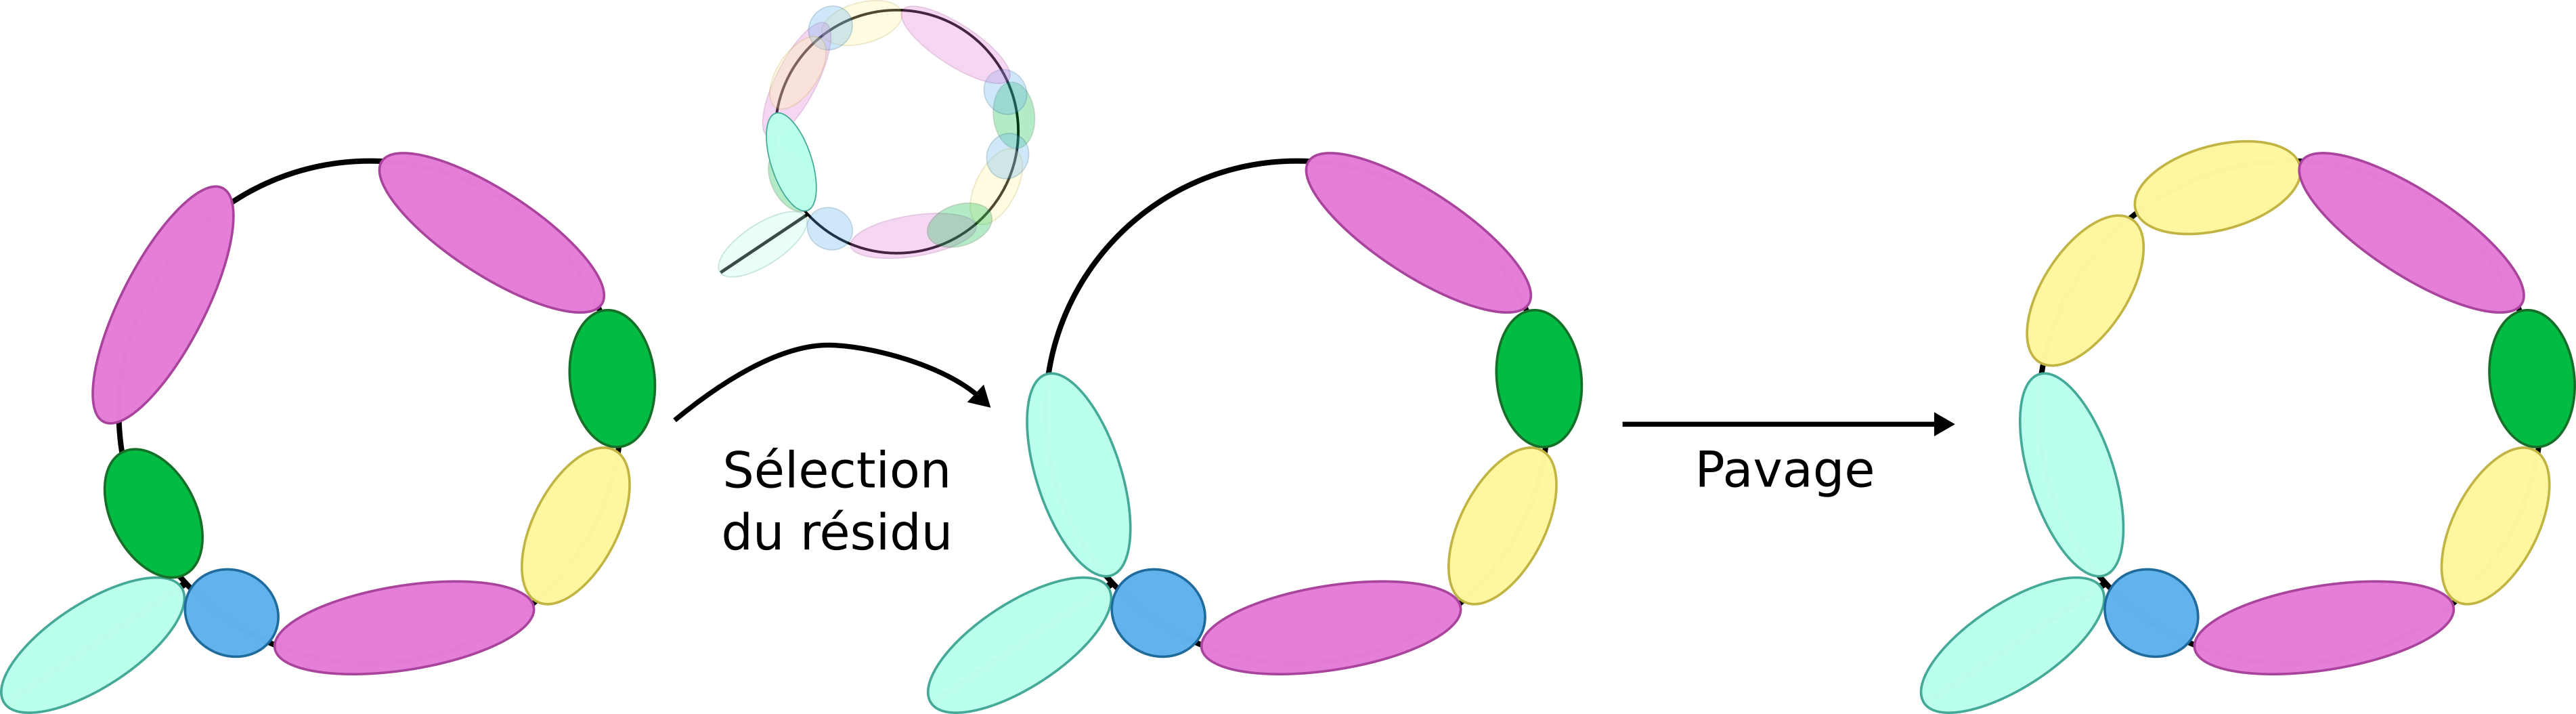
\includegraphics[width=350px]{Figures/s2m/pavage/modulation.png}
    \caption{\label{modulation}Modulation de la solution initiale (à gauche) pour obtenir une solution optimale (à droite) en remplaçant des monomères choisis par d'autres laissés de côté après l'étape de pavage.
    En haut, les monomères issus de la recherche.
    C'est parmi ceux-ci que la modulation va choisir des remplaçants de la solution actuelle.}
  \end{center}
\end{figure}

\paragraph{}
\begin{algorithm}[H]
  \caption{Algorithme de modulation du pavage}
  \KwData{Un peptide requête $P$ et une liste de résidus $RES$ pavés sur $P$ lors de la phase d'isomorphisme et triés par
  l'algorithme glouton, une pré-solution $SOL$ et un ensemble $INT$ de résidus interdits d'utilisation.}
  \KwResult{$SOL$, un sous-ensemble de $RES$ de pièces non chevauchantes sélectionnées par la modulation}
  
  $r \gets$ Premier élément de $RES$ couvrant au moins un atome non couvert et n'étant pas présent dans $INT$\;
  \If {$r$ n'existe pas} {
    \KwRet Impossible\;
  }
  Soit $SUPPR$ une liste de résidus\;
  \For {$r_i \in SOL$} {
    \If {$r_i$ chevauche $r$} {
      Ajouter $r_i$ à $SUPPR$\;
      Supprimer $r_i$ de $SOL$\;
      Ajouter $r_i$ à $INT$\;
    }
  }
  
  Lancer un pavage pour compléter $SOL$\;
  
  \If {$SOL$ couvre $P$ à 100\%} {
    \KwRet $SOL$\;
  }
  
  $SOL \gets$ Modulation récursive\;
  
  \If {$SOL = $ Impossible} {
    Supprimer $r$ de $SOL$\;
    Ajouter $r$ dans $INT$\;
    \For {$r_i \in SUPPR$} {
      Enlever $r_i$ de $INT$\;
      Ajouter $r_i$ à $SOL$\;
    }
  }
  
  \KwRet $SOL$\;
\end{algorithm}


\paragraph{}L'algorithme permet d'explorer toutes les solutions possibles jusqu'à obtenir la meilleure. Le problème majeur
est que si une solution parfaite n'existe pas, l'algorithme de modulation va parcourir tout l'arbre des solution et l'exécution
ne sera pas plus rapide que l'exécution d'une résolution de MIP. Rappelons que le pavage glouton effectue des choix que nous
supposons pertinents. Il n'est donc normalement pas nécessaire de modifier la solution en profondeur pour 
obtenir l'idéal. Si la solution n'est pas trouvée rapidement, il y a fort à parier que la solution idéale n'existe
pas. On peut donc limiter la profondeur de notre algorithme de modulation en proposant de considérer qu'il n'y a pas de solution
possible après $i$ appels récursifs ($i$ paramétrable).


\subsection{Recherche approximative (light)}

\label{light_p}

\paragraph{}Suite à des variations de composition ou de structure survenant dans certains résidus quelques polymères ne sont pas
découpés correctement en utilisant les algorithmes précédents. Il y a essentiellement deux cas pour lesquels l'isomorphisme
ne fonctionne pas. Dans un premier cas, nous avons a faire à un monomère ionisé au sein du peptide. Dans ce cas, il se peut qu'un
proton ait été perdu et lors de la phase d'isomorphisme, la fonction de matching d'étiquettes ne répond plus correctement car il
manque un décorateur $H$ sur l'un des atomes. Dans le second cas c'est encore l'isomorphisme qui ne reconnaît pas un résidu car
celui-ci est intégré sous une forme tautomérique (voir figure \ref{tautomer}).
Un tautomère de molécule est un isomère structurel de cette molécule.
C'est à dire que la molécule tautomérique contient l'ensemble des atomes de la molécule initiale  mais certains
de ces atomes ne sont plus liés aux même voisins. Dans le cas d'un tautomère, c'est un noyau d'hydrogène qui se déplace et change
de voisin. Cette charge positive déplacée est compensée par une charge négative qui se déplace dans l'autre sens. Ce déplacement
d'électron se concrétise par le déplacement d'un liaison double.

\begin{figure}
  \begin{center}
    \includegraphics[width=300px]{Figures/s2m/residues/tautomers.png}
    \caption{\label{tautomer}Tautomérie d'une molécule}
  \end{center}
\end{figure}

\paragraph{}Les deux transformations présentées ont pour point commun de ne pas modifier en profondeur la structure des molécules.
Dans les deux cas seuls les ``décorateurs'' des étiquettes sont modifiés (hydrogènes et arité de liaison).
Le moyen simple de reconnaître ce type de molécule est alors d'oublier ces décorateurs lors de la phase d'isomorphisme.
Dès lors les résidus sont reconnus quel que soient leurs variations sur les hydrogènes ou les liens.
Cette modification ne fait pas varier la qualité des résultats sur les NRP car les monomères utilisés différent entre eux au delà des atomes d'hydrogène.
Bien que très séduisante cette méthode pose un problème de temps de calcul.
La plupart des monomères NRP ne contiennent que des atomes C N O et H.
Ne pouvant plus utiliser les H comme décorateurs et en rendant les liens indifférents les uns des autres, le nombre d'étiquettes différentes chute à 9.
Il est donc compréhensible que le temps de calcul augmente beaucoup.

\paragraph{}La solution est une nouvelle fois hybride.
Dans un premier temps, nous cherchons rapidement une solution en effectuant un
isomorphisme contenant toutes les étiquettes (isomorphisme {\em strict}), puis en effectuant un pavage.
Dans un second temps si aucune solution complète n'est trouvée, nous relançons tout le processus en commençant par
une nouvelle phase d'isomorphisme sans les décorateurs (isomorphisme {\em light}).
Cette seconde phase d'isomorphisme est effectuée localement autour des zones qui ont posé problème lors du premier tour de 
l'algorithme.
Cette algorithme en deux temps traite rapidement tous les cas simples avec des sous algorithmes efficaces puis
de revenir sur les cas plus difficiles avec des algorithmes plus sensibles.

\subsubsection{Vue globale des algorithmes}

\begin{figure}
  \begin{center}
    \includegraphics[width=300px]{Figures/s2m/algo/s2m.pdf}
    \caption{\label{global_s2m}Schéma global de Smiles2Monomers (TODO : refaire avec les deux alternatives)}
  \end{center}
\end{figure}

\paragraph{}Tout au long cette partie, nous avons présenté par morceaux les différentes parties de Smiles2Monomers.
Nous rassemblons ici tous les morceaux au sein d'un schéma global (figure \ref{global_s2m}).
Le première partie du schéma (au dessus des pointillés) est composée des deux phases de pré-calcul (voir \ref{index_p}).
Cette étape de pré-calcul est lourde en temps mais n'est à effectuer qu'une seule fois.
Chacune des deux phases de cette étape se déroule en temps exponentiel mais reste calculables grâce à la petite taille des
données.
La partie principale de s2m possède deux alternatives algorithmiques.
Dans les deux cas, l'algorithme commence par une phase de recherche d'isomorphismes (voir \ref{isomorphisme_p}) afin de connaître les résidus candidats à la composition du polymère.
Ensuite vient la phase de pavage effectuée soit par une résolution de MIP (voir \ref{MIP_p}) soit par une heuristique de pavage (voir \ref{TM_p}).
Enfin, pour les cas plus difficile, nous effectuons plusieurs passes de recherche d'isomorphismes light (voir \ref{light_p}) et de nouveaux pavages.

L'algorithme global est paramétrable.
Pour le précalcul, nous pouvons fixer la variable $k$ qui définira la taille de chaîne calculée avec le modèle markovien.
Nous rappelons encore une fois que cette taille n'aura pas d'influence sur le résultat mais uniquement sur le temps de calcul.
Pour la partie recherche, nous devrons choisir le nombre de fois où nous effectuerons la ``boucle light''.
Ce paramètre est appelé ``retry'' dans le logiciel (nombre de fois où l'on ré-exécute la boucle).
Si nous optons pour la méthode heuristique de modulation, il est également nécessaire de définir une profondeur maximale de modulation (paramètre appelé ``modulation'' dans le logiciel).
L'influence de ces paramètres sur l'exécution de l'algorithme sera étudiée durant la partie résultats.




\section{Résultats et interprétations}

\subsection{Jeux de données}

\subsubsection{Les constituants des jeux de données}

\paragraph{}Nous souhaitons connaître la pertinence des annotations issues de s2m.
Pour cela, nous avons construit deux jeux de données tests, au sein desquels les annotations attendues sont déjà connues.
Ces bases de test sont composées de polymères comprenant leur SMILES, représentation de leur structure atomique ainsi que de l'annotation attendue (un graphe monomérique).
Pour les entrées de s2m, nous constituons une base de monomères pour chacun des jeux de données.
s2m pré-calculera les indexes pour chaque base de monomère puis s'exécutera sur chaque polymère.
L'annotation de sortie sera alors comparée à l'annotation préexistante pour en définir la qualité.


\subsubsection{Premier jeu de données : Norine}

\paragraph{}Puisque le déclenchement de ce travail est dû à la volonté d'accroitre le nombre d'annotations de NRP dans Norine, le premier jeu de données sera logiquement constitué de polymères non ribosomiques déjà annotés issus de cette base.
Toutes les entrées de Norine sont accompagnées d'annotations monomérique et c'est d'ailleurs ce qui fait la force de cette base.
Nous avons donc extrait tous les NRP pour lesquels un SMILES était renseigné pour constituer un jeu de polymères test.
La base de monomères est quant à elle constituée de l'ensemble des monomères connus et présents dans Norine.


%Citations :
%· The chemical component dictionary: complete descriptions of constituent molecules in experimentally determined 3D macromolecules in the Protein Data Bank
%· The Protein Data Bank
\subsubsection{Second jeu de données : The Chemical Component Dictionary (CCD)}

\paragraph{}CCD~\cite{westbrook_chemical_2015} est une sous partie de la base de données PDB~\cite{berman_protein_2000} (Protein Data Bank).
Cette base regroupe toutes les petites molécules présentes dans PDB.
Parmi celles-ci se trouvent de nombreux polymères annotés ainsi que les monomères les constituant.
L'avantage de cette base est que toute molécule y étant présente est accompagnée de son smiles.
En extrayant les molécules annotées comme polymères, nous avons constitué un second jeu de données.
Pour constituer la base de monomères dont s2m à besoin en pré-traitement, il nous a suffit d'extraire les molécules présentes dans les annotations polymériques.


\subsubsection{Résumé sur les données}

Les données de validation seront composées de deux jeux distincts.
D'un côté les polymères extraits de Norine seront au nombre de 343.
Les données NRP seront accompagnées des 533 monomères de la base.
Le second jeu est issu de la base CCD et comporte 378 polymères et 507 monomères issus des annotations.
Il est à noté qu'aucun des polymères présent dans une base n'est présent dans l'autre et que seuls 63 monomères sont communs.
Ces monomères identiques sont en très grande majorité des acides aminés classiques et leurs variants proches.

\begin{figure}[!ht]
  \begin{center}
    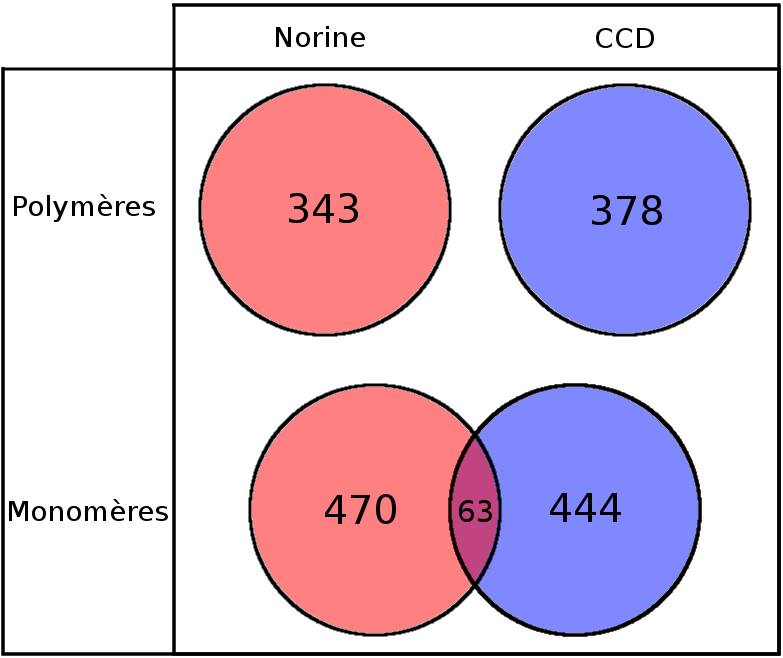
\includegraphics[width=250px]{Figures/s2m/results/data.png}
    \caption{\label{data}Répartition des données de validation}
  \end{center}
\end{figure}



\subsection{Profil d'un résultat}

\paragraph{}s2m permet de générer des résultats sous différents formats.
Il est possible par exemple de générer un format textuel json permettant facilement de recharger ces résultats dans d'autres logiciels.
Lorsque nous présenterons un résultat ici, nous le présenterons via le format graphique html.

\begin{figure}[!ht]
  \begin{center}
    \includegraphics[width=450px]{Figures/s2m/results/apicidinC.png}
    \caption{\label{s2m_HTML}Le résultat HTML de l'exécution de s2m sur l'apicidine C}
  \end{center}
\end{figure}

\paragraph{}Une page de résultat peut être décomposée en 3 parties (voit figure \ref{s2m_HTML}).
En haut à gauche se trouve l'image du polymère étudié, colorée selon les monomères qui y sont présents.
C'est l'information la plus parlante visuellement car elle permet d'immédiatement interpréter les résultats.

Sous l'image du peptide se trouvent trois listes de monomères.
La première liste correspond aux monomères découverts dans la structure atomique par s2m et que l'on sait être justes grâce aux annotations déjà connues.
Le seconde liste correspond également aux monomères découverts par s2m mais qui cette fois-ci ne sont pas présent dans l'annotation initiale.
La dernière correspond aux monomères qui sont présent dans l'annotation mais qui n'ont pas été trouvés par s2m.

La dernière partie de la figure représente les informations générales sur le polymère.
Tout d'abord, il y a le nom du polymère puis les statistiques sur celui-ci.
La première statistique est le taux de couverture atomique (Coverage).
Cette valeur donne le ratio des atomes annotés par s2m comme faisant partie des monomères trouvés par le nombre d'atomes du polymère.
La seconde valeur donne également un ratio d'atomes mais uniquement pour les atomes correctement annotés.
Cette valeur ne prend en compte que les atomes faisant partie des monomères de la première des trois listes.
Lors de la présentation des résultats qui suivront, nous ferons toujours attention de bien mentionner si les chiffres sont des comptages monomériques ou des comptages atomique.
Les pourcentages de l'un à l'autre peuvent être fort différents dû à la variabilité du nombre d'atomes composant les monomères.





\subsection{Choisir les paramètres}

\paragraph{}Nous allons tout d'abord nous poser la question de comment choisir les bons paramètres pour effectuer nos tests.
Nous reviendrons d'abord sur la façon de fixer le paramètre d'apprentissage pour le précalcul.
Rappelons que de ce paramètre découlera le temps de calcul pour les peptides mais que la qualité des résultats ne variera pas.
Puis nous parlerons de la qualité des résultats obtenus en exécutant le programme pour plusieurs paramètres.
Enfin nous étudierons le temps de calcul pour estimer les rapports temps/qualité et ainsi pouvoir recommander les meilleurs calibrations de l'outil.

\subsubsection{Choisir le k du précalcul}

\paragraph{}Pour rappel, l'isomorphisme de sous graphe est effectué à partir de chaînes pré-calculées afin d'optimiser le temps de recherche (voir partie \ref{index_markov}).
Ces chaines sont formées de deux sous-parties.
La première, de taille k, est optimale sur la base d'apprentissage.
La seconde est générée de manière gloutonne.

Ici, nous allons faire varier ce paramètre k et tester les temps de calcul sur les jeux de données.
Pour ne pas parasiter la mesure du temps, nous allons désactiver toutes les autres optimisations logicielles qui augmentent l'efficacité.

\begin{figure}[!ht]
  \begin{center}
    \includegraphics[width=450px]{Figures/s2m/results/k.png}
    \caption{\label{k_graph}Évaluation de l'efficacité d'apprentissage des chaînes.
    A gauche : représentation du temps de recherche moyen d'une chaîne dans un peptide pour plusieurs valeurs de k.
    A droite : temps d'apprentissage pour tous les monomères pour plusieurs valeurs de k.}
  \end{center}
\end{figure}

\paragraph{}Observons les résultats sur le schéma \ref{k_graph}.
Le graphique de gauche représente le temps d'exécution moyen d'un isomorphisme (ie recherche d'une chaîne dans un peptide) en fonction de k.
Le graphique de droite représente le temps d'apprentissage en fonction du k.

Quels que soient les valeurs de k, la recherche est très rapide.
On parle ici en centièmes de millisecondes.
Lorsque la chaîne est entiérement générée de manière gloutonne, chaque isomorphisme prend environ 8 centièmes de ms.
Ce temps descend à 5 centièmes à partir d'un k valant 3.
Ce résultat est très intéressant car il nous montre que seuls les 3 premiers n\oe{}uds sont utiles pour l'optimisation des chaînes.
Les monomères non trouvables dans une peptide donné (même ceux étant constitués de plusieurs dizaines d'atomes), peuvent déjà tous être éliminés après 3 atomes si les chaînes sont correctement formées.
Il n'est donc pas nécessaire de précalculer (sur nos données) des chaînes avec un k supérieur à 3.
Ce précalcul fait gagner près de 35\% d'efficacité à chaque recherche de SI.


\subsubsection{Mesures}

\paragraph{}Classiquement, lorsque l'on souhaite évaluer les résultats d'une prédiction, on utilise les statistiques découlant des vrai/faux positifs/négatifs.
Commençons par définir chacune de ces catégories dans notre cas :
\begin{itemize}
 \item Vrai positif (VP) : Un vrai positif est obtenu lorsque le résultat de la prédiction est identique au résultat attendu.
Dans notre cas, une annotation peptidique est un VP si tous les monomères présents dans l'annotation de s2m sont également présent au sein de l'annotation du jeu de test et inversement.
Nous aurons donc une couverture et un correctness de 100\%.
 \item Faux positif (FP) : Un faux positif est obtenu lorsque le résultat de la prédiction parait correct mais qu'il diffère du résultat attendu.
Dans notre cas, une annotation est un FP si tout ses atomes sont couverts par l'annotation mais que celle-ci diffère du jeu test.
Nous aurons donc une couverture de 100\% et un correctness inférieur à 100\%
 \item Faux négatif (FN) : Un faux négatif est obtenu lorsque le résultat ne parait pas correct alors qu'il est possible de l'obtenir.
Dans notre cas, une annotation est un FN lorsque nous n'arrivons pas à produire une annotation complète du peptide.
C'est à dire que nous aurons une couverture et une correctness inférieure à 100\%.
 \item Vrai négatif (VN) : Un vrai négatif est obtenu lorsque le résultat ne parait pas correct et qu'il n'est pas possible d'en obtenir un.
Dans notre cas, si les annotations test sont correctes, ce n'est pas possible.
Il est toujours possible d'obtenir une annotation couvrante vu qu'elles sont toutes présentes dans le jeu test.
\end{itemize}


\subsubsection{Exécutions sur les jeux de données}

\label{resultats_s2m_p}

\paragraph{}Pour le choix des paramètres, nous n'allons pour le moment pas prendre en compte le temps d'exécution.
Les but ici est d'exposer uniquement la qualité des résultats.
Pour cela nous allons prendre comme indicateurs la couverture atomique moyenne, le correctness atomique moyen et les taux de VP/FP/FN.
Nous allons faire varier le paramètre du nombre de tour de la boucle light ainsi que la profondeur de modulation pour le pavage avec modulation.
Nous testerons également les deux algorithmes algorithmes de pavage (MIP et heuristique).

\begin{table}[!ht]
  \centering
  \begin{tabular}{|c|c|c|c|c|c|c|c|c|}
    \hline
    & \multicolumn{4}{c|}{Heuristique} & \multicolumn{4}{c|}{MIP} \\
    \hline
    Params (R-M) & FN & FP & VP & Sensibilité & VP & FP & FN & Sensibilité \\
    \hline
    1 - 1 & 69 & 56 & 217 & 0.759 & 243 & 68 & 31 & 0.887 \\
    \hline
    2 - 1 & 69 & 56 & 217 & 0.759 & 243 & 68 & 31 & 0.887 \\
    \hline
    1 - 2 & 30 & 62 & 250 & 0.893 & 243 & 68 & 31 & 0.887 \\
    \hline
    2 - 2 & 26 & 63 & 253 & 0.907 & 243 & 68 & 31 & 0.887 \\
    \hline
    3 - 3 & 26 & 63 & 253 & 0.907 & 243 & 68 & 31 & 0.887 \\
    \hline
  \end{tabular}
  \caption{\label{nor_results}Résultats de s2m sur les données de Norine.
  Dans la première colonne se trouvent les binômes des valeurs des paramètres retry et modulation}
\end{table}

\begin{figure}[!ht]
  \begin{center}
    \includegraphics[width=450px]{Figures/s2m/results/Norine.png}
    \caption{\label{nor_graph}Diagramme en barre des résultats sur Norine}
  \end{center}
\end{figure}

\begin{table}[!ht]
  \centering
  \begin{tabular}{|c|c|c|c|c|c|c|c|c|}
    \hline
    & \multicolumn{4}{c|}{Heuristique} & \multicolumn{4}{c|}{MIP} \\
    \hline
    Params (R-M) & FN & FP & VP & Sensibilité & VP & FP & FN & Sensibilité \\
    \hline
    1 - 1 & 45 & 44 & 289 & 0.865 & 310 & 56 & 12 & 0.963 \\
    \hline
    2 - 1 & 45 & 44 & 289 & 0.865 & 310 & 56 & 12 & 0.963 \\
    \hline
    1 - 2 & 10 & 50 & 318 & 0.970 & 310 & 56 & 12 & 0.963 \\
    \hline
    2 - 2 & 9 & 51 & 318 & 0.972 & 310 & 56 & 12 & 0.963 \\
    \hline
    3 - 3 & 9 & 51 & 318 & 0.972 & 310 & 56 & 12 & 0.963 \\
    \hline
  \end{tabular}
  \caption{\label{ccd_results}Résultats de s2m sur les données de CCD.
  Dans la première colonne se trouvent les binômes des valeurs des paramètres retry et modulation}
\end{table}

\begin{figure}[!ht]
  \begin{center}
    \includegraphics[width=450px]{Figures/s2m/results/CCD.png}
    \caption{\label{ccd_graph}Diagramme en barre des résultats sur CCD}
  \end{center}
\end{figure}


\paragraph{}Comme nous voyons au sein des tableaux \ref{nor_results} et \ref{ccd_results}, l'algorithme de pavage par optimisation linéaire n'est pas du tout sensible au changement de paramètres.
Ceci s'explique par le fait qu'il n'a besoin que d'une seule phase light pour parvenir à son optimal local.
En effet, dans certains cas, le problème et tout de suite résolu après la première phase de pavage succédant l'isomorphisme light car toutes les briques ont été correctement découvertes.
Dans les autres cas, l'algorithme du MIP a tellement cherché à optimiser les nombre d'atomes couverts à la suite du premier pavage, que la solution intermédiaire est trop distante de la vraie solution pour pouvoir être rattrapée.

Pour le pavage heuristique, la sensibilité aux paramètres est bien différente.
On peut voir que l'augmentation du nombre de modulations déclenche une augmentation du nombre de VP.
Le nombre de vrais positifs augmente significativement en passant le paramètre de 1 à 2.
Cette sensibilité s'explique par le fait que la solution optimale et la solution gloutonne ne sont pas immédiatement voisines.
Il est souvent nécéssaire de déplacer non pas un mais deux monomères pour atteindre l'optimal.
Le paramètre de nombre de boucle light n'a que très peu d'influence et vient seulement compléter 3 résultats sur les données Norine et un seul sur les données de CCD.

\paragraph{}En comparant les résultats des deux algorithmes, on s'aperçoit que l'algorithme comprenant l'heuristique de pavage obtient de meilleurs résultats (pour une modulation $\ge$ 2) que l'algorithme incluant un pavage exact.
A nouveau, ce résultat s'explique par le fait que le pavage exact va trop loin dans l'optimisation.
Si aucune solution totalement couvrante n'est possible avec les résidus issus de l'isomorphisme strict, alors le pavage maximal exact ira parfois créer des solutions optimisées globalement mais farfelues.
Dans ce cas, la recherche de résidus par isomorphisme light sert peu car les trous dans l'annotation ont été déplacés par l'optimisation.
Il n'est souvent plus facilement possible de construire l'annotation.

\paragraph{}Au final, les résultats obtenus sont strictement meilleurs en utilisant l'heuristique gloutonne de pavage avec une modulation de profondeur 2 et deux phases de recherche light.
Nous ne nous attendions pas à ces résultats et la sur-optimisation du pavage par MIP nous a surprit mais 


\subsubsection{Temps de calcul global}

\begin{figure}[!ht]
  \begin{center}
    \includegraphics[width=400px]{Figures/s2m/results/temps.png}
    \caption{\label{temps_general}Temps d'exécution moyen par peptide (en ms) en utilisant les deux pavages différents et différents parêtres pour chacun d'eux.}
  \end{center}
\end{figure}

\paragraph{}Pour choisir les paramètres il ne faut pas prendre que les résultats en considération mais également le temps qu'il faut pour les générer.
Pour cela, nous avons effectué une analyse comparative des algorithmes en utilisant les différents paramètres cités précédemment.
Comme nous pouvons le remarquer sur le schéma \ref{temps_general}, l'heuristique de pavage permet un temps d'exécution beaucoup plus faible le pavage MIP (Excepté pour le pavage heuristique 3-3 qui n'a pas d'importance puisqu'il n'apporte pas de qualité).
Ce résultat était attendu mais l'écart flagrant vient confirmer la nécessité d'utiliser l'heuristique de pavage plutôt que le MIP.
Après les contres-performances du pavage MIP, à la fois en qualité de résultats qu'en temps d'exécution, nous excluons cet algorithme des recommandations d'utilisation.

\paragraph{}Comparons désormais les temps d'exécution pour l'heuristique en fonction des paramètres passés au programme.
Le pramètre du nombre de boucles light semble avoir le plus d'influence sur le temps d'exécution.
Nous pouvons expliquer cette augmentation par la difficulté rencontrée par l'algorithme d'isomorphisme lorsque peu d'étiquettes sont présentes.
Répéter l'opération plusieurs fois multiplie logiquement le temps d'exécution.

Si l'on regarde bien les temps d'exécution on peut également s'apercevoir que l'augmentation du second paramètre (la profondeur de modulation) permet de diminuer le temps d'exécution pour un nombre de boucles light fixe.
En effet, plusieurs solutions sont bloquées par le manque de profondeur de modulation et non pas par le nombre de boucles.
Les monomères pour reconstruire le peptide ont tous été trouvés mais la solution gloutonne n'est pas immédiatement voisine de la solution optimale.
Effectuer une modulation plus poussée permet d'arriver beaucoup plus vite à une solution.

\paragraph{}Pour conclure cette partie  sur la sélection des paramètres, nous pouvons dire qu'il faudra toujours privilégier l'utilisation de l'algorithme de pavage heuristique par rapport au pavage MIP.
Cependant, il ne faut pas utiliser n'importe quels paramètres.
Pousser les paramètres de modulation ou de nombre de boucle à 3 ou au delà est parfaitement inutile en terme de résultats et consommera énormément de temps.
Utiliser un paramètre de modulation de 1 sera également une erreur puisque la qualité des résultats ne sera pas au rendez-vous.
Il reste finalement deux alternatives intéressantes.
Soit nous privilégions la qualité à la vitesse et nous réglons les deux paramètres à la valeur 2, soit nous acceptons de perdre quelques pourcents de bons résultats au profit de 30\% d'économie de temps en réglant uniquement la modulation à 2.



\subsection{Répartition des temps de calcul et analyse}

\paragraph{}Maintenant que nous avons choisi les paramètres analysons attentivement chacune des étapes pour comprendre les points critiques et préparer de futures améliorations.
Pour cela, nous avons exécuté le logiciel sur tous les peptides des jeux test en utilisant un pavage heuristique, une valeur de k de 3, une modulation de 2 et un nombre de tour de boucle de 2.
Pour chacun des peptides, nous avons stocké séparément les temps pour l'isomorphisme strict, le light, le pavage et la modulation.
Les résultats sont affichés sur la figure \ref{temps_calcul}.

\begin{figure}[!ht]
  \begin{center}
    \includegraphics[width=450px]{Figures/s2m/results/temps_detail.png}
    \caption{\label{temps_calcul}Temps d'exécution de s2m pour un extrait aléatoire de 350 molécules.
    Les données ont été tronquées au delà de 50ms pour ne pas écraser le graphique.}
  \end{center}
\end{figure}

\paragraph{}Certains points de la figure ont été tronqués car ils écrasaient les résultats.
15 valeurs sur les 350 ont été redescendues à 50ms alors que certaines allaient jusqu'à plusieurs centaines de ms (Le point max atteint 1s à lui seul).
On distingue nettement deux comportements différents sur cette courbe.
Soit les peptides ont été complètement analysés à la suite d'une seule passe de pavage suite (celle succédant la recherche stricte) ; dans ce cas, le temps d'exécution épouse une courbe qui augmente progressivement avec le nombre d'atomes ; soit le matching light et la modulation qui suit entrent en action et le temps devient fortement dépendant de la topologie du peptide (tous les points disparates).

Pour ce qui est de la première catégorie de peptide, on peut voir que la quasi-intégralité du temps est dépensé sur la recherche d'isomorphismes de sous graphe.
Comme nous le supposions au début de ce projet, les isomorphismes sont des goulots d'étranglement du fait de la complexité des algorithmes de résolution.
Pour quelques peptide, le temps est complété par une phase de modulation qui ne prend que quelques millisecondes.
Dans le pire des cas, le temps est doublé par cette modulation.
L'étape de pavage ne prend jamais plus de 3ms et n'est pas un problème pour le temps d'exécution.

Pour les points de la seconde catégorie, c'est encore l'étape de recherche qui prend le plus de temps.
Sauf que cette fois-ci, ce sont les étapes de recherche light qui prédominent le temps de calcul.
Comme nous l'avions évoqué lors de la présentation de cette amélioration, le manque d'étiquettes disponibles diminue fortement l'efficacité de l'algorithme.
En moyenne, un isomorphisme light est de 10 à 100 fois plus lent qu'un strict.
De plus, les cas qui posent problème sont très souvent accompagnés de longues exécutions de modulation.
Cependant, ce temps d'attente vaut le coup puisque la majorité des cas sont résolus.
Sur l'extrait des peptides ici présent, seules 20 d'entre eux finissent sur des impasses.
Toutes les autres exécutions s'arrêtent en obtenant 100\% de couverture.

\paragraph{}Pour finir cette analyse des temps de calcul individuels, nous allons parler des cas extrêmes.
Ces cas pathologiques masquent les réelles performances du logiciel.
La moyenne de temps d'exécution globale est de 18ms par peptide mais lorsque nous retirons les 15 cas qui débordent de la figure, cette moyenne chute à 10ms.
À eux seuls, ces 15 peptides représentent plus de la moitié du temps d'exécution du logiciel.
Le cas le plus critique à lui seul représente un cinquième du temps d'exécution total (plus de 1s).
Ce qu'il faut conclure de cela est qu'il faut éviter d'utiliser des boucles light sur des données dont on ne connait pas grand chose.
Si nous souhaitons par exemple analyser à l'aveugle un très grand nombre de molécules, il est préférable de se restreindre à une utilisation basique du logiciel, quitte à venir affiner les résultats intéressants par la suite.








\subsection{Analyse des résultats}

\paragraph{}Pour analyser les résultats, nous avons exécuté s2m avec l'algorithme de pavage heuristique.
La modulation est réglée à 2 de profondeur et le nombre de tours de boucle à 2 également.s
Vous pourrez trouver tous les résultats sur les polymères testés à ces adresses :
- CCD : www.TODO.com
- Norine : www.TODO.com


\paragraph{}Revenons sur les chiffres qui ont été présentés dans le tableau TODO.
Environ 74\% des annotations peptidiques issus de Norine et 85\% de celles de CCD sont entièrement retrouvées par le logiciel.
Mais il faut se rappeler que les annotations ne sont plus considérées comme correctes dès lors qu'au moins un monomère est faux.
En regardant le taux d'atomes correctement attribués au sein des peptides, le taux de réussite augmente à plus de 93\% pour les annotations de Norine et plus de 98\% pour CCD.

Cependant, même ces très bons taux de réussite ne sont pas représentatif de la qualité des annotations.
En effet, en analysant les résultats de plus près, nous nous sommes aperçu qu'il était possible de détecter des erreurs au sein des bases de données utilisées pour les tests.
Analysons ensemble plusieurs cas afin de comprendre les raisons de ces erreurs.


\subsubsection{Des peptides aux structures atomiques fausses}

\begin{figure}[!ht]
  \begin{center}
    \includegraphics[width=400px]{Figures/s2m/results/s2m_enniati.png}
    \caption{\label{s2m_enniati}Résultat de s2m pour l'enniatin I.
    Deux monomères sont annotés faux ce qui nous mène à dire qu'une erreur s'est glissée soit dans le SMILES de la molécule soit dans l'annotation monomérique.}
  \end{center}
\end{figure}

\paragraph{}Beaucoup d'annotations fausses proviennent d'erreurs de structures atomiques pour les peptides.
Prenons l'exemple de l'``enniatin I'' (voir figure \ref{s2m_enniati}).
L'annotation en sortie de s2m présente une couverture de 100\% mais un correctness de 66\%.
En regardant les 3 listes de monomères, on peut s'apercevoir que l'annotation attendue comporte deux monomères nommés Hmp alors que le logiciel trouve deux 4Me-Hva.
Les deux monomères se ressemblant et il est fort probable que, soit l'annotation monomérique, soit l'annotation atomique ait été mal entrée.
Pour comprendre l'erreur, remontons les sources des données.
Sur la page Norine de la molécule, nous trouvons un lien vers Pubchem pour nous permettre d'obtenir la structure atomique et un lien vers la publication qui nous permet d'obtenir la structure monomérique.

\paragraph{TODO : Figure structures PubChem et publi}

\paragraph{}En regardant la molécule présente sur PubChem, nous pouvons constater que c'est effectivement la structure atomique qui a été utilisée pour le test.
En lisant désormais la publication, on s'aperçoit que la structure monomérique correspond à ce qui est présent sur Norine.
Accompagnant cette annotation monomérique est présent un schéma de la structure atomique venant confirmer la structure monomérique.
Sans aucun doute, l'erreur provient des données issues de PubChem.
A priori le lien PubChem entré sur Norine n'est pas le bon et pointe vers un peptide similaire.

\paragraph{}Nous n'avons pas fini de traiter manuellement toutes les données issues de s2m mais au moins 50\% des erreurs sont de ce type.


\subsubsection{Des monomères aux structures atomiques fausses}

\label{dolastatin_p}

\paragraph{TODO : Figure de la dolastatin 10}

\paragraph{}Lorsque le taux de couverture de l'annotation issue de s2m est inférieur à 100\%, par définition, au moins un monomère n'a pu être trouvé.
Il est possible que ce monomère n'ait jamais été répertorié, que la structure atomique du peptide soit incorrecte ou que la structure d'un monomère le soit également.
Dans le cas de l'annotation de la dolastatin, c'est une erreur de structure atomique qui s'est glissée dans la base Norine.
Le monomère Dap qui est sensé être présent n'est pas reconnu car l'atome d'azote n'est pas placé au même endroit au sein du monomère seul et du monomère dans le peptide.
En cherchant sur Norine on peut s'apercevoir qu'aucun autre peptide de la base ne comporte ce monomère, ce qui veut dire qu'il a été ajouté spécifiquement pour ce peptide.
Donc, le changement de structure du monomère n'est probablement pas du à une modification de la molécule mais plutôt à une erreur d'annotation.
En parcourant l'article qui publia le peptide et la structure atomique présente sur PubChem, on s'aperçoit que c'est une erreur uniquement présente sur Norine.


\subsubsection{Erreurs d'annotations}

\paragraph{TODO : Figure de la fengycine A (ci.inria)}

\paragraph{}Il arrive parfois que des molécules soient trompeuses.
En entrant à la main les annotations, il est possible de confondre un monomère avec un de ses dérivés proches.
C'est ce qui est arrivé avec la fengycine A.
L'annotation effectuée par s2m détecte un monomère Gln alors que l'annotation présente dans Norine détecte un Glu.
En effectuant à nouveau toutes les opérations de vérification de la structure atomique et monomérique, on s'aperçoit rapidement que l'article donne raison à s2m.
Cette fois-ci c'est l'annotation monomérique présente dans Norine qui est à changer pour obtenir une information juste.


\subsubsection{Les équivalences}

\paragraph{TODO : Schéma cyclotheonamide E}

\paragraph{}Le dernier type d'erreurs d'annotations commises par s2m est strictement dut aux algorithmes utilisés pour le pavage.
C'est un problème d'annotations équivalentes.
Comme nous le voyons sur le schéma de la ``cyclotheonamide E'', le peptide est couvert à 100\%.
De plus, l'annotation présente dans Norine propose deux monomères visuellement très proches des monomères suggérés par s2m.
En regardant dans le détail, on peut observer que c'est un problème dut à une formylation entre deux monomères.
L'un des deux monomère à été formylé, ce qui fait qu'un groupement C=O est présent entre les monomères Arg et Ile du peptide.
L'un des monomères à donc été modifié mais il pourrait a priori s'agir de l'un comme de l'autre.
Dans les deux cas, l'annotation qui en résulte reste couvrante à 100\%.
N'ayant aucun moyen algorithmique de faire la différence, ici s2m a choisit la première solution sur laquelle il est tombé.
Pour connaître l'annotation réelle, il faut remonter à la production du peptide et comprendre les mécanismes de modifications de monomère ici en jeu.
Cette erreur est présente moins d'une dizaine de fois dans les données déjà vérifiées et ne pourra pas être corrigée sans ajouter plus d'information en entrée de s2m.


\subsubsection{Les analyses d'erreur pour CCD}

\paragraph{TODO : Figure équivalence obvious}

\paragraph{}Durant toutes les analyses, je ne me suis attardé que sur des erreurs issues des peptides de Norine.
Pour nous, il est très facile de vérifier toutes les informations de cette base car de nombreux liens vers les origines des données sont présents en son sein.
Pour les données issues de CCD, nous détectons le même genre de problème que dans Norine mais il est très difficile de les analyser en profondeur.
Nous avons accès aux structures mais difficilement à des publications associées.
Nous pouvons donc détecter la présence d'erreurs mais sans forcément pouvoir expliquer pourquoi.
Seules les erreurs dues aux équivalences sont facilement détectables (voir par exemple TODO).





\chapter{Vers un enrichissement de Norine}

\section{Norine}

\subsection{Généralités}

\paragraph{}Nous avons déjà plusieurs fois abordé la base de données Norine au sein de ce manuscrit mais nous allons ici décrire en détail son fonctionnement.
Norine à été créée durant la thèse de Ségolène Caboche (2006-2009) dans le but de centraliser l'information sur les NRP.
Avant cette base, il n'existait rien permettant de croiser directement les données NRP.
Les structures atomiques et monomériques de NRP étaient publiées dans des articles scientifiques puis parfois mises en ligne au sein de bases généralistes.
Il n'existait souvent aucune annotation monomérique renseignée en dehors de ces publications.
Norine a été créée dans le but de centraliser et rendre accessible les annotations NRP connues.
Sans cette centralisation, il est très difficile de créer des modèles de prédiction autour des NRP.
Les données de Norine ont par exemple été très utiles pour la création de modèles de prédiction d'activités NRP.

\begin{figure}[h!]
  \begin{center}
    \includegraphics[width=350px]{Figures/Norine/sql.png}
    \caption{\label{sql}Schéma simplifié de la base de données Norine.
    Figure extraite de la thèse de Ségolène Caboche avec son accord.}
  \end{center}
\end{figure}

\paragraph{}Norine est une base de données postgres contenant plusieurs dizaines de tables, toutes articulées autour de la notion de peptide (voir la version très simplifiée de la figure \ref{sql}).
La table centrale des peptides contient toutes les informations centrales telles que le nom, la famille ou les différentes structures.
Les information d'activités, d'organismes producteurs ou le détail de chaque monomères sont quant à eux présent dans des tables annexes, reliées soit par clef externe soit par des tables d'associations.
Par exemple, une table est dédiée aux activités.
Ces activités sont ensuite mises en relation avec les peptides via une table ``produit par''.
Au sein de cette table d'association, il est possible de trouver plusieurs activités par peptide et plusieurs peptides par activité.

\paragraph{}La base de donnée est accompagnée d'une interface web et un serveur Java J2EE.
Cette interface a pour but de rendre les données simples d'accès pour tous les utilisateurs.
L'interface est accessible via le serveur de logiciels de l'équipe Bonsai à l'adresse http://bioinfo.lifl.fr/norine/.
Au travers de cette interface, toutes les informations présentes en base sont disponibles.
Chaque peptide et chaque monomère y possèdent leur page dédiée.
Sur ces pages se trouvent tous les détails présents en base de donnée.
Elles sont accessibles via des formulaires de recherche par nom/type/organismes producteurs/activité etc.
Pour les peptides, il existe également une recherche par sous graphe dont nous donnerons plus de détail par la suite.



\subsection{Les peptides}

\subsubsection{L'interface web}

\paragraph{TODO impression écran page peptide}

\paragraph{}Comme nous l'avons déjà évoqué, toute la base de données est axée autour de notre matière première : les peptides.
Les pages centrale du site web sont donc logiquement les pages d'information correspondant à chaque NRP.
Ces pages sont divisées en trois parties.
En haut de la page se trouvent les informations générales comme le nom, l'identifiant ou la liste des activités connues de ce peptide.
La masse moléculaire est également présente et est particulièrement utile en spectrométrie de masses.
Cette première partie est purement factuelle et ne fait que reprendre les éléments basiques potentiellement présents dans d'autres bases.

\paragraph{}La seconde partie de la page représente la plus grande contribution de Norine.
Cette partie donne toutes les information à propos des structures.
Au minimum, elle contient la structure monomérique du NRP.
Cette structure est donnée à la fois par un format textuel représentant un graphe et par une image des monomères et des liens qui existent entre eux.
Chaque monomère entrant dans la composition est affiché dans une liste.
Les liens au sein de cette liste permettent d'accéder au détail de chacun de ces monomères.
Sur les pages des monomères sont présentes les structures atomiques, une image de leur structure atomique 2D et toutes les informations générales les concernant.
Dans le meilleur des cas, la structure monomérique est accompagnée d'un SMILES et depuis peu, d'un dessin de la structure atomique dont les monomères ont été colorés par s2m.

\paragraph{}Enfin, la dernière partie de la page est consacrée aux références et liens.
Ce sont toutes les informations qui permettrons de replacer le peptide dans son contexte et d'en savoir plus au travers d'autres bases de données.
Les organismes producteurs sont détaillés à cet endroit et un lien vers leur classification NCBI est disponible.
C'est également ici que sont répertoriés les articles de recherche qui ont permis la découverte du peptide et l'établissement de son statut non ribosomique.
Enfin, lorsqu'ils sont référencés, sont présent des liens vers d'autres bases de données.
Actuellement, pour apprendre plus de détail sur les structures chimiques des molécules, sont présent des liens vers pubchem et uniprot.


\subsubsection{Les méthodes de recherche}

\paragraph{}Comme dans toutes les autres bases de données, il est possible de rechercher un peptide via un grand nombre de critères.
En indiquant le nom ou l'identifiant, un peptide unique pourra être trouvé.
En indiquant un nom partiel ou tout autre critère (avec la possibilité de combiner les critères), une liste de peptide sera retournée.
Cependant, Norine propose également un autre type de recherche très intéressant pour notre type de données.
Il est possible de rechercher les peptides par structures monomériques \cite{caboche_structural_2009}.
Plus précisément, il est possible des créer des expressions régulières de structures pour les rechercher dans la base.
Prenons un exemple.
Si nous souhaitons effectuer des recherches de peptides qui contiennent une Valine liée à n'importe quel variant d'une Cystéine ou Leucine, il nous faut écrire la requête : Val,[Cys*|Leu*]@1@0.
Ce format est un format de graphe.
Les noms séparés par des virgules représentent les n\oe{}uds (un n\oe{}ud Val et un n\oe{}ud Cys* ou Leu*) et les valeurs séparées par des @, les arêtes.
Pour résumer cette requête, nous avons :
\begin{itemize}
 \item Le n\oe{}ud 0 étiqueté par Val
 \item Le n\oe{}ud 1 étiqueté par Cys* (n'importe quel dérivé de Cys) ou Leu*
 \item Un lien sortant du premier n\oe{}ud (n\oe{}ud 0) pour joindre le n\oe{}ud 1 (la @1 en première position)
 \item Un lien sortant du deuxième n\oe{}ud (n\oe{}ud 1) pour joindre le n\oe{}ud 0 (la @0)
\end{itemize}

\paragraph{TODO : Schéma résultats requête}

\paragraph{}Une fois la requête formatée, il est possible d'exécuter deux algorithmes différents.
L'un des deux est un isomorphisme de sous graphe.
Nous avons déjà longuement abordé le problème d'isomorphisme durant le second chapitre (TODO ref).
La requête est croisée avec toutes les structures monomériques présentes en base et retourne tous les peptides dont la structure monomérique contient le motif recherché.

\paragraph{}Le second algorithme ne prend pas en compte la structure mais uniquement la composition.
C'est une recherche par fingerprint composée des comptages de monomères et des comptages par groupe de monomères.
Plusieurs groupements sont définis dans Norine.
Par exemple Cys* cité précédemment est un groupement contenant la Cystéine, la D-Cystéine, l'alpha-méthyl-Cystéine et bien d'autres dérivés de la Cystéine.
Les fingerprints des peptides en base sont pré-calculés et le fingerprint de la requête est créé à la volée.
Le fingerprint requête est comparé aux fingerprints de la base et une distance est calculée.
Les résultats sont affichés par distance décroissante.
Cette recherche ne prends pas en compte les structures mais permet une souplesse dans les monomères inclus.
Par exemple si le peptide possède une D-Cystéine alors que le motif a été renseigné avec un Cystéine, le fingerprint sera toujours identique au niveau des groupements.
Les fingerprints différents de 1 en Cystéine et 1 en D-Cystéine mais préservent la valeur de Cys*.
Les regroupement permettent de préserver une proximité élevée malgré la différence de monomère présent.



\subsection{Les outils liés}

\paragraph{}Depuis la création de la base et du serveur web, beaucoup d'améliorations ont été effectuées.
Ici nous allons parler des trois dernières évolutions majeures.


\subsubsection{Éditeur graphique}

\paragraph{TODO schéma interface graphique}

\paragraph{}Mise à jour en 2015 par Juraj Michalik, l'interface de recherche dans la base possède désormais une interface graphique de création dynamique des requêtes.
L'interface permet de générer facilement des requêtes complexes (voir figure TODO).
Le menu de gauche permet de sélectionner les différents monomères que nous souhaitons ajouter à une requête et la page principale permet d'ajouter des liens entre monomères par des simples clics.
Au fur et à mesure de la création la requête textuelle s'affiche au dessus de l'éditeur.
Une version sans interface de cet éditeur est également utilisée sur les pages des peptides de Norine afin d'avoir une représentation graphique de ceux-ci.

Cet éditeur est d'un réel intérêt pour la base car il permet une interaction utilisateur simple qui n'était pas possible auparavant.
Ce genre d'interface est nécessaire pour rendre les outils bioinformatiques accessible au plus grand nombre.



\subsubsection{Services REST}

\paragraph{}Créé en 2014 par Areski Flissi, une interface de récupération de données de la base Norine est disponible (interface REST).
Cette interface a pour but la simplification de l'interfacage des données Norine avec d'autres logiciels.
Elle permet de récupérer un grand nombre de données de Norine par des requêtes HTTP complexes, sans avoir besoin de passer par l'interface web.
C'est cette interface que nous avons utilisé pour récupérer les données de Norine afin de tester Smiles2Monomers.
Une explication d'utilisation de l'interface est disponible à l'adresse http://bioinfo.lifl.fr/norine/service.jsp



\subsubsection{Crowdsourcing via MyNorine}

\paragraph{}Le dernier outil que nous allons présenter s'appelle MyNorine.
C'est un outil de crowdsourcing d'annotations NRP~\cite{flissi_norine_2016}.
Ceci veut dire que toute personne, même extérieure à l'équipe de développement de Norine, peut facilement soumettre de nouvelles entrées.
Tout comme l'interface REST, il a été développé par Areski Flissi.

\paragraph{}MyNorine est en ligne depuis 2015 mais le développement de nouvelles fonctionnalités est toujours en cours.
L'outil utilise une interface intuitive pour l'utilisateur.
Il est possible d'entrer de nombreuses information mais seuls les informations importantes sont obligatoires.
Parmi les informations obligatoires, on retrouve toutes les informations de base comme le nom, le type de structure, la structure monomérique et au moins une référence bibliographique.
Pour ne pas avoir à construire la chaîne de caractères compliquée représentant la structure, l'interface javascript décrite ci-dessus est disponible aux moments opportuns.
Tout peptide soumis par un utilisateur sera ensuite envoyé à l'équipe de curateurs qui devra vérifier la validité et la pertinence de la soumission.
Pour l'instant, cette équipe de curateur est composée de Maude Pupin, Valérie Leclère, Areski Flissi et moi même.

\paragraph{}La mise à disposition de cette interface est une véritable plus-value pour la base de donnée.
Elle permet de donner du poids à la communauté en leur délégant une part du travail d'archivage des NRP.
À l'été 2015, nous avons organisé un workshop autour de la thématique NRPS/PKS durant lequel nous avons incité les membres de la communauté à partager leur travail au travers de MyNorine.
Quelques peptides ont été soumis mais il est encore nécessaire de communiquer pour rendre récurrent ce partage d'informations pour chaque nouveau peptide découvert.


\subsection{Statistiques de Norine}








\section{Les contributions de s2m à Norine}

\paragraph{}Jusqu'à présent, tout le travail que nous avons présenté se constitue de méthodes informatiques pour générer des données.
Cette section sera consacrée à la partie bioanalyse qui suit forcément ce genre de production.
Comme tout au long de ma thèse, ce travail a été réalisé en étroite collaboration avec les membres du sous-groupe Norine.
Les travaux que je vais présenter ici sont issus des analyses en réunion lors de nos ``Norine days'' et de collaborations avec des stagiaires et ingénieurs.

\paragraph{}Les Norine days sont des réunions de travail qui réunissent tous les acteurs de Norine.
Ces réunions sur demi-journées nous permettent de discuter rapidement de problèmes et solutions qui concernent tout le monde.
Elles m'ont été d'une grande aide pour me permettre d'acquérir les notions de biologie et de chimie nécessaires.
Lors de ces réunions, j'ai apporté les résultats de s2m, ce qui nous a mené à la découverte des erreurs d'annotation présentes en base.
Je présenterai par la suite les différents étapes de la correction et de la mise en place de gardes fous pour faire disparaître ce genre d'erreurs.

Durant ces journées nous prenons également beaucoup de temps à analyser les nouvelles entrées soumises par des contributeurs extérieurs.
Ces contributions nous ont d'ailleurs plusieurs fois menées à des changements au sein de l'ontologie de Norine et à la normalisation de concepts déjà présents.
Nous ne présenterons pas ce travail en détail car il une oeuvre collective fortement éclatée en de nombreuses petites tâches.

\paragraph{}La seconde partie de cette section sera consacrée aux collaborations avec des stagiaires et ingénieurs qui ont menées à la création de nouveaux contenus pour la base de données.
Dans les deux cas que nous verrons, nous aborderons l'utilisation de s2m pour l'ajout automatique d'annotations.


\subsection{Améliorations de l'existant}

\paragraph{}Norine est constituée d'environ 1200 annotations.
Toutes ces annotations ont été extraites une à une d'articles scientifiques puis entrées dans la base à la main.
Bien que le travail ait été réalisé avec beaucoup de rigueur, plusieurs erreurs se sont glissées en base.
Comme présenté lors des résultats de s2m (voir partie \ref{resultats_s2m_p}), le logiciel permet la détection des erreurs présentes en base.
Voyons ici les procédures mises en place pour corriger ces erreurs et essayer d'empêcher l'introduction de nouvelles.


\subsubsection{s2m pour corriger les erreurs}

\paragraph{TODO : figure correction dolastatin}

\paragraph{}Lors de l'analyse des résultats nous avons détecté quatre types d'erreurs : Les erreurs de structure atomique peptidique, d'annotation peptidique, de structure atomique monomérique et d'équivalences structurelles.
Cette dernière erreur est entièrement due à la façon dont s2m est conçu et rien n'est a corriger en base.
Pour les 3 autres erreurs, myNorine nous permet facilement de modifier les entrées de la base.

\paragraph{}Appliquons une correction d'un peptide dont nous avons découvert une erreur d'annotation.
Pour la dolastatin 10, à la suite d'une recherche au sein des publications, nous avions déterminé que le monomère Dap de Norine était structurellement incorrect (voir partie \ref{dolastatin_p}).
Effectuons la modification de ce monomère via myNorine (voir figure TODO).
Nous pouvons lancer la modification depuis la page Norine du monomère.
Changeons le SMILES du monomère en plaçant correctement l'azote puis validons.
Après validation de la modification, l'entrée est correcte en base.

\paragraph{}Pour toutes les erreurs détectées par s2m, nous devons répéter ce processus de recherche des structures correctes puis changement des entrées de Norine.
Souvent, une modification dans un peptide nous amène à découvrir plusieurs autres modifications mineurs nécessaires.
Il nous est par exemple plusieurs fois arrivé de découvrir des incohérence de nomenclature et de finalement passer un long moment sur une procédure de normalisation.
C'est un processus qui prend énormément de temps et qui doit être effectué collectivement afin de ne pas prendre de décisions contradictoires.
Le traitement des erreurs est à ce jour toujours en cours et nous avançons au rythme de 1 à 5 peptides par réunion (environ 100 cas d'erreur à traiter).


\subsubsection{s2m pour empêcher les erreurs}

\paragraph{}Après avoir traité les erreurs existantes, nous allons discuter de la manière de limiter l'introduction de nouvelles erreurs.
Le seul moyen est d'essayer de détecter automatiquement les annotations fausses lorsqu'elles sont entrées et de proposer à l'utilisateur le choix entre notre correction et ce qu'il a entré.

\paragraph{TODO : Schéma avertissement}

\paragraph{}Dans le cas de Norine, toute nouvelle entrée manuelle est effectuée via MyNorine.
Pour éviter l'introduction des erreurs, si le SMILES de la molécule est entré, nous exécutons s2m en arrière plan.
Si l'annotation obtenue par s2m couvre entièrement le peptide mais que cette annotation diffère de l'annotation entrée manuellement, nous avertissons l'utilisateur et lui demandons de vérifier sa structure avant validation.
Cela nous a permis plusieurs fois durant les Norine days de nous rendre compte d'erreurs que nous étions en train de commettre et nous pensons que cela permettra d'en éviter de nombreuses autres.

\paragraph{TODO : Schéma création automatique d'annotation}

\paragraph{}Nous proposons également à l'utilisateur d'exécuter s2m avant d'entrer manuellement son annotation.
Si un SMILES est renseigné, alors s2m peut être déclenché pour obtenir une première annotation.
L'utilisateur peut ensuite la modifier si celle-ci n'est pas complètement exacte.
Par ce système nous incitons les contributeurs à ajouter le SMILES de leurs peptides (information trop peu présente dans Norine pour le moment) et nous évitons les erreurs d'inattention et fautes de frappe lors de la saisie utilisateur.

\paragraph{}Pour résumer, s2m a permis à MyNorine d'augmenter encore la qualité des annotations entrées par l'évitement d'erreurs humaines.




\subsection{Mises à jour de Norine}

\paragraph{}Les Norine days, nous ont poussé à beaucoup travailler sur les données de Norine ainsi que sur des données d'autres bases.
Cette exploration en profondeur nous a révélé plusieurs faits.
Premièrement, les données de Norine sont vieillissantes.
Par exemple en suivant des liens Pubchem, nous nous sommes aperçu qu'ils ne pointaient plus tous vers les les bonnes structures.
Nous avons également mis à jour le fait que l'évolution de la taxonomie au cours des années, a rendue obsolète certaines classifications d'organismes dans Norine.
Plusieurs autres détails ont également changé et nous font dire qu'une mise à niveau s'impose.
Cette mise à niveau sera le premier point que nous aborderons dans cette section.

\paragraph{}Secondement, en parcourant des bases telles que MiBIG qui répertorient des NRP et NRPS, nous avons constaté qu'il existe une grande quantité de NRP facilement accessibles et candidats pour un ajout au sein de Norine.
Ces données sont en général bien structurées et pourraient facilement être indexées par Norine.

\paragraph{}Enfin, il existe également de nombreuses molécules NRP présentes dans des bases de données généralistes.
Nombre d'entre elles sont sans annotations monomériques.
En utilisant s2m sur de très grandes bases telles que PubChem, nous essayerons d'obtenir des annotations monomériques afin d'extraire des candidats NRP.
Ces molécules pourront ensuite être analysées manuellement pour les entrer ou non en base.


\subsubsection{Mise à jour des données de Norine}

\paragraph{}Nous allons ici parler du vieillissement des données de Norine.
Il existe au sein de Norine, de nombreuses ``petites'' informations (qui ne remettent pas en cause la présence du peptide en base) qui sont obsolètes ou du moins imprécises.
Nous pouvons regrouper le type d'information sous quatre catégories : Les liens externes rompus (liens vers PubChem et Uniprot), les taxonomies plus à jour, les molécules/organismes ayant changé de nom et les mises à jour de peptides par de nouvelles publications.
Analysons un à un chacun de ces cas.


\paragraph{Les liens externes}
Les liens rompus représentent la catégorie la plus facile à traiter.
Il nous a suffit d'un script simple pour les corriger.
Un à un, nous suivons automatiquement les liens vers les bases.
Certain d'entre eux ne mènent plus à rien et nous pouvons alors les supprimer.
Dans ce cas, nous cherchons ensuite le nom du peptide via l'API de PubChem pour espérer trouver une autre page correspondante.
Lorsqu'une structure est retrouvée, nous la faisons annoter par s2m afin de vérifier la cohérence de structure avec l'annotation manuelle de Norine.
Si l'annotation correspond, le nouveau lien est ajouté.
De la même manière, il est possible de vérifier les liens encore fonctionnels ou d'ajouter des liens à certains peptides n'en possédant pas.
De cette manière nous avons remis à jour plusieurs dizaines de liens.


\paragraph{Remises à jour de la taxonomie}
La taxonomie pose un peu plus de problème car elle évolue au cours du temps.
La taxonomie du vivant a évolué au fur et à mesure des découvertes et des nouvelles méthodes de classification.
Il n'y a aucun doute sur le fait qu'elle continuera a évoluer rapidement.
Au sein de Norine ce n'est pas une ressource critique mais il est bon de connaître les lignées d'espèces productrices de NRP pour pouvoir faire des rapprochements entre NRP/NRPS.
Ces données de taxonomie peuvent être récupérées depuis le site ou l'API du NCBI.
Le NCBI étant un organisme de référence, beaucoup de contributeurs maintiennent les classifications à jour.
En effectuant régulièrement une recherche sur le NCBI de la taxonomie des espèces présente dans Norine, il est possible de maintenir les données suffisamment à jour.

\paragraph{TODO : figures arbre des taxons}

\paragraph{}Les données de taxonomie de Norine sont pour le moment maintenues comme des chaînes de caractère au sein de la table des organismes.
Cette structure est très redondante et ne permet pas des mises à jour efficaces.
Nous avons profité de la création du script de mises à jour pour revoir complètement notre façon de stocker les taxons.
La chaîne de caractère présente dans l'organisme est remplacée par un identifiant dans la nouvelle table des taxons de Norine.
Cette table est organisée comme un arbre pour permettre une mise à jour taxon par taxon sans avoir besoin de modifier des dizaines d'entrés.
La construction de toute la chaîne taxonomique d'une espèce prend désormais beaucoup plus de temps (beaucoup plus de requêtes) mais ce problème est facilement contournable par la création de vues sql.
Par ce script c'est l'ensemble des données de Norine qui ont été remises à jour.


\paragraph{Les changements de nomenclature}
Les deux scripts de mise à jour dont nous venons de parler ne peuvent pas fonctionner dans 100\% des cas.
Depuis leur publication (parfois il y a très longtemps), certaines molécules et certains organismes ont changé de nom.
Heureusement, à la fois le NCBI et PubChem gardent en mémoire une liste conséquente de synonymes permettant de les retrouver.
Cependant, nos scripts ne trouvent pas toujours de synonymes ou certains synonymes ne correspondent pas vraiment, ce qui nous empêche d'effectuer les mises à jour.
Dans ce cas, nous levons des alertes qui devront être analysées à la main (probablement durant des Norine days).


\paragraph{Publications mises à jour}
En analysant les annotations issues de s2m, nous nous sommes parfois aperçu de l'existence de nouveaux articles à propos des molécules étudiées.
Certains articles nous permettaient alors de remettre à jour l'annotation présente dans Norine, de créer entrées pour des variants nouvellement connus et parfois d'infirmer la production non ribosomique du peptide.
Ce dernier cas est très problématique car pour le moment, il n'a pas été prévu dans Norine de retirer les informations d'une quelconque manière.
Il est toujours possible de retirer les informations directement en sql mais cette solution ne permet pas aux utilisateurs de comprendre la disparition de la molécule.
Après concertation sur la nomenclature et les procédure d'évolution des données nous nous sommes mis d'accord pour ajouter un statut ``deprecated'' au sein de la base.
Pour le moment il existe les statuts ``curated'' et ``putative'' associé à chaque peptide.
L'ajout de ce nouveau statuts permettra de regrouper tous les peptides qui ont un jour été considéré NRP mais qui depuis ont été prouvés produits par d'autres voies de synthèse.
Encore une fois, cette mise à jour n'est pas automatisable et nécessite un traitement particulier.
La procédure devait un jour être ajoutée à myNorine.


\subsubsection{Récupération massive de NRP}

\paragraph{}L'exploration des bases de données proches des NRP permet de se rendre compte que de nombreuses molécules NRP connues ne sont pas répertoriées au sein de Norine.
Afin d'essayer de combler le retard d'annotation de ces peptides, nous avons décider d'automatiser leur indexation.
Encore une fois à partir d'un script nous analysons et ajoutons les NRP présents au sein des bases MiBIG (voir \ref{bdd_nrp}) et BIRD.
BIRD (TODO : citer) (The Biologically Interesting Molecule Reference Dictionary) est une une base de données regroupant de petits polymères antibiotiques et inhibiteurs.
Les deux bases ont pour avantage de contenir des entrées permettant la différentiation des NRP du reste.
Cela nous facilite la tâche en nous assurant du statut des molécules que nous ajoutons à Norine.

\paragraph{}Une fois les molécules récupérées, nous utilisons s2m pour produire l'annotation monomérique nécessaire à l'entrée d'un NRP en base.
Cependant, en ajoutant automatiquement de nombreuses nouvelles molécules automatiquement, nous ne respectons plus la charte de qualité que s'étaient fixés les créateurs de Norine.
C'est pourquoi chacune des données importées automatiquement porte un statut nouveau appelé ``automated''.
Lorsqu'un utilisateur recherchera des peptides sur l'interface web, les annotation manuelles seront plus mises en avant que celles générées automatiquement.
Les pages de ces nouveaux peptides seront également marquées avec la provenance des données et un lien vers celle-ci apparaîtra.

\paragraph{}Par ce script, 471 nouvelles annotations NRP vont être ajoutées à la prochaine version de Norine (+40\% de peptides).
Une troisième partie de script est en cours d'intégration afin d'indexer les données issues de ClustScan database.
Ce travail a été effectué en collaboration forte avec Juraj Michalik lorsqu'il était en contrat d'ingénieur au sein de notre équipe.



\subsubsection{Fouille en bases de données}

\paragraph{}La dernière méthode de mise à jour de Norine est la plus exploratoire.
L'idée est de scanner d'immenses bases de données à la recherche de peptides dont la structure monomérique nous fait penser à un NRP.
Ces structures seront générées par s2m à partir des SMILES présents dans cette base.
L'optimisation effectuée sur le temps de calcul de s2m permet de passer à l'échelle et de scanner des dizaines de milliers de molécules.
Sans aucune modification de s2m, nous sommes capable de charger et d'analyser environ 250 molécules par minute.
En désactivant la recherche light pour tous les peptides qui n'ont pas une couverture suffisante, il est possible d'annoter 3 fois plus de structures dans le même temps.

\paragraph{}Pour effectuer un premier test, nous avons choisi d'extraire de PubChem toutes les molécules qui répondent à la requête ``peptide''.
Ce premier filtre limite le nombre d'entrées que nous avons à évaluer lors d'un premier test.
Au total c'est 1~626~461 composés qui ont été récupérés.
Les annotations de ces peptides par s2m on été faites en plus de 36 heures sur une seule machine.

Une fois les annotations obtenues, nous cherchons à séparer les NRP du reste des molécules en utilisant plusieurs critères de filtration.
Obtenir un bon taux de couverture lors du passage de s2m sera notre premier critère.
Pour commencer, soyons très exigeants et réclamons de n'obtenir que les peptides 100\% découverts.
Nous obtenons 12830 peptides.

En regardant rapidement, on s'aperçoit que de nombreuses molécules sont constituées de seulement un ou deux monomères.
Ajoutons un filtre de nombre de monomères minimal.
Dans les statistique de Norine, la plupart des peptides possèdent au moins 7 monomères.
Filtrons donc toutes les annotations de moins de 7 monomères.
Nous obtenons désormais 5342 peptides.

Enfin, les NRP sont noyés au milieu de nombreuses protéines classiques.
Rappellons que les protéines classiques sont constituées uniquement de 20 acides aminés différents.
Leur voie de synthèse n'effectue que des assemblages linéaires.
En filtrant tous les peptides qui ne contiennent que des acides aminés protéinogènes ainsi que ceux qui sont linéaires, nous devrions augmenter la densité de NRP dans notre sortie.
Nous ajoutons comme filtre l'impossibilité d'être linéaire (nombre de liaisons supérieurs ou égal à nombre de noeuds) et l'obligation de posséder au moins deux monomères ne faisant pas partie des 20 de base.
Finalement nous obtenons 1097 peptides.

\begin{figure}[h!]
  \begin{center}
    \includegraphics[width=450px]{Figures/contributions/didemnin_B.png}
    \caption{\label{didemin}À gauche une des sorties après processus de filtration et à droite le NRP correspondant dans la base Norine.}
  \end{center}
\end{figure}

\paragraph{}Bien évidemment, ces 1097 structures ne sont pas toutes des peptides non ribosomiques.
Les protéines classiques sont modifiées par de nombreuses enzymes qui permettent parfois la cyclisation et la transformation de monomères.
Ces protéines peuvent être modifiées au point de les faire ressembler à des NRP.
Nous ne pouvons donc pas être certains que les molécules rescapées du processus de filtration soient bien NRP.
Cependant un bon indice de la qualité de la méthode est que nous retrouvons à l'aveugle des NRP de Norine.
Nous avons par exemple retrouvé le ``didemnin B'' (figure \ref{didemin}).
En effectuant une recherche par structure depuis l'interface de Norine, nous avons retrouvé ce NRP.
Quelques exemples n'étant pas des preuves, il faudra revenir sur ces données afin les valider manuellement.
C'est à nouveau un très long travail de bioanalyse qui viendra compléter les données de Norine.




\section{Vers la biologie de synthèse}

\paragraph{}Depuis quelques années, les bactéries développent de plus en plus de résistances aux antibiotiques utilisés en médecine animale.
Les NRP étant une source très riche d'antibiotiques, de nombreuses équipes essayent de créer de nouvelles molécules à partir de ceux-ci.
C'est dans le but de contribuer à la création de ces nouvelles molécules que nous allons ici aborder la thématique de la biologie de synthèse.
La biologie de synthèse est un domaine qui vise à modifier des organismes pour les pousser à effectuer des tâches que nous souhaitons.
Dans notre cas le but est de faire produire en masse par une bactérie, des NRP qui nous intéresse.

\paragraph{}Cette section va parler de la suite du travail présenté précédemment.
L'annotation NRP n'est pas une fin en soit mais une donnée précieuse pour comprendre l'assemblage moléculaire et de fait, les voies de synthèse.
Le grâal de la biologie de synthèse appliquée aux NRP est de savoir comment produire nos propres assemblages monomériques en manipulant les gènes NRPS.
Comme nous le verrons par la suite, cette question est beaucoup trop large pour l'avancée des connaissances actuelles.
Notre première étape sera de mettre en relation les NRP avec les clusters de gène capables de produire des peptides similaires.
Cette information sera très utile pour aider au designe de nouveaux NRP à partir de briques déjà existantes.


\subsection{L'existant}

\paragraph{}Commençons par un tour d'horizon des travaux de ce domaine.
Nous nous appuierons sur le travail de revue réalisé par Hajo Kries~\cite{kries_biosynthetic_2016}.
Effectuons un survol des techniques en commançant par de petites modifications monomériques pour arriver finalement à la création totale d'un NRP.


\subsubsection{Les modifications peptidiques}
% Recent advances in engineering nonribosomal peptide assembly lines
% Ribosome-independent biosynthesis of biologically active peptides: Application of synthetic biology to generate structural diversity

\paragraph{}L'une des approches pour obtenir de nouvelles structures peptidiques est de faire varier les structures existantes.
La structure peut être modifiée post-synthèse NRPS, par des enzymes présentes dans le cluster de gènes.
C'est ce qu'il se passe par exemple naturellement lors d'incorporations de sucres dans un NRP (voir section \ref{sucres}).
En ajoutant des gènes ou modifiant des enzymes du cluster de gènes certaines équipes réussissent à ajouter de nouveaux monomères ou à modifier certains monomères inclus~\cite{giessen_ribosome-independent_2012}.

\paragraph{TODO : schéma modification post-synthèse}

\paragraph{}\cite{winn_recent_2016} propose également d'aller plus loin en effectuant parfois cette modification avant l'assemblage NRPS.
Ils publient par exemple plusieurs modifications de la Pacidamycin qui ont été effectuées près assemblage.
Ce sont des enzymes modificatrices qui agissent sur un monomère cible avant sa capture par le domaine C-terminal.
La surface en contact lors de la capture et de l'assemblage n'étant pas modifiée, les monomères alternatifs sont intégrés de la même manière que l'original.
Certains monomères ne sont plus facilement modifiables une fois inclus du fait des contraintes structurelles et la modification de monomères pré-synthèse ouvre la voie vers de nouvelles structures peptidiques.


\subsubsection{Les modifications ponctuelles de synthétases}
% Introduction of a Non-Natural Amino Acid into a Nonribosomal Peptide Antibiotic by Modification of Adenylation Domain Specificity
% Mapping the Limits of Substrate Specificity of the Adenylation Domain of TycA
% Reprogramming Nonribosomal Peptide Synthetases for “Clickable” Amino Acids

\paragraph{TODO : schéma modification module}

\paragraph{}La seconde possibilité de modification de NRP passe par la modification des synthétases.
Plus exactement par la modification d'un domaine A d'une synthétase.
Les travaux \cite{villiers_mapping_2009, kries_reprogramming_2014, williams_engineering_2013} partent du constat également fait par Stachelhaus~\cite{stachelhaus_specificity-conferring_1999} que les domaines A sont spécifiques aux monomères qu'ils capturent.
En modifiant certains acides aminés composant un module A, la spécificité de celui-ci change.
Après quelques modifications bien effectuées la poche d'accueil du monomère est suffisamment modifée pour accueillir un nouveau type de monomère.
Les modifications à effectuer sont découvertes via des techniques d'évolution dirigée.
Les auteurs génèrent des mutations aléatoires (partiellement dirigées) sur les modules A puis ne gardent que ceux qui changent de fonction.
Par ce procédé, ils arrivent à capturer des monomères nouveaux, parfois non naturels~\cite{thirlway_introduction_2012}.



\subsubsection{Les modifications de domaines de synthétases}
% Reinvigorating natural product combinatorial biosynthesis with synthetic biology
% Harnessing the Biosynthetic Code: Combinations, Permutations, and Mutations

\paragraph{TODO : schéma échange module}

\paragraph{}Les modifications qui paraissent les plus évidentes sont celles qui font appel à des échanges de domaines.
Des exemples sont présentés au sein des articles \cite{cane_harnessing_1998,kim_reinvigorating_2015}.
Intuitivement, nous pourrions nous dire qu'il est facile d'échanger par exemple deux modules A de deux synthétases comme on échangerait deux pièces de LEGO dans une construction.
Malheureusement, ces modifications ne sont pas si directes car les modules doivent respecter des contraintes spatiales et physico-chimiques pour que le NRPS ait une cohérence structurelle.
De plus, certaines recombinaisons ne fonctionnent pas mais sans aucune raison à ce jour connue.

% A Subdomain Swap Strategy for Reengineering Nonribosomal Peptides

\paragraph{}Pour outrepasser ce genre de dificultés, les auteurs de \cite{kries_subdomain_2015} procédent uniquement à un échange de sous domaine A.
Ils modifient une partie de la zone spécifique en essayant de préserver la structure globale du module.
Par cette technique, ils arrivent à modifier la forme de la poche et capter de nouveaux monomères.


\subsubsection{La création de peptide de novo}

\paragraph{}Nous arrivons désormais au graal de l'ingénieurie NRP : créer un peptide de toutes pièces.
Sans trop de surprise, il n'existe pour le moment aucune technique pour effectuer ce genre de tâche.
Comme nous l'avons vu précédamment, modifier un module A est déjà très difficile et nécessite beaucoup d'astuces.
Cependant, certains travaux cherchent déjà à concevoir des briques de base qui nous permettraient un jour de construire un peptide complet.
Ainsi, les travaux menés par K.M. Wilcoxen et al~\cite{wilcoxen_biomimetic_2007} ont mené à la création d'un petit peptide synthétique mimiquant le comportement d'un domaine C.
Ils sont parvenu à lier deux monomères via leur peptide-module.
Nous sommes encore loin d'un domaine C universel fonctionnel mais c'est ce genre de travaux qui permettra de mener à bien cette quête du graal.


\paragraph{}Nous avons globalement présenté plusieurs techniques d'ingénieurie de NRP sans quasiement laisser transparaitre de failles de ces techniques.
Cependant, quelle que soit la technique, rares sont les productions de NRP qui soient capable de passer à l'échelle.
Comme le dit si bien la revue, nous sommes pour le moment très bon en création de nombreux ``mauvais'' NRP.
En effet, les NRP créés sont soit très faiblement actifs soit très faiblement produits à cause des modifications.
Il reste encore beaucoup de chemin à parcourir pour un jour pouvoir produire des antibiotiques synthétiques issus de la pensée humaine.


\subsection{Aider les techniques de recombinaisons modulaires}

\paragraph{}Durant ma seconde année de thèse, je suis allé séjourner un mois au Danemark dans l'équipe dirigée Tilmann Weber afin de découvrir réciproquement nos travaux.
Son équipe a pour principale activité la découverte de nouveaux métabolites secondaires ainsi que la création d'outils dédiés à ces découvertes.
C'est cette équipe qui a créé, maintient et met à jour le logiciel antiSMASH (voir chapitre 1 section \ref{antismash}).
Pour rappel, antiSMASH est un logiciel qui à partir d'un génome génère des annotations pour la découverte de métabolites secondaires.
C'est la découverte de NRP en particulier qui motiva mon voyage.

\paragraph{}Mon objectif en allant là bas était de préparer la création d'un outil qui effectue l'opération inverse de antiSMASH, c'est à dire remonter d'un peptide vers son cluster de gène producteur.
L'outil idéal (mais évidemment irréalisable) permettrait à partir d'un NRP de générer du code génétique capable de produire ce NRP.
C'est dans cet optique que nous avons créé une première version d'un outil de recommandation de cluster.
Cette section sera dédiée à l'explication des prémices de cet outil.


\subsubsection{Mettre en relation NRP et gènes}

\paragraph{}Toutes les techniques de modification de NRPS dont nous avons parlé durant l'introduction sont très prometteuses mais encore en tout début de développement.
Pour le moment il n'existe pas de méthode de modification miracle mais uniquement des transformations au cas par cas.
Pour contribuer aux avancées dans ce domaine, nous souhaitons créer un logiciel d'aide à la décision, permettant à partir d'un NRP souhaité, de trouver les clusters de gènes les plus proches.
Nous espérons que parmi les diverses sorties se trouvera un cluster de gène ``facilement'' dérivable.

\paragraph{}Le logiciel devra prendre un NRP en entrée et fourir une liste de clusters de gène en sortie.
Pour commencer simplement, nous étudierons uniquement la présence ou absence de modules A dans la NRPS.
A partir des différents modules NRPS et des monomères présents dans le NRP d'intérêt nous établierons une distance.
Cette distance permettra d'ordonner les clusters les uns par rapport aux autres.
Prenons l'exemple d'un peptide d'intérêt contenant une leucine et de deux NRPS identiques excepté pour un domaine A.
Pour cet exemple, si l'un des deux clusters possède un domaine A incluant une leucine, le score de distance devra être plus faible que pour l'autre.

\subsubsection{Recherche par fingerprint}

\paragraph{}L'approche que nous avons utilisé est une approche par fingerprint.
En informatique, les fingerprints sont des structures représentant des données par une réduction de celles-ci à certains de leurs caractéristiques essentielles.
Dans notre cas, un fingerprint est un vecteur représentant la composition d'un NRP ou une NRPS.
Dans le cas des NRP c'est la composition en monomères qui nous intéresse et dans le cas des NRPS la composition en domaines A.
La composition peut être un simple compage de chacun des monomères, un comptage de tous les di-mères, de tous les tri-mères etc.

\begin{figure}[h!]
  \begin{center}
    \includegraphics[width=450px]{Figures/synthese/fingerprints.png}
    \caption{\label{jaccard}Exemple de calcul de distance entre un monomère M et trois clusters de gènes $C_1$, $C_2$ et $C_3$.
    Dans le tableau sont présents les différents fingerprints pour le monomère et les clusters accompagnés du calcul de la distance de Jaccard.}
  \end{center}
\end{figure}

\paragraph{}Dans notre cas, le vecteur sera composé des comptages de monomères seuls et des comptages de di-mères (voir schéma \ref{jaccard}).
Pour le NRP, il est très simple d'obtenur ce vecteur.
Chaque monomère est compté indépendament puis chaque lien est compté comme un di-mère comportant les deux monomères liés.
Un di-mère A-B est équivalent à un di-mère B-A.
Pour les NRPS, nous ne connaissons pas tous les voisinages.
La connaissance actuelle du fonctionnement des enzymes NRPS ne nous permet pas tout le temps de connaitre les emplacements exacts de cyclisation.
Nous ne sommes pas non plus tout le temps capable de donner des règles générales d'assemblage des différents sous peptides créés par différents gènes NRPS.
La première partie des compatges est facile à obtenir.
En analysant les domaines A, il est possible de déterminer leur spécificité (Via par exemple NRPSPredictor) et ainsi d'augmenter la valeur de la case correspondant au monomère dans le vecteur.
Pour ce qui est des di-mères, il faut analyser les gènes NRPS.
Deux modules A dans deux gènes différents ne doivent pas générer de di-mères.
Nous ajoutons uniquement des dimère pour deux modules A successifs trouvés dans un même gène.

% Etude comparative de la distribution florale dans une portion des Alpes et du Jura

\paragraph{}Une fois les vecteurs formés, il faut pouvoir comparer le fingerprint NRP aux fingerprints des clusters.
Pour cela, nous avons choisi de comparer les figerprints NRPS un à un et de calculer une valeur de distance au NRP.
Cette valeur de distance permettra de classer les clusters par proximité et de ainsi proposer les plus proche du NRP.
Pour générer cette distance il est nécessaire de prendre en compte à la fois les présences communes entre deux fingerprints mais également les divergeances.
Pour répondre à ce besoin, nous avons choisi d'utiliser une distance de Jaccard~\cite{jaccard_etude_1901}.
La distance de jacard compare la présence de critères communs entre les deux vecteurs au nombre de critères totaux.
Dans notre cas nous comparerons les monomères et di-mères communs à ceux divergeants.

\begin{equation}
  J(A,B) = 1 - \frac{A \cap B}{A \cup B}
\end{equation}

\paragraph{}Sur la figure \ref{jaccard}, on peut voir l'application de cette formule à trois clusters de gènes.
Prenons l'exemple du cluster $C_1$.
Ce cluster est composé de 3 domaines A chainés : Un rouge puis un vert et enfin un bleu.
Le vecteur fingerprint représentant du cluster est composé de 5 valeurs non nulles.
Ces valeurs correspondent aux comptages de chacun des domaines A et des différents di-mères de ces domaines.
Ce vecteur diverge de celui correspondant au peptide par 1 vert et deux di-mères manquant.
Au total son indice de Jaccard vaut $5 / 8$, ce qui fait une distance de $1 - 5/8 = 0.375$.





\subsubsection{Tester le modèle}

\paragraph{}Afin de tester le modèle nous avons choisi de prendre des peptides réels présents dans Norine.
A partir de ces peptides, nous espérons retrouver leur vrai cluster de gène au sein d'un ensemble de clusters.
Pour cela, il nous est nécessaire de constituer une base de données test.
Malheureusement, la constitution d'une telle base est très difficile.
Il existe très peu de sources de données mettant en relation des NRP constatés dans l'environnement avec des NRPS réels.
Nous devons constituer cette base par nous même.

\paragraph{}La première piste que nous avions envisagé était de récupérer des données NRPS sûres (analysées à la main) et de les mettre en relation avec les données NRP de Norine.
Nous avons donc récupéré les données de gènes de MiBIG car la qualité des annotations nous intéressaient.
Cette source de données a été doublement une mauvaise idée.
Premièrement, les données téléchargées ne sont pas normalisées.
Par exemple, les noms des monomères assemblés par une NRPS sont parfois complets et parfois résumés à quelques lettres.
Ces mêmes monomères peuvent également être présents sous plusieurs noms sans avoir aucun lien entre eux.
Enfin, les strructures de données (fichiers json) ne sont pas non plus tous structurés de la même manière.
Résultat, de nombreuses données ont dues être écartées car trop contraignantes pour des récupération automatiques.
Le second problème (le plus embétant) est que quasiement aucun des clusters de gènes restant n'a le NRP correspondant sur Norine.
Les structures ne peuvent donc pas être controlées et confirmées.
C'est à la suite de tout ces problèmes que nous avons choisi de changer de source de données pour nous tourner vers des annotations moins fiables.

\paragraph{}A l'aide de Kai Blin (chercheur de l'équipe de Tilmann Weber), nous avons utilisé antiSMASH pour générer des annotations de NRPS sur l'ensemble des génomes de bactéries présentes sur le NCBI.
Ce second jeu de données est beaucoup plus abondant que le premier mais pose également beaucoup de problèmes.
Il n'existe par exemple aucun lien entre les NRP de Norine et les génomes qui ont été analysés.
Il faut faire manuellement les rapprochement pour connaitre les bionomes NRP/NRPS.
De plus, les annotations de antiSMASH sont des prédictions et n'ont été vérifiées par personne.
Par exemple, de nombreux petits clusters de gènes ne contiennent qu'un ou deux domaines A et il est difficile voir impossible de savoir si ils sont artefactuels ou mal annotés.

\paragraph{}Après exécution, les résultats ne sont pour le moment pas très concluants.
La technique permet de retrouver quelques clusters de peptides de Norine mais la majorité ne donne aucun résultat.
Les clusters retrouvés sont quant à eux noyés au milieu de clusters équivalents en score.
Il est très difficile de de donner les causes précises de ces résultats mais ils sont sans doute un cumul de beaucoup de facteurs.
Premiérement, le fait de ne pas connaître les ``vrais'' clusters par avance ne nous permet pas de faire la différence entre un cluster non retrouvé et un cluster innexistant dans les données d'origine.
Secondement, les clusters annotés que nous utilisons sont très bruités à cause des prédictions.
Ce bruit nuit forcément à la qualité des fingerprints et augmente les distances artificiellement.
Troisiémement, le modèle que nous avons développé ne prend en compte que les domaines A.
Nous savons qu'une partie de l'information est portée par les autres domaines et c'est un critère qu'il nous faudra intégrer pour mieux rendre compte de la réalité.
Enfin, la distance de Jaccard n'est pas forcément très adaptée au problème et il nous faudra tenter des alternatives issues des systèmes de recommandation classique.


\subsubsection{Perspectives}

\paragraph{}Ce travail est un travail en cours et les résultats ici présent sont très préliminaires.
Malgré les critiques que nous venons de porter au modèle et aux données, il est très encourageant de retrouver quelques résultats positifs lors des tests.
Pour pouvoir continuer ce travail, il nous sera nécessaire de commencer par la constitution d'une base de tests propre.
En effet, sans ces tests nous ne pourrons jamais déterminer avec précision la qualité des algorithmes développés.
Nous sommes actuellement en train de réfléchir à des moyens de constituer ce jeu de données qui pourrait être d'une grande valeur pour de nombreuses tâches.
La solution qui commence à émerger s'appuie sur plusieurs bases de données existantes.
En utilisant à la fois Norine pour les NRP, MIBiG pour les annotations NRPS et le NCBI pour les séquences ADN, nous pouvons créer tout un système d'interconnexion donnant rapidement accès à toutes les informations.
De notre côté nous commençons un long travail de recensement de NRPS correspondants aux peptides de Norine.
En soumettant sur MIBiG les annotations NRPS trouvées et en concrétisant le lien depuis les pages des peptides, il nous est possible de démarrer ce jeu de données.


\bibliography{these}
\bibliographystyle{plain}

\end{document}          
